\documentclass[twoside,11pt]{article}
\usepackage{jair, theapa, rawfonts}
\usepackage{amsmath,amsfonts,amssymb,amsthm}
\usepackage[vlined,algoruled,titlenumbered,noend]{algorithm2e}
\usepackage{array}
\usepackage{epsfig,subfigure,graphicx}

\def\argmax{\operatornamewithlimits{arg\max}}
\newcommand{\casemax}{\mathrm{casemax}}
\newcommand{\MarsRover}{\textsc{Mars Rover }}
\newcommand{\casemin}{\mathrm{casemin}}
\newcommand{\UB}{\mathit{UB}}
\newcommand{\LB}{\mathit{LB}}
\newcommand{\IND}{\mathit{Ind}}
\newcommand{\CONS}{\mathit{Cons}}
\newcommand{\Root}{\mathit{Root}}
\newcommand{\Max}{\mathit{Max}}
\newcommand{\sq}{\hspace{-1mm}}
\newcommand{\sqm}{\hspace{-2mm}}
\newcommand{\true}{\mathit{true}}
\newcommand{\false}{\mathit{false}}
\newcommand{\Knapsack}{\textsc{Knapsack}}
\newcommand{\MarsRoverL}{\textsc{Mars Rover Linear }}
\newcommand{\MarsRoverNL}{\textsc{Mars Rover Nonlinear }}
\newcommand{\InventoryControl}{\textsc{Inventory Control }}
\newcommand{\WaterReservoir}{\textsc{Reservoir Management }}
\newcommand{\MultiWaterReservoir}{\textsc{Multi-Reservoir }}
\newtheorem*{example*}{Example}
\newtheorem{theorem}{Theorem}[section]
\newtheorem{corollary}{Corollary}[section]
\newtheorem{lemma}{Lemma}[section]
\newtheorem{example}[lemma]{Example}

\newenvironment{mydef}[1][Definition]{\begin{trivlist}
\item[\hskip \labelsep {\bfseries #1}]}{\end{trivlist}}

%\jairheading{1}{1993}{1-15}{6/91}{9/91}
\ShortHeadings{Exact Symbolic Solutions to MDPs}
{Zamani, Sanner}
%\firstpageno{25}


\begin{document}

\title{Exact Symbolic Dynamic Programming for Hybrid State and Action MDPs}

\author{\name Zahra Zamani \email zahra.zamani@anu.edu.au \\
       \name Scott Sanner \email ssanner@nicta.com.au \\
       \addr The Australian National University and NICTA,\\
       Canberra, ACT 0200 Australia       
}

\maketitle


\begin{abstract}
Many real-world decision-theoretic planning problems can naturally be modeled using continuous states and actions. Problems such as the multi-item Inventory problem \cite{Scarf_Karlin58} have long been solved in the operation research literature using discrete variable MDPs or approximating the optimal value for continuous domains. Other work similar to that of Gaussian control deals with general continuous domains but can not handle piecewise values on the state space. Here we propose a framework to find the first exact optimal piecewise solution for problems modeled using multi-variate continuous state and action variables.

We define a Symbolic Dynamic Programming (SDP) approach using the \emph{case} calculus which provides a closed-form solution for all DP operations (e.g. continuous maximization and integration). Solutions are provided for discrete action Hybrid(i.e. discrete and continuous) state MDPs (HMDPs) using polynomial transitions with discrete noise and arbitrary reward functions. Solutions to continuous action HMDPs with piecewise linear (or quadratic) discrete noise transition and reward functions are also derived. 

Apart from the solution to general HMDPs, our other contribution is the compact representation of XADDs - a continuous variable extension of Algebraic decision diagrams (ADDs) - with related properties and algorithms. This allows us to empirically provide efficient results for HMDPs showing the \emph{first optimal automated solution} on various continuous domains. 
\end{abstract}

\section{Introduction}
\label{Introduction}
Many stochastic planning problems in the real-world involving resources, time, or spatial configurations naturally use continuous variables in their state representation.  For example, in the \MarsRover\  problem \cite{bresina02}, a rover must manage bounded continuous resources of battery power and daylight time as it plans scientific discovery tasks for a set of landmarks on a given day or it may moving continuously while navigating. 

Other examples include \InventoryControl\ problems \cite{Scarf_Karlin58} for continuous resources such as petroleum products where a business must decide what quantity of each item to order subject to uncertain demand, (joint) capacity constraints, and reordering costs; and  \WaterReservoir\ problems \cite{reservoir}, where a utility must manage continuous reservoir water levels in continuous time to avoid underflow while maximizing electricity generation revenue.

%While all these problems are naturally modeled using discrete action hybrid (discrete and continuous) state Markov Decision Processes (DA-HMDPs) or continuous action hybrid MDPs (CA-HMDPs), there has been no prior work handling piecewise transitions. 
%more here?
Little progress has been made in the recent years in developing \emph{exact} solutions for HMDPs with multiple continuous state variables beyond the subset of HMDPs  which have an optimal \emph{hyper-rectangular piecewise linear value function} \cite{feng04,li05}. \emph{Exact} solutions to multivariate continuous state \emph{and} action settings have been limited to the control theory literature for the case of linear-quadratic Gaussian (LQG) control \cite{lqgc}. 
%i.e., minimizing a quadratic cost function subject to linear dynamics with Gaussian noise in a partially observed setting.  
However, the transition dynamics and reward (or cost) for such problems cannot be piecewise --- a crucial limitation preventing the application of such solutions to many planning and operation research (OR) problems. 
Consider the famous OR problem of \InventoryControl in \cite{Scarf_Karlin58}: 
\begin{example*} [\InventoryControl]
Inventory control problems -- how much of an
item to reorder subject to capacity constraints, demand, and optimization criteria-- date back to the 1950's with Scarf's optimal solution to the \emph{single-item capacitated inventory control} (SCIC) problem.
\emph{Multi-item joint capacitated inventory (MJCIC) control} -- with upper limits
on the total storage of all items-- has proved to be an NP-hard problem and
as a consequence, most solutions resort to some form of
approximation \cite{bitran,wusd10}; indeed, we are unaware of any 
work which claims to find an exact closed-form non-myopic
optimal policy for \emph{all} (continuous) inventory states for MJCIC 
under linear reordering costs and linear holding costs.

To further clarify we provide two example of hybrid state \InventoryControl with discrete or continuous actions.
\vspace{2mm}

\textsc{Discrete Action} \InventoryControl (\textsc{DAIC}): 
A multi-item ($K$-item) inventory consists of continuous amounts of specific items $x_i$ where $i \in [0,K]$ is the number of items and $x_i \in [0,200]$. The customer demand is a stochastic boolean variable $d$ for low or high demand levels.  The order action $a_j$ takes two values of $(0,200)$ where the first indicates no ordering and the second assumes maximum amount of ordering which is 200. There are linear reorder costs and also a penalty for holding items. The transition and reward functions have to be defined for each continuous item $x_i$ and action $j$.
%is this good? do I need to put transition and reward? 

%We can also consider the more general  continuous action HMDP setting to this problem: 
\vspace{2mm}
\textsc{Continuous Action}  \InventoryControl (\textsc{CAIC}):
In a more general setting to this problem, the inventory can order  any of the $i$ items $a_i \in [0,200]$ considering the stochastic customer demand. 

The transition functions for the continuous state $x_i$ and actions $a_i$ is defined as: 
{%\footnotesize
\vspace{-2mm}
\begin{align}
x'_i= \begin{cases}
d  : & x_i + a_i - 150 \\
\neg d : & x_i + a_i - 50    
\end{cases} 
\hspace{4mm}
 \mathit{P}(d'=\mathit{true}|d,\vec{x},\vec{x'})=  \begin{cases}
d     :& 0.7\\
\neg d : & 0.3	\\
\end{cases} \label{eq:trans_inv}
\end{align}
\vspace{-2mm}}

The reward is the sum of $K$ functions $R = \sum_{i=0}^K R_i $ as below:
{\footnotesize
\begin{align}
\mathcal{R} =
\begin{cases}
\sum_{j} x_j \geq C &: -\infty  \\	
\sum_{j} x'_j \geq C &: -\infty 	\\
\sum_{j} x_j \leq C &:0\\  
\sum_{j} x'_j \leq C &: 0 	\\
\end{cases}
+
\sum_{i=0}^K \Bigg( \begin{cases}
d \wedge x_i \geq 150&: 150 - 0.1 * a_i - 0.05 * x_i \\
d \wedge x_i \leq 150 &:   x_i - 0.1 * a_i - 0.05 * x_i \\
\neg d \wedge x_i \geq 50 &: 50 - 0.1 * a_i - 0.05 * x_i  \\
\neg d \wedge x_i \leq 50 &: x_i - 0.1 * a_i - 0.05 * x_i  \\
\end{cases} 
+ 
\begin{cases}
x_i \leq 0 &: -\infty  \\	
x'_i \leq 0&: -\infty  \\	
x_i \geq 0 &:0\\
x'_i \geq 0 &: 0
\end{cases} \Bigg)
\label{rew_inv}
\end{align}}
where $C$ is the total capacity for $K$ items in the inventory. The first and last cases check the safe ranges of the capacity such that the inventory capacity of each item above zero and the sum of total capacity below $C$ is desired.
%%%%%%%%%%%%%%%%%%%%%%%%%%%%%%%%%%%%%%%%%%%%%%%%%%%%%%%%%%%%%%%%%%%%%%%%%%
%\vspace{5mm}
\begin{figure}[t!]
\centering
%\subfigure{
%\hspace{-20mm}
%\vspace{-3mm}
%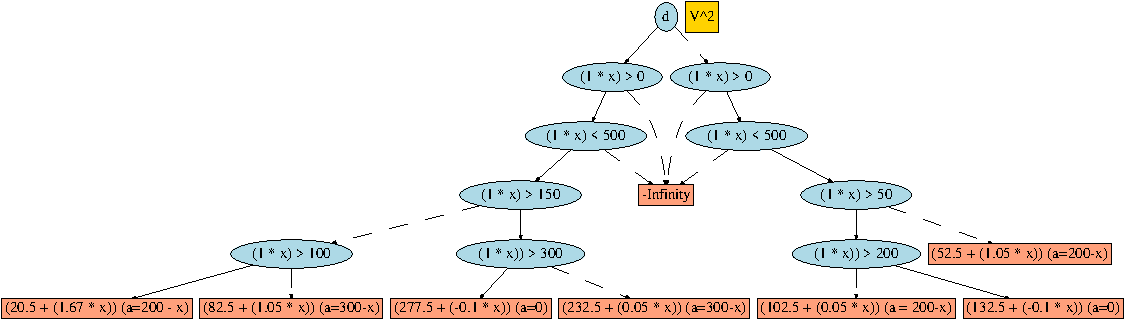
\includegraphics[width=1 \textwidth]{Figures2/diagrams/v2_inv2_2.pdf}
\begin{subfigure}
                \centering
                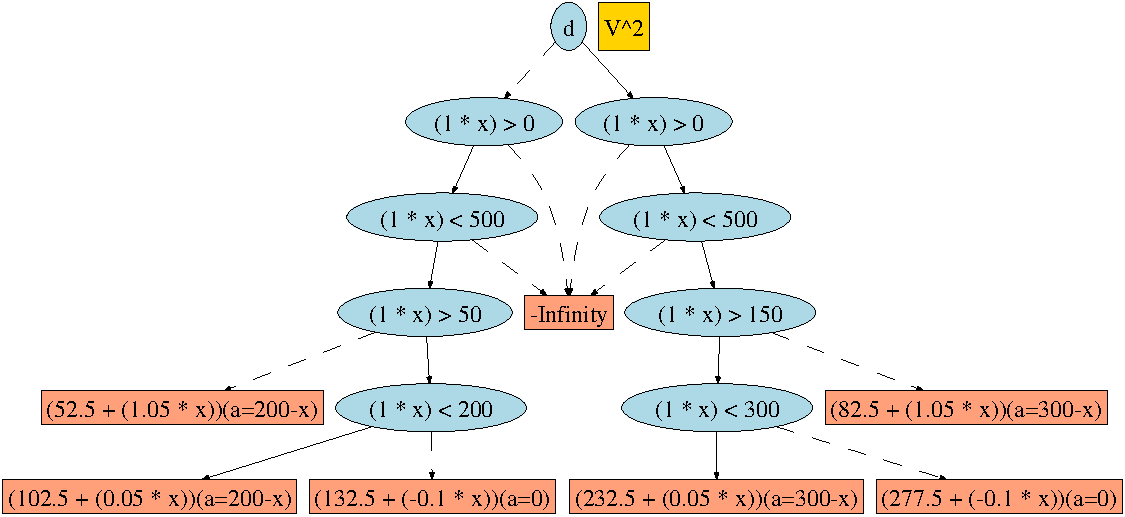
\includegraphics[width=0.68\textwidth]{pics/inv-v2.pdf}
        \end{subfigure}
                \hspace{2mm}
\begin{subfigure}
                \centering
                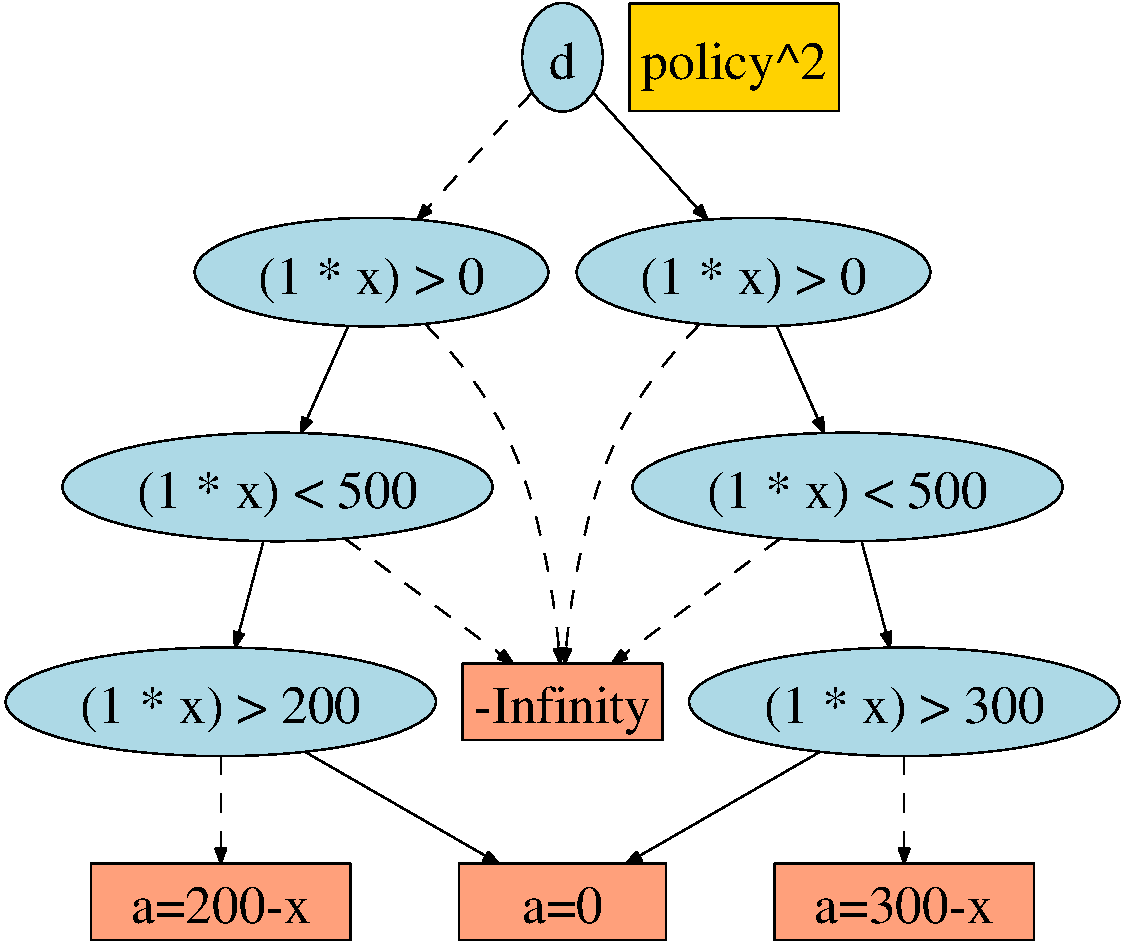
\includegraphics[width=0.26\textwidth]{pics/inv-p2.pdf}
        \end{subfigure}
\vspace{-2mm}
\caption{\footnotesize Optimal value function $V^2(x)$ for the
CAIC problem represented as an extended algebraic decision
diagram (XADD).  Here the solid lines represent the $\true$ branch for
the decision and the dashed lines the $\false$ branch.  To evaluate
$V^2(x)$ for any state $x$, one simply traverses the diagram in a
decision-tree like fashion until a leaf is reached where the
non-parenthetical expression provides the \emph{optimal value} and the
parenthetical expression provides the \emph{optimal policy} 
($a = \pi^{*,2}(x)$) to achieve value $V^2(x)$ (Left); Simplified diagram for the optimal policy for the second iteration $\pi^2$ consistent with Scarf's policy (Right).}
\label{fig:inv_policy}
\vspace{-6mm}
\end{figure}
%%%%%%%%%%%%%%%%%%%%%%%%%%%%%%%%%%%%%%%%%%%%%%%%%%%%%%%%%%%%%%%%%%%%%%%%%%
Note that illegal state values are defined using $-\infty$, in this case having the capacity lower than zero at any time and having capacity higher than that of the total $C$. 
\end{example*}

If our objective is to maximize the long-term \emph{value} $V$ (i.e. the sum of rewards received over an infinite horizon of actions), we show that the optimal value function can be derived in closed-form. 
For a single-item CAIC problem \footnote{For purposes of concise exposition and explanation
of the optimal value function and policy, this example uses
continuous univariate state and action;
the empirical results will later discuss a range of HMDPs with
multivariate hybrid state and action.}
the optimal value function for the second horizon is defined in Figure~\ref{fig:inv_policy} (left):
\vspace{-3mm}
\begin{align}
V = \begin{cases}
(x < 0 \vee x>500) &: -\infty \\
d \land (0 \leq x \leq 500) \land (x \geq 300) &:  277.5 - 0.1 * x \\
d \land (150 \leq x \leq 300) &:  232.5 + 0.05 * x \\
d \land ( 0 \leq x \leq 150) &:  82.5 + 1.05 * x \\
\neg d \land (200 \leq x \leq 500)  &:  132.5 - 0.1 * x \\
\neg d \land (50 \leq x \leq 200) &: 102.5 + 0.05 * x \\
\neg d \land (0 \leq x \leq 50) &:  52.5 + 1.05 * x \\
\end{cases} \label{eq:vfun_inv}
%\vspace{-7mm}
\end{align}
The policy obtained from this piecewise and linear value function and $V^2$ itself are shown in Figure~\ref{fig:inv_policy} using an extended algebraic decision diagram (XADD) representation which allows efficient implementation of the \emph{case calculus} for arbitrary functions. According to Scarf's policy for the \InventoryControl problem, if the holding and storage costs are linear the optimal policy in each horizon is always of $(S,s)$ ~\cite{Scarf_Karlin58}. In general this means if ($x>s$) the policy should be not to order any items and if ($x<s$) then ordering $S-s-x$ items is optimal. 
%%%%%%%%%%%%%%%%%%%%%%%%%%%%%%%%%%%%
According to this we can rewrite Scarf's policy where each slice of the state space matches with this general rule: 
\begin{align}
\pi^{*,2}(x) = 
\begin{cases}
(x < 0 \vee x>500) &: -\infty \\
d \land (300 \leq x \leq 500)  &:  0 \\
d \land (0 \leq x \leq 300) &:  300 - x \\
\neg d \land (200 \leq x \leq 500) &:  0 \\
\neg d \land (0 \leq x \leq 200) &:  200 - x \\
\end{cases}\nonumber
\end{align}

While this simple example illustrates the power of using continuous variables, for a multi-variate problem it is the very \textit{first solution} to exactly solving problems such as the DAIC and CAIC. 
We propose novel ideas to work around some of the expressiveness limitations of previous approaches, significantly generalizing the range of HMDPs that can be solved exactly.  To achieve this more general solution, this
paper contributes a number of important advances:
\begin{itemize}
\item The use of case calculus allows us to perform Symbolic dynamic programming (SDP) \cite{fomdp} used to solve MDPs with
piecewise transitions and reward functions defined in first-order logic. We define all required operations for SDP such as $\oplus,\ominus,max,min$ as well as new operations such as the continuous maximization of an action parameter $y$ defined as $max_y$ and integration of discrete noisy transition.
\item We perform value iteration for two different settings. In the first setting of DA-HMDP we consider continuous state variables with a discrete action set while in the second setting CA-HMDP we consider continuous states and actions. Both DA-HMDPs and CA-HMDPs are evaluated on various problem domains. The results show that DA-HMDPs applies to a wide range of transition and reward functions providing hyper-rectangular value functions. CA-HMDPs have more restriction in modeling due to the increased complexity caused by continuous actions, and limit solutions to linear and quadratic transitions and rewards but provide strong results for many problems never solved exactly before. 
\item While the \emph{case} representation for the optimal \textsc{CAIC} 
solution shown in \eqref{eq:vfun_inv} is sufficient in theory to
represent the optimal value functions that our HMDP solution
produces, this representation is unreasonable to maintain in practice
since the number of case partitions may grow exponentially on
each receding horizon control step.  For \emph{discrete} factored
MDPs, algebraic decision diagrams (ADDs) \cite{bahar93add} have been
successfully used in exact algorithms like SPUDD \cite{spudd} to
maintain compact value representations.  Motivated by this work we
introduce extended ADDs (XADDs) to compactly represent general
piecewise functions and show how to perform efficient operations on
them \emph{including} symbolic maximization.  Also we present all properties and algorithms required for XADDs. 
\end{itemize}

Aided by these algorithmic and data structure advances, we empirically demonstrate that our SDP approach with XADDs can exactly solve a variety of HMDPs with discrete and continuous actions. 


\section{Hybrid MDPs (HMDPs)}
The mathematical framework of Markov Decision Processes (MDPs) is used for modelling many stochastic sequential decision making problems ~\cite{bellman}. This discrete-time stochastic control process chooses an action $a$ available at state $s$. The process then transitions to the next state $s'$ according to $\mathcal{T}(s,s')$ and receives a reward $\mathcal{R}(s,a)$. The transition function follows the Markov property allowing each state to only depend on its previous state.  We provide novel exact solutions using the MDP framework for discrete and continuous variables in the state and action space. Hybrid state and action MDPs (HMDPs) are introduced in the next section followed by the finite-horizon solution via dynamic programming ~\cite{li05}.
%\vspace*{-0.05in}
\subsection{Factored Representation}
\label{sec:HMDPs}
%\vspace*{-0.05in}
The formal definition of a hybrid MDP (HMDP) is presented in the following: 
\begin{itemize}
\item States are represented by vectors of variables $(\vec{b},\vec{x}) = ( b_1,\ldots,b_n,x_{1},\ldots,x_m )$.  We assume
that each $b_i \in \{ 0,1 \}$ ($1 \leq i \leq m$) is boolean$\,$ and each $x_j \in \mathbb{R}$ ($1 \leq j \leq
n$) is continuous.

\item A finite set of $p$ actions $A = \{a_{1}(\vec{y}_1), \ldots, a_{p}(\vec{y}_p)\}$, where each action $a_k(\vec{y_k})$ ($1
\leq k \leq p$)  with parameter $\vec{y}_k \in \mathbb{R}^{|\vec{y}_k|}$  denotes continuous parameters for 
action $a_{k}$ and  if $|\vec{y}_k|=0$ then action $a_{k}$ has no parameters and is a discrete action.

\item The state transition model $\mathit{P}(\vec{b}',\vec{x}'|\vec{b},\vec{x},a,\vec{y})$, which specifies the
probability of the next state $(\vec{b}',\vec{x}')$ conditioned on a
subset of the previous and next state and action $a$ with its possible parameters $\vec{y}$; 

\item Reward function $\mathcal{R}(\vec{b},\vec{x},\vec{b}',\vec{x}',a,\vec{y})$, which specifies the immediate reward obtained by taking action $a(\vec{y})$ in state $(\vec{b},\vec{x})$; 

\item Discount factor $\gamma, \; 0 \leq \gamma \leq 1$.
\footnote{If time is explicitly included as one of the
continuous state variables, $\gamma = 1$ is typically used, unless
discounting by horizon (different from the state variable time) is
still intended.}  
\end{itemize}

A policy $\pi$ specifies the action $a(\vec{y}) =\pi(\vec{b},\vec{x})$ to take in each state $(\vec{b},\vec{x})$.  Our
goal is to find an optimal sequence of finite horizon-dependent
policies
%put footnote back in
\footnote{We assume a finite horizon $H$ in this
paper, however in cases where our SDP algorithm converges
in finite time, the resulting value function and 
corresponding policy are optimal for $H=\infty$. 
For finitely bounded value
with $\gamma = 1$, the forthcoming SDP algorithm may terminate in
finite time, but is not guaranteed to do so; for $\gamma < 1$, an
$\epsilon$-optimal policy for arbitrary $\epsilon$ can be computed by
SDP in finite time.
} 
$\Pi^* = (\pi^{*,1},\ldots,\pi^{*,H})$ that
maximizes the expected sum of discounted rewards over a horizon $h \in H; H \geq 0$:
\begin{align}
V^{\Pi^*}(\vec{x}) & = E_{\Pi^*} \left[ \sum_{h=0}^{H} \gamma^h \cdot r^h \Big| \vec{b}_0,\vec{x}_0 \right]. \label{eq:vfun_def}
\end{align}
Here $r^h$ is the reward obtained at horizon $h$ following $\Pi^*$ where 
we assume starting state $(\vec{b}_0,\vec{x}_0)$ at $h=0$.

 %%%%%%%%%%%%%%%%%%%%%%%%%%%%%%%%%%%%%%%%%%%%%%%%%%%%%%%%%%%%%%%%%%%%%%%%%%
%\vspace{10mm}
\begin{figure}[t!]
%\centering
%\subfigure{
%\hspace{-20mm}
%\vspace{-6mm}
 \begin{subfigure}
                \centering
                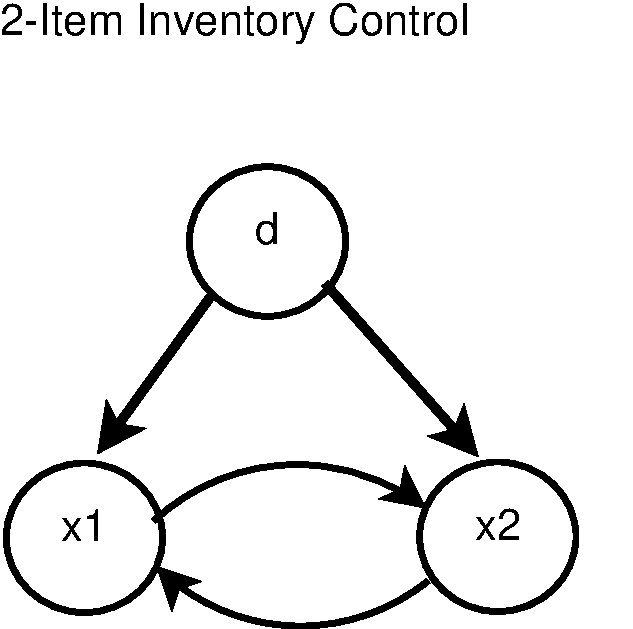
\includegraphics[width=0.2\textwidth]{pics/dbn_state.pdf}
        \end{subfigure}
                \hspace{2mm}
\begin{subfigure}
                \centering
                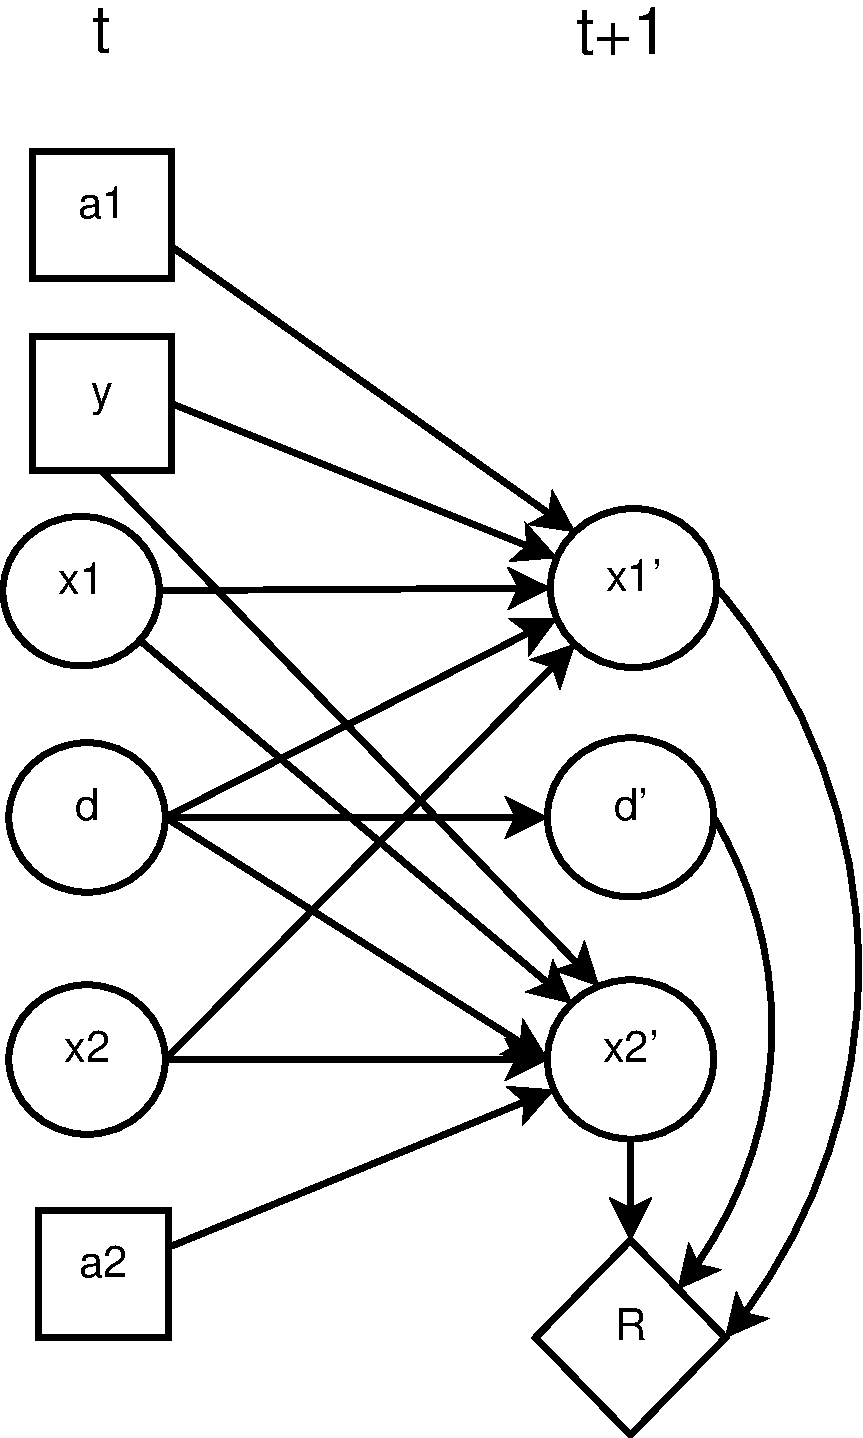
\includegraphics[width=0.22\textwidth]{pics/dbn_inv2.pdf}
        \end{subfigure}
                        \hspace{-1mm}
\begin{subfigure}
                \centering
                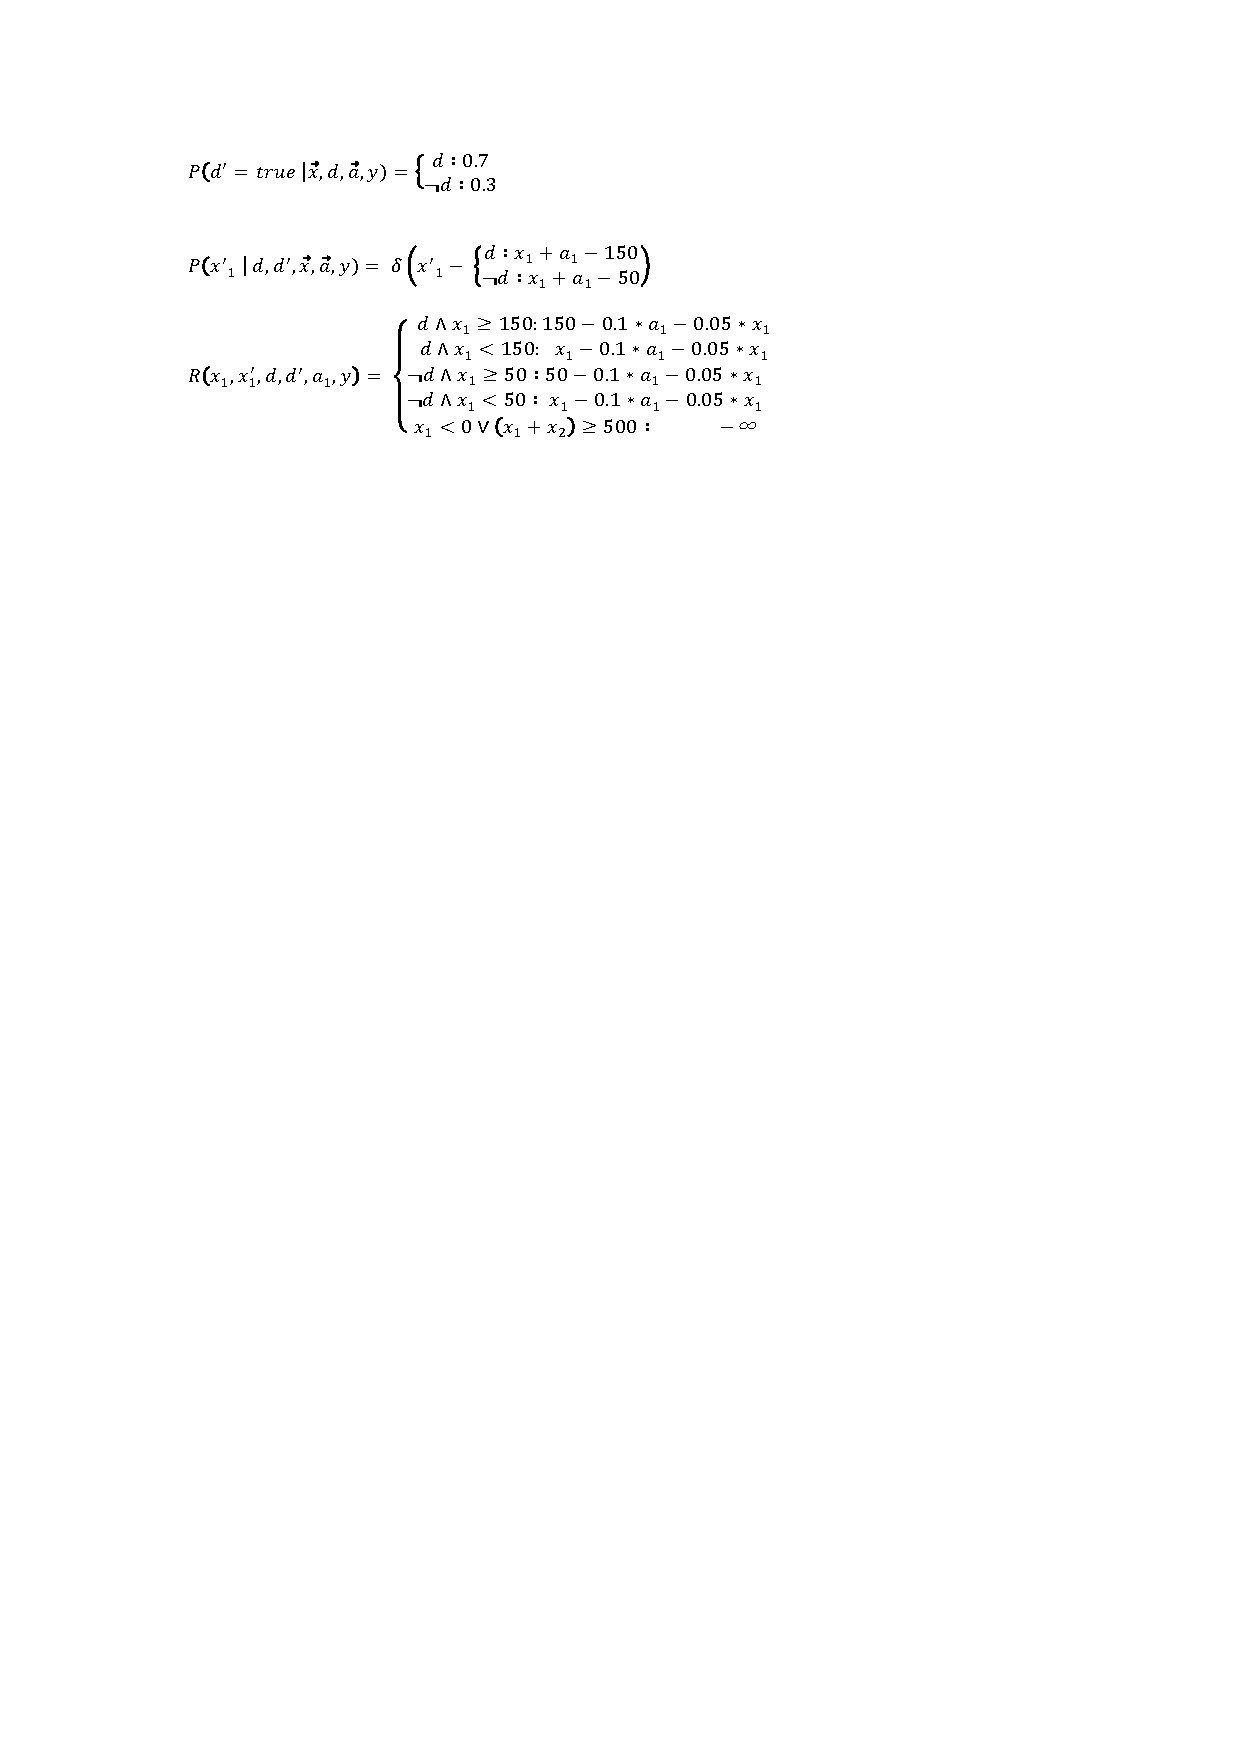
\includegraphics[width=0.52\textwidth]{pics/probabilities_2.pdf}
        \end{subfigure}
       % \vspace{-3mm}
\caption{%\footnotesize 
{\it (left)} Network topology between state variables in the 2-item continuous action \InventoryControl (CAIC) problem; {\it (middle)} DBN structure representing the transition and reward function; {\it (right)} transition probabilities and reward function in terms of CPF and PLE for $x_1$. }
\label{fig:dbn}
%\vspace{-3mm}
\end{figure}
%%%%%%%%%%%%%%%%%%%%%%%%%%%%%%%%%%%%%%%%%%%%%%%%%%%%%%%%%%%%%%%%%%%%%%%%%%

Such HMDPs are naturally factored \cite{boutilier99dt}
in terms of state variables $(\vec{b},\vec{x},\vec{y})$ where potentially $\vec{y} =0$. The transition structure can be exploited in the form of a dynamic Bayes
net (DBN) \cite{dbn} where the conditional probabilities
$P(b_i'|\cdots)$ and $P(x_j'|\cdots)$ for each next state variable can
condition on the action, current and next state. 
We can also have \emph{synchronic arcs} (variables that condition on each
other in the same time slice) within the binary $\vec{b}$ or
continuous variables $\vec{x}$ and from $\vec{b}$ to $\vec{x}$.%\footnote{Synchronic arcs between variables within $\vec{b}$ or within $\vec{x}$ can be accommodated if the forthcoming Algorithm~\ref{alg:regress} (\texttt{Regress}) is modified to multiply and marginalize-out multiple next-state variables in one elimination step according to the DBN structure.}  
Hence we can factorize the joint transition model as
{%\footnotesize
\begin{equation}
P(\vec{b}',\vec{x}'|\vec{b},\vec{x},a,\vec{y}) = 
\prod_{i=1}^n P(b_i'|\vec{b},\vec{x},\vec{b'},\vec{x'},a,\vec{y}) \prod_{j=1}^m P(x_j'|\vec{b},\vec{b}',\vec{x},\vec{x'},a,\vec{y}). \nonumber 
\end{equation}}
where $P(b_i'|\vec{b},\vec{x},\vec{b'},\vec{x'},a,\vec{y})$ may condition on a subset of
$\vec{b}$ and $\vec{x}$ in the current and next state and likewise 
$P(x_j'|\vec{b},\vec{b}',\vec{x},\vec{x'},a,\vec{y})$ may condition on a subset of
$\vec{b}$, $\vec{b}'$, $\vec{x}$ and $\vec{x'}$. Figure~\ref{fig:dbn} presents the DBN for a 2-item CAIC example according to this definition.  

We call the conditional probabilities
$P(b_i'|\vec{b},\vec{x},\vec{b'},\vec{x'},a,\vec{y})$ for \emph{binary} variables $b_i$
($1 \leq i \leq n$) conditional probability functions (CPFs) --- not
tabular enumerations --- because in general these functions can
condition on both discrete and continuous state as
in the right-hand side of~\eqref{eq:trans_inv}.  For the \emph{continuous} variables
$x_j$ ($1 \leq j \leq m$), we represent the CPFs
$P(x_j'|\vec{b},\vec{b'},\vec{x},\vec{x'},a,\vec{y})$ with \emph{piecewise
linear equations} (PLEs) satisfying the following properties: 
\begin{itemize}
\item PLEs can only condition on the action, current state, and previous state variables
\item PLEs are deterministic meaning that to be represented by probabilities they
must be encoded using Dirac $\delta[\cdot]$ functions (example forthcoming)
\item PLEs are piecewise linear, where the piecewise conditions may be arbitrary logical combinations of $\vec{b}$, $\vec{b}'$ 
and linear inequalities over $\vec{x}$ and $\vec{x'}$.  
\end{itemize}

The transition function example provided in the left-hand side of~\eqref{eq:trans_inv} can be expressed in PLE format such as the right figure in Figure~\ref{fig:dbn}:
\begin{align*}
P(x'_1 | d, d',\vec{x},\vec{a}, y) = \delta \Bigg( x'_1 -  \begin{cases}
d  : & x_i + a_i - 150 \\
\neg d : & x_i + a_i - 50    
\end{cases} \Bigg) 
\end{align*}
The use of the $\delta[\cdot]$ function ensures that the PLEs are conditional
probability functions that integrates to 1 over $x'_j$; In more intuitive
terms, one can see that this $\delta[\cdot]$ is a simple way to encode
the PLE transition $x' = \left\{ \ldots \right.$ in the form of 
$P(x_j'|\vec{b},\vec{b'},\vec{x},\vec{x'},a,\vec{y})$.

%qualify the extent of stochasticity and other restrictions
While it will be clear that our restrictions do not permit general stochastic transition noise (e.g., Gaussian noise as in LQG control), they do permit discrete noise in the sense that
$P(x_j'|\vec{b},\vec{b'},\vec{x},\vec{x'},a,\vec{y})$ may condition on
$\vec{b'}$, which are stochastically sampled according to their CPFs.
\footnote{Continuous stochastic noise for the transition function is an on going work which allows us to model stochasticity more generally}
We note that this representation effectively allows modeling of
continuous variable transitions as a mixture of $\delta$ functions,
which has been used frequently in previous exact continuous state MDP
solutions \cite{feng04,hao09}.
% should I put this????
Furthermore, we note that our
DA-HMDPs representation is more general than \cite{feng04,li05,hao09} in that
we do not restrict the equations to be linear, but rather
allow it to specify \emph{arbitrary} functions (e.g., nonlinear). 

The reward function in DA-HMDPs is defined as \emph{arbitrary} function of the current state for each action $a \in A$. 
While  empirical examples throughout the paper will demonstrate the full expressiveness of our symbolic dynamic programming approach, we note that there are computational advantages to be had when the reward and transition case conditions and functions can be restricted to linear polynomials.  

Due to the same restrictions, for CA-HMDPs the reward function $R(\vec{b},\vec{b'},\vec{x},\vec{x'}, a,\vec{y})$ is defined as either of the following:

(i) a general piecewise linear function (boolean or linear conditions and linear values) as in equation~\eqref{rew_inv}; or

(ii) a piecewise quadratic function of univariate state and a linear function of univariate action parameters:
\begin{align}
R(x,x',d,d', a) & = \begin{cases}
\neg d \land x \geq -2 \land x \leq 2 : & 4 - x^2 \\
d \lor x < -2 \lor x > 2 : & 0
\end{cases} \nonumber 
\end{align}
%The reward function in a DA-HMDPs can potentially be defined as an \emph{arbitrary} function but to ensure computationally efficient results we assume piecewise linear boundaries that can be checked for consistency using a linear constraint feasibility checker, which we will later see is crucial for efficiency.

These transition and reward constraints will ensure that all derived functions in the solution of HMDPs adhere to the reward 
constraints.

%\vspace*{-0.05in}
\subsection{Solution methods}
\label{sec:soln}
Now we provide a continuous state generalization of {\it value
iteration} \cite{bellman}, which is a dynamic programming algorithm
for constructing optimal policies.  It proceeds by constructing a
series of $h$-stage-to-go value functions $V^h(\vec{b},\vec{x})$.
Initializing $V^0(\vec{b},\vec{x}) = 0$ we define the quality
$Q_a^{h}(\vec{b},\vec{x},\vec{y})$ of taking action $a(\vec{y})$ in state
$(\vec{b},\vec{x})$ and acting so as to obtain
$V^{h-1}(\vec{b},\vec{x})$ thereafter as the following:

\vspace{-4mm}
{%\footnotesize
\begin{align}
Q_a^{h}(\vec{b},\vec{x},\vec{y}) & = 
 \sum_{\vec{b}'} \hspace{-1.0mm} \int \hspace{-1.0mm} \left( \prod_{i=1}^n P(b_i'|\vec{b},\vec{x},\vec{b'},\vec{x'},a,\vec{y}) \prod_{j=1}^m P(x_j'|\vec{b},\vec{b}',\vec{x},\vec{x'},a,\vec{y}) \right) \label{eq:qfun} \\ 
& \Bigg[ R(\vec{b},\vec{b'},\vec{x},\vec{x'}, a,\vec{y}) + \gamma \cdot V^{h-1}(\vec{b}',\vec{x}') d\vec{x}'  \hspace{-0.2mm} \Bigg] \nonumber
\end{align}}
Given $Q_a^h(\vec{b},\vec{x},\vec{y})$ for each $a \in A$ where $\vec{y}$ can also be empty , we can proceed
to define the $h$-stage-to-go value function as follows:
\begin{align}
V^{h}(\vec{b},\vec{x}) & = \max_{a \in A} \max_{\vec{y} \in \mathbb{R}^{|\vec{y}|}} \left\{ Q^{h}_a(\vec{b},\vec{x},\vec{y}) \right\} \label{eq:vfun}
\end{align}

For discrete actions, maximization over the continuous parameter $\vec{y}$ is omitted. The $max_{\vec{y}}$ operator defined in the next section is required to generalize solutions from DA-HMDPs to CA-HMDPs.
If the horizon $H$ is finite, then the optimal value function is
obtained by computing $V^H(\vec{b},\vec{x})$ and the optimal
horizon-dependent policy $\pi^{*,h}$ at each stage $h$ can be easily
determined via $\pi^{*,h}(\vec{b},\vec{x}) = \argmax_a
\argmax_{\vec{y}} Q^h_a(\vec{b},\vec{x},\vec{y})$.  If the horizon $H
= \infty$ and the optimal policy has finitely bounded value, then
value iteration can terminate at horizon $h$ if $V^{h} = V^{h-1}$;
then $V^\infty = V^h$ and $\pi^{*,\infty} = \pi^{*,h}$.

In DA-HMDPs, we can always compute the value function in tabular form;
however, how to compute this for HMDPs with reward and transition
function as previously defined is the objective of the symbolic
dynamic programming algorithm that we define in the next section.

\section{Symbolic Dynamic Programming} \label{SDP}
As it's name suggests, symbolic dynamic programming (SDP) \cite{fomdp}
is simply the process of performing dynamic programming (in this case
value iteration) via symbolic manipulation. Specifically SDP provides symbolic abstraction of all functions which allows building distinct logical partitions on the state space to represent the policy and value function. While SDP as defined
in \cite{fomdp} was previously only used with piecewise
constant functions, we now generalize the representation to work with
general piecewise functions for HMDPs in this article. Using the \emph{mathematical} definitions of the previous section, we  
show how to \emph{compute} equations~\eqref{eq:qfun} and \eqref{eq:vfun} 
symbolically.
%Should all this be taken out?
%We present the general SDP framework for value iteration in DA-HMDPs in Algorithm~\ref{alg:vi} (\texttt{VI}). Further we define  Algorithm~\ref{alg:contMax}(\texttt{Continuous Maximization}) to deal with the final maximization in (~\ref{eq:vfun}) for continuous actions.

Before we define our solution, however, we must formally define our
case representation and symbolic case operators.

\subsection{Case Representation and Operations}
\label{sec:caserep}
The symbolic case representation presented in this section, extends the SDP framework in \cite{fomdp}, which addresses piecewise constant functions, to general piecewise functions. This allows an expressive representation of functions in the following case form:
{%\footnotesize 
\begin{align*}
f = 
\begin{cases}
  \phi_1: & f_1 \\ 
 \vdots&\vdots\\ 
  \phi_k: & f_k \\ 
\end{cases}
\end{align*}
}
Here, $\phi_i$ is a logical formulae over the hybrid state $(\vec{b},\vec{x}), \vec{b} \in \mathbb{B}^m, \vec{x} \in \mathbb{R}^n$ and is defined by arbitrary logical combinations ($\land,\lor,\neg$) of 
(1) boolean variables in $\vec{b}$ and (2) 
inequality relations ($\geq,>,\leq,<$) over continuous variables $\vec{x}$. 
The following example is a simple function in this case form: 
\begin{align*}
f_1 = 
\begin{cases}
b \wedge (x_1+x_2 >5) : & x_1+3 \\ 
\neg b \wedge (x_1+x_2 \leq 5) : & x_1+x_2 \\ 
\end{cases} 
\end{align*}

Each $\phi_i$ is disjoint from the other $\phi_j$ ($j \neq i$). However the $\phi_i$ may not exhaustively cover the state space. Hence $f$ may only be a partial function and undefined for some variable assignments. 
In general $f_i$ can be defined as an arbitrary function. However due to the restrictions mentioned later, for CA-HMDPs, we assume $f_i$ to be either linear or quadratic on $\vec{x}$. Similarly we assume $\phi_i$ is defined over linear inequalities.

In the next section, the main case operations required to perform SDP are presented. Note that if $f$ is continuous then all SDP operations preserve this continuous property. 

\subsubsection*{Scalar multiplication and Negation}
Unary operations include the scalar multiplication $c\cdot f$ (for
a constant $c \in \mathbb{R}$) and negation $-f$ on case statements. These unary operations are applied to each case partition
$f_i$ ($1 \leq i \leq k$) as follows:
{%\footnotesize
\begin{center}
\begin{tabular}{r c c l}
&
%\hspace{5mm}
  $c \cdot f = \begin{cases}
    \phi_1  : & c \cdot f_1 \\ 
   \vdots&\vdots\\ 
    \phi_k : & c \cdot f_k \\ 
  \end{cases}$
 &
\hspace{10mm}
  $-f = \begin{cases}
    \phi_1 : & - f_1 \\ 
   \vdots&\vdots\\ 
    \phi_k : & - f_k \\ 
  \end{cases}$
\end{tabular}
\end{center}
}
\subsubsection*{Binary operations}
For the binary operations of cross-sum $\oplus$, cross-product $\otimes$ or cross-minus $\ominus$ on two case statements, the cross-product
of the logical partitions of each case statement  $\phi_i$ and $\psi_j$ is used to perform the
corresponding operation:

{%\footnotesize 
\begin{center}
\begin{tabular}{r c c c l}
&
\hspace{-6mm} 
  $\begin{cases}
    \phi_1: & f_1 \\ 
    \phi_2: & f_2 \\ 
  \end{cases}$
$\oplus$
&
\hspace{-4mm}
  $\begin{cases}
    \psi_1: & g_1 \\ 
    \psi_2: & g_2 \\ 
  \end{cases}$
&
\hspace{-2mm} 
$ = $
&
\hspace{-2mm}
  $\begin{cases}
  \phi_1 \wedge \psi_1: & f_1 + g_1 \\ 
  \phi_1 \wedge \psi_2: & f_1 + g_2 \\ 
  \phi_2 \wedge \psi_1: & f_2 + g_1 \\ 
  \phi_2 \wedge \psi_2: & f_2 + g_2 \\ 
  \end{cases}$
\end{tabular}
\vspace{4mm}
\hspace{-2mm}

\hspace{-2mm}
\begin{tabular}{r c c c l}
&
\hspace{-6mm} 
  $\begin{cases}
    \phi_1: & f_1 \\ 
    \phi_2: & f_2 \\ 
  \end{cases}$
$\otimes$
&
\hspace{-4mm}
  $\begin{cases}
    \psi_1: & g_1 \\ 
    \psi_2: & g_2 \\ 
  \end{cases}$
&
\hspace{-2mm} 
$ = $
&
\hspace{-2mm}
  $\begin{cases}
  \phi_1 \wedge \psi_1: & f_1 \cdot g_1 \\ 
  \phi_1 \wedge \psi_2: & f_1 \cdot g_2 \\ 
  \phi_2 \wedge \psi_1: & f_2 \cdot g_1 \\ 
  \phi_2 \wedge \psi_2: & f_2 \cdot g_2 \\ 
  \end{cases}$
\end{tabular}
\vspace{4mm}
\hspace{-2mm}

\hspace{-2mm}
\begin{tabular}{r c c c l}
&
\hspace{-6mm} 
  $\begin{cases}
    \phi_1: & f_1 \\ 
    \phi_2: & f_2 \\ 
  \end{cases}$
$\ominus$
&
\hspace{-4mm}
  $\begin{cases}
    \psi_1: & g_1 \\ 
    \psi_2: & g_2 \\ 
  \end{cases}$
&
\hspace{-2mm} 
$ = $
&
\hspace{-2mm}
  $\begin{cases}
  \phi_1 \wedge \psi_1: & f_1 - g_1 \\ 
  \phi_1 \wedge \psi_2: & f_1 - g_2 \\ 
  \phi_2 \wedge \psi_1: & f_2 - g_1 \\ 
  \phi_2 \wedge \psi_2: & f_2 - g_2 \\ 
  \end{cases}$
\end{tabular}
\vspace{4mm}
\hspace{-2mm}
\end{center}
}
Some partitions resulting from
these operators may be inconsistent, that is $\phi_i \wedge \psi_j \models \perp$. In this case such a partition is discarded since it is irrelevant to the function value.

As explained in Section~\ref{sec:caserep} for CA-HMDPs, the functions $f_i$ and $g_i$ are restricted to be linear or quadratic in the continuous parameters. While $\oplus$ and $\ominus$ preserve this property (i.e. remain closed-form), for $\otimes$ the result could exceed the second order polynomial if either $f_i$ or $g_i$ are quadratic. In such cases we may only assume the other function is piecewise constant. Conveniently as we show in the SDP algorithm presented next that the cross-product only occurs for the multiplication of piecewise constants in piecewise linear or quadratic functions. Therefore it is safe to claim that all the binary operations defined above are closed-form.


\subsubsection*{Symbolic maximization}
For SDP, we also need to perform maximization over actions for~\eqref{eq:vfun} which is fairly straightforward
to define:
%\vspace{-5mm}

{%\footnotesize
\begin{center}
\begin{tabular}{r c c c l}
&
\hspace{-9mm} $\casemax \Bigg(
  \begin{cases}
    \phi_1: & f_1 \\ 
    \phi_2: & f_2 \\ 
  \end{cases}$
$,$
&
\hspace{-4mm}
  $\begin{cases}
    \psi_1: & g_1 \\ 
    \psi_2: & g_2 \\ 
  \end{cases} \Bigg)$
&
\hspace{-4mm} 
$ = $
&
\hspace{-4mm}
  $\begin{cases}
  \phi_1 \wedge \psi_1 \wedge f_1 > g_1    : & f_1 \\ 
  \phi_1 \wedge \psi_1 \wedge f_1 \leq g_1 : & g_1 \\ 
  \phi_1 \wedge \psi_2 \wedge f_1 > g_2    : & f_1 \\ 
  \phi_1 \wedge \psi_2 \wedge f_1 \leq g_2 : & g_2 \\ 
  \phi_2 \wedge \psi_1 \wedge f_2 > g_1    : & f_2 \\ 
  \phi_2 \wedge \psi_1 \wedge f_2 \leq g_1 : & g_1 \\ 
  \phi_2 \wedge \psi_2 \wedge f_2 > g_2    : & f_2 \\ 
  \phi_2 \wedge \psi_2 \wedge f_2 \leq g_2 : & g_2 \\ 
  \end{cases}$\label{symbolicMax}
\end{tabular}
\end{center}
}

For CA-HMDPs, if all $f_i$ and $g_i$ are linear, the $\casemax$ result is clearly still linear. If the $f_i$ or $g_i$ are quadratic with univariate variables (i.e. no bilinear terms such as $x_1x_2$), the expressions $f_i > g_i$ or $f_i \leq
g_i$ will be at most univariate quadratic. Any such constraint
can then be \emph{linearized} into a combination of at most 
two linear inequalities (unless tautologous or inconsistent) 
by completing the square (e.g., 
%$x^2 + 8x > 0 \equiv [x + 4]^2 > 4 \equiv [x \leq -2] \lor [x > 6]$
$-x^2 + 20x - 96 > 0 \equiv [x - 10]^2 \leq 4 \equiv [x > 8] \land [x \leq 12]$).  Hence
the result of this $\casemax$
operator will be representable in the restricted case format assumed in this paper
(i.e. linear inequalities in decisions). 

The key observation here is the case statements are closed under the binary operation of continuous case maximization (or minimization). Additionally while it may seem that this operation leads to a blowup in the number of case partitions, the XADDs presented in the next section can exploit the internal structure of the continuous case maximization to represent it more compactly. 

Furthermore, the 
XADD that we introduce later will be able to exploit the 
internal decision structure of this
maximization to represent it much more compactly.

\subsubsection*{Restriction}
In restriction $f|_{\phi}$ %is fairly simple: in this operation, 
we want to restrict a function $f$ to apply only in cases
that satisfy some formula $\phi$.  
By appending $\phi$ to each case partition we make sure that all partitions must satisfy $\phi$:

{%\footnotesize
\begin{center}
\begin{tabular}{r c c l}
&
\hspace{-6mm} 
  $f = \begin{cases}
    \phi_1: & f_1 \\ 
   \vdots&\vdots\\ 
    \phi_k: & f_k \\ 
  \end{cases}$
&

&
\hspace{-2mm}
  $f|_{\phi} = \begin{cases}
    \phi_1 \land \phi : & f_1 \\ 
   \vdots&\vdots\\ 
    \phi_k \land \phi : & f_k \\ 
  \end{cases}$
\end{tabular}
\end{center}
}
Since $f|_{\phi}$ only applies when $\phi$ holds and is
undefined otherwise, $f|_{\phi}$ is partial unless $\phi \equiv \top$.

\subsubsection*{Substitution}
Symbolic substitution takes
a set $\sigma$ of variables and their substitutions and applies it to function $f$. 
Consider $\sigma = \{ x_1' / (x_1 \hspace{-.8mm} + \hspace{-.8mm} x_2), x_2' / x_1^2 \hspace{-.3mm} \exp(x_2) \}$
, the left-hand side of $/$ represents the substitution variable and the
right-hand side of $/$ represents the expression that should be substituted in its place.  
The substitution of a non-case function $f_i$ with $\sigma$ 
is $f_i\sigma$. If
$f_i = x_1' + x_2'$ then using the $\sigma$ defined above $f_i\sigma = x_1 + x_2 + x_1^2 \exp(x_2)$.  

Substitution into case partitions $\phi_j$ is performed 
by applying $\sigma$ to each inequality operand. Consider the following example with the $\sigma$ definition of above: 
\begin{align*}
f &= \begin{cases}
 x_1' \leq \exp(x_2'): & x_1' + x_2' \\ 
 x_1' \geq \exp(x_2'): & x_1'^2 - 3x_2' \\ 
\end{cases}
\\
f \sigma &= \begin{cases}
 x_1 + x_2 \leq \exp(x_1^2 \exp(x_2)): & x_1 + x_2 + x_1^2 \exp(x_2) \\ 
 x_1 + x_2 \geq \exp(x_1^2 \exp(x_2)): & (x_1 + x_2)^2 - 3x_1^2 \exp(x_2) \\ 
\end{cases}
\end{align*}

Note that if $f$ has mutually exclusive partitions $\phi_i$ ($1 \leq i \leq k$)
then $f\sigma$ must also have mutually exclusive partitions. 
This is followed from the logical consequence that 
if $\phi_1 \land \phi_2 \models \bot$
then $\phi_1\sigma \land \phi_2\sigma \models \bot$.
In general the substitution on case statements of function $f$ is 
defined below:
{%\footnotesize
\begin{center}
\begin{tabular}{r c c l}
\hspace{-2mm}
  $f\sigma = \begin{cases}
    \phi_1\sigma: & f_1\sigma \\ 
   \vdots&\vdots\\ 
    \phi_k\sigma: & f_k\sigma \\ 
  \end{cases}$
\end{tabular}
\end{center}
}

\subsubsection*{Continuous Integration of the $\delta$-function}
Continuous integration evaluates the integral marginalization $\int_{x_j= - \infty}^{\infty} f(x_j)\delta[x_j - h(\vec{z})]$ over the continuous variable $x_j$ in a function $f$  where $h(\vec{z})$ can be defined as a case statement and $\vec{z}$ does not contain $x_j$. . 
This integration triggers the substitution $\sigma = \{ x_j / h(\vec{z}) \}$ on $f$, that is
\begin{align}
\int_{x_j =-\infty}^{\infty} f(x_j)
\delta\left[ x_j - \begin{cases}
    \phi_1: & h_1 \\ 
   \vdots&\vdots\\ 
    \phi_k: & h_k \\ 
  \end{cases} \right] dx_j =% f(x_j) \{ x_j / h(\vec{z}) \}   = 
  \begin{cases}
    \phi_1: & f \{ x_j / h_1 \} \\ 
   \vdots&\vdots\\ 
    \phi_k: & f \{ x_j/ h_k \}  \\ 
  \end{cases}. \label{eq:gen_int}
\end{align}

As an example consider the example $\delta\left[ x_1' - (2x_1 + x_2) \right]$. Using the provided function definition, the continuous integration is defined according to the following: 
\begin{align*}
f (x_1',x_1,x_2)&= \begin{cases}
    x'_1 \geq 5 : & x'_1 + x_2 \\ 
    x'_1 < 5: & x_1 \\ 
  \end{cases} 
 \\
 \int_{x_1'} f(x_1',x_1,x_2)\delta\left[ x_1'- (2x_1+x_2) \right] dx_1'&= \begin{cases}
   2x_1 + x_2 - 5 \geq 0 : & 2x_1 + 2x_2 \\ 
    2x_1 + x_2 -5  < 0 : & x_1 \\
  \end{cases}
  \end{align*}
 
For a generic $\delta$ function with multiple case partitions, each of the $f$ partitions above are replaced into the multiple partitions of $\delta$. Such non-nested case statements are then reduced back down to a nested case
statement using a simple approach:

\begin{align*}
    \begin{cases}
      \phi_1: & 
        \begin{cases}
          \psi_1: & f_{11} \\ 
          \psi_2: & f_{12}  \\ 
        \end{cases} \\
      \phi_2: & 
        \begin{cases}
          \psi_1: & f_{21} \\ 
          \psi_2: & f_{22}  \\ 
        \end{cases} \\
    \end{cases} & \; = \;
        \begin{cases}
          \phi_1 \land \psi_1: & f_{11} \\ 
          \phi_1 \land \psi_2: & f_{12}  \\ 
          \phi_2 \land \psi_1: & f_{21} \\ 
          \phi_2 \land \psi_2: & f_{22}  \\ 
        \end{cases} 
\end{align*}

%As For SDP operations, this integration is defined as $\int_{x_j'} f(x_j')\mathit{P}(x_j'|\cdots) dx_j'$ where $P(x_j'|\cdots)$
%is in the form $\delta[x_j' - h(\vec{z})]$.
%\footnote{As we see in subsequent , probabilities must be encoded using Dirac $\delta[\cdot]$ functions to ensure that a conditional probability function integrates to 1 over $x_j'$}
 
\subsubsection*{Continuous Maximization}
\emph{Continuous Maximization} of a variable $y$ is defined as $g(\vec{b},\vec{x}) := \max_{\vec{y}}
\, f(\vec{b},\vec{x},\vec{y})$ where we crucially note that 
\emph{the} maximizing $\vec{y}$ is a function
$g(\vec{b},\vec{x})$, hence requiring \emph{symbolic} 
constrained optimization.
We can rewrite $f(\vec{b},\vec{x},y)$ via 
the following equalities:
\footnote{The second line ensures that all illegal values are mapped to $-\infty$}

\begin{align}
\max_y f(\vec{b},\vec{x},y) & = 
\max_y \casemax_i \, \begin{cases}
\phi_i(\vec{b},\vec{x},y) : f_i(\vec{b},\vec{x},y) \nonumber \\
\neg \phi_i(\vec{b},\vec{x},y) : -\infty
\end{cases} 
\end{align} 
\begin{align}
& = \casemax_i \, \fbox{$\max_y \begin{cases}
\phi_i(\vec{b},\vec{x},y) : f_i(\vec{b},\vec{x},y) \\
\neg \phi_i(\vec{b},\vec{x},y) : -\infty
\end{cases}$} \label{eq:casemax_max}
\end{align} 

The first equality is a consequence of the mutual disjointness of the partitions in $f$.  
Also because 
$\max_y$ and $\casemax_i$ are commutative and may be reordered,
we can compute $\max_y$ for \emph{each case partition
individually}.  
The case statement in the first equality is to ensure that all illegal values are mapped to $-\infty$. For computing the result of a given function $F_1$ with $-infty$, we have $\casemax(F_1, -\infty) = F_1$. Thus this case statement is reduced to $\phi_i(\vec{b},\vec{x},y) f_i(\vec{b},\vec{x},y)$ for computing the maximum. 

Having handled the $-\infty$ case partition, we complete this section by
showing how to symbolically compute a single partition 
$\max_y \phi_i(\vec{b},\vec{x},y): f_i(\vec{b},\vec{x},y)$ represented in the second equality of Equation~\ref{eq:casemax_max}.

In $\phi_i$, we observe that each conjoined constraint serves one of
three purposes: 
\begin{itemize}
\item \emph{upper bound ($\UB$) on $y$}: can be written as $y < \cdots$ or $y \leq \cdots$
\item \emph{lower bound ($\LB$) on $y$}: it can be written as $y >\cdots$ or $y \geq \cdots$
\footnote{For purposes of evaluating
a case function $f$ at an upper or lower bound,
it does not matter whether a bound is inclusive ($\leq$ or $\geq$)
or exclusive ($<$ or $>$) since $f$ is required to be continuous
and hence evaluating at the limit of the inclusive bound will
match the evaluation for the exclusive bound.}
\item \emph{independent of $y$ ($\IND$)}: the constraints do not contain $y$
and can be safely factored outside of the $\max_y$.
\end{itemize}

Since there are multiple symbolic upper and lower
bounds on $y$, in general we will need to apply the $\casemax$
($\casemin$) operator to determine the highest lower bound $\LB$
(lowest upper bound $\UB$).

We also know that $\max_y \phi_i(\vec{b},\vec{x},y)
f_i(\vec{b},\vec{x},y)$ for a continuous function $f_i$ must occur at the critical points of the function --- 
either the upper or lower bounds ($\UB$ and $\LB$) of $y$, 
or the $\Root$ (i.e., zero) of $\frac{\partial}{\partial y} f_i$ 
w.r.t.\ $y$.  Each of $\UB$, $\LB$, and $\Root$
is a symbolic function of $\vec{b}$ and $\vec{x}$. 

Given the \emph{potential} maximal points of $y = \UB$, $y = \LB$, and
$y = \Root$ of $\frac{\partial}{\partial y} f_i(\vec{b},\vec{x},y)$
w.r.t. constraints $\phi_i(\vec{b},\vec{x},y)$ --- which are all
symbolic functions --- we must symbolically evaluate which yields the
maximizing value $\Max$ for this case partition:
\vspace{2mm}
{%\footnotesize
\begin{align*}
\Max =  \sq \begin{cases}
\mbox{$\exists \Root$}  \sq: \sq & \sqm \casemax( f_i \{ y / \Root \}, f_i \{ y / \UB \}, f_i \{ y / \LB \})\\
\mbox{else}  \sq:  \sq & \sqm \casemax( f_i \{ y / \UB \}, f_i \{ y / \LB \})
\end{cases}
\end{align*}}
Here $\casemax(f,g,h) = \casemax(f,\casemax(g,h))$.  The 
substitution operator $\{ y / f \}$ replaces $y$ with case statement $f$, 
defined previously.

At this point, we have almost completed the computation
of the $\max_y \phi_i(\vec{b},\vec{x},y) f_i(\vec{b},\vec{x},y)$
except for one issue: the incorporation of the independent ($\IND$) constraints
(factored out previously) and additional constraints that arise from the
symbolic nature of the $\UB$, $\LB$, and $\Root$.  

Specifically for the latter, we need to ensure that indeed $\LB \leq \Root \leq \UB$
(or if no root exists, then $\LB \leq \UB$) by building a set
of constraints $\CONS$ that ensure these conditions hold; to do this,
it suffices to ensure that for each possible expression $e$ used to
construct $\LB$ that $e \leq \Root$ and similarly for the $Root$ and $\UB$.
Now we express the final result as a single case partition:
\begin{equation*}
\max_y \phi_i(\vec{b},\vec{x},y) f_i(\vec{b},\vec{x},y) \;\; = \;\;
\left\{ \CONS \land \IND: \Max \right.
\end{equation*}
Hence, to complete the maximization for an entire case statement $f$, we need only apply the above procedure to each case partition of $f$ and then perform a symbolic $\casemax$ on all of the results. We further clarify this operation in the next section using the \InventoryControl  example.  

\subsection{Symbolic Dynamic Programming (SDP)}

%%%%%%%%%%%%%%%%%%%%%%%%%%%%%%%%%%%%%%%%%%%%%%%%%%%%%%%%%%%%%%%%%%%%%%%%
\incmargin{.5em}
\linesnumbered
\begin{algorithm}[t!]
%\vspace{-.5mm}
\dontprintsemicolon
\SetKwFunction{regress}{Regress}
\Begin
{
   $V^0:=0, h:=0$\;
   \While{$h < H$}
   {
       $h:=h+1$\;
       \ForEach {$a(\vec{y}) \in A$}
       {
              $Q_a^{h}(\vec{y})\,:=\,$\regress{$V^{h-1},a,\vec{y}$}\;
			  \emph{//Continuous action parameter}\;
			  \If  {$ \mid \vec{y} \mid >0$}  
               {
               $Q_a^{h}(\vec{y}) := \max_{\vec{y}} \, Q_a^{h}(\vec{y})$ $\,$ \;
               $\pi^{*,h} := \argmax_{a} \, Q_a^{h}(\vec{y})$\;
               } 
               \Else 
               { $\pi^{*,h} := \argmax_{a} \, Q_a^{h}(\vec{y})$ \; }
        }
       $V^{h} := \casemax \, Q_a^{h}(\vec{y})$ $\,$ \;
       \If{$V^h = V^{h-1}$}
           {break $\,$ \emph{// Terminate if early convergence}\;}
   }
     \Return{$(V^h,\pi^{*,h})$} \;
}
\caption{\footnotesize \texttt{VI}(HMDP, $H$) $\longrightarrow$ $(V^h,\pi^{*,h})$ \label{alg:vi}}
%\vspace{-1mm}
\end{algorithm}
\decmargin{.5em}
%%%%%%%%%%%%%%%%%%%%%%%%%%%%%%%%%%%%%%%%%%%%%%%%%%%%%%%%%%%%%%%%%
In this section the symbolic value iteration algorithm (SVI) for HMDPs is presented.
Our objective is to take a DA-HMDP or CA-HMDP as defined in Section~\ref{sec:HMDPs}, apply value
iteration as defined in Section~\ref{sec:soln}, and produce
the final value optimal function $V^h$ at horizon $h$ in the form
of a case statement presented in Algorithm~\ref{alg:vi}. 
We use the \textsc{CAIC} example from the introduction to help clarify each step of this algorithm. 

For the base case of $h=0$ in line 2, we note that setting $V^0(\vec{b},\vec{x}) = 0$
(or to the reward case statement, if it is not action dependent)
%and $R(\vec{b},\vec{x})$ as described in Section~\ref{sec:HMDPs}
is trivially in the form of a case statement.

%%%%%%%%%%%%%%%%%%%%%%%%%%%%%%%%%%%%%%%%%%%%%%%%%%%%%%%%%%%%%%%%%
\incmargin{.5em}
\linesnumbered
\begin{algorithm}[t!]
\vspace{-.5mm}
\dontprintsemicolon
\SetKwFunction{remapWithPrimes}{Prime}
%\SetKwFunction{sumout}{sumout}


\Begin{
    $Q=$ \remapWithPrimes{$V$} $\,$ \emph{// All $v_i \to v_i'$ ($\equiv$ all $b_i \to b_i'$ and all $ x_i \to x_i'$)} \;
%    \emph{// Continuous regression marginal integration}\\
%    \For {all $x'_j$ in $Q$}{
%         $Q := \int Q \otimes P(x_j'|\vec{b},\vec{b}',\vec{x},a,\vec{y}) \, d_{x'_j}$\;
%    }
%    \emph{// Discrete regression marginal summation}\\
%    \For {all $b'_i$ in $Q$}{
%         $Q := \left[ Q \otimes P(b_i'|\vec{b},\vec{x},a,\vec{y}) \right]|_{b_i' = 1}$\\
%         \hspace{8mm} $\oplus \left[ Q \otimes P(b_i'|\vec{b},\vec{x},a,\vec{y}) \right]|_{b_i' = 0}$\;
%    }
%    \Return{$R(\vec{b},\vec{x},a,\vec{y}) \oplus (\gamma \otimes Q)$} \;
\If {$v'$ in $R$}
	 {$Q := R(\vec{b},\vec{b}',\vec{x},\vec{x}',a,\vec{y}) \oplus (\gamma \cdot Q)$} \;
    \ForEach { $v'$ in $Q$}  
    {
    	\If {$v'$ = $x'_j$}
    	{
    	\emph{//Continuous marginal integration}\\
         $Q := \int Q \otimes P(x_j'|\vec{b},\vec{b}',\vec{x},\vec{x}',a,\vec{y}) \, d_{x'_j}$\;
    	}
	    \If {$v'$=$b'_i$}
    	{
    	\emph{// Discrete marginal summation}\\
         $Q := \left[ Q \otimes P(b_i'|\vec{b},\vec{b}',\vec{x},\vec{x}',a,\vec{y}) \right]|_{b_i' = 1}$
         $\oplus \left[ Q \otimes P(b_i'|\vec{b},\vec{b},\vec{x},\vec{x}',a,\vec{y}) \right]|_{b_i' = 0}$\;
    	}
    }
    \If {$\neg$ ($v'$  in $R$)}
    {$Q := R(\vec{b},\vec{b}',\vec{x},\vec{x}',a,\vec{y}) \oplus (\gamma \cdot Q)$ }\;
    \Return{$Q$} \;
}
\caption{\footnotesize \texttt{Regress}($V,a,\vec{y}$) $\longrightarrow$ $Q$ \label{alg:regress}}
\vspace{-1mm}
\end{algorithm}
\decmargin{.5em}
%%%%%%%%%%%%%%%%%%%%%%%%%%%%%%%%%%%%%%%%%%%%%%%%%%%%%%%%%%%%%%%%%

For $h > 0$ and for each action in line 5 we perform lines 6--12, starting with a call to Algorithm~\ref{alg:regress}.  Note that we have omitted parameters $\vec{b}$ and
$\vec{x}$ from $V$ and $Q$ to avoid notational clutter.
Fortunately, given our previously defined
operations, the (\texttt{Regress}) algorithm is can be performed using the following steps: 
\begin{enumerate}
\item {\it Prime the Value Function}: $V^{h}$ will be
the ``next state'' in value iteration thus the substitution operation of 
$\sigma = \{ b_1 / b_1', \ldots, b_n / b_n', x_1 / x_1', \ldots, x_m / x_m' \}$ is used to obtain
$V'^{h} = V^{h}\sigma$ in line 2 of Algorithm~\ref{alg:regress}. Starting with the first iteration, for the \textsc{CAIC} example this step does not apply to $h-1=0$ since $V^0=0$.
%where $V'^{h}$ is over $(\vec{b}',\vec{x}')$.

\item {\it Add Reward Function}: If the reward function $R$ contains any primed state variable $b'$ or $x'$, lines 3--4 of Algorithm~\ref{alg:regress} is executed to add this reward function to the previous discounted Q-value. If $R$ had no primed variables, then it is added to the Q-value at the end of Algorithm~\ref{alg:regress} in lines 14--15. The reward function of \textsc{CAIC} contains primed $x'$ thus the Q-value is defined as below: 

{%\footnotesize
\begin{align}
Q = \begin{cases}
(x < 0 \vee x>500 \vee x'<0 \vee x'<500) &: -\infty \\
d \land (150 \leq x \leq 500) &:  150 - 0.1 * a - 0.05 * x \\
d \land (0 \leq x \leq 150) &:  0.95 * x - 0.1 * a \\
\neg d \land (50 \leq x \leq 500) &: 50 + -0.1 * a+ -0.05 * x \\
\neg d \land (0 \leq x \leq 50) &:  0.95 * x + -0.1 * a\\
\end{cases} \nonumber
\end{align}}
\item {\it Continuous Integration}: The integral
marginalization over continuous variables $\int_{\vec{x}'}$ is performed in lines 7--9. According to the integration definition of the previous section,  this operation is performed repeatedly in sequence \emph{for each}
$x_j'$ ($1 \leq j \leq m$) and for every action $a$: 
\begin{align*}
\int_{x_j'} \delta[x_j' - g(\vec{x})] V'^{h} dx_j' \; = \; V'^{h} \{x_j' / g(\vec{x}) \}  
\end{align*} 
Following the \textsc{CAIC} example, the continuous integration of $x$ results in the following: 

{\footnotesize
\begin{align}
Q = \begin{cases}
x < 0 \vee x>500 &: -\infty \\
d \land (x \geq 150) \land (150 \leq (x+a) \leq 650) &:  150 - 0.1 * a - 0.05 * x \\
d \land (x \geq 150) \land ((x+a \geq 650) \vee (x+a \leq 150)) &:  -\infty \\
d \land (x \leq 150) \land (150 \leq (x+a) \leq 650)&:  0.95 * x - 0.1 * a \\
d \land (x \leq 150) \land ((x+a \geq 650) \vee (x+a \leq 150)) &:  -\infty \\
\neg d \land (x \geq 50) \land (50 \leq (x+a) \leq 550)  &:  50 - 0.1 * a - 0.05 * x \\
\neg d \land (x \geq 50) \land ((x+a \geq 550) \vee (x+a \leq 50)) &:  -\infty \\
\neg d \land (x \leq 50) \land (50 \leq (x+a) \leq 550) &:  0.95 * x - 0.1 * a \\
\neg d \land (x \leq 50) \land ((x+a \geq 550) \vee (x+a \leq 50)) &:  -\infty \\
\end{cases} \label{recent_q}
\end{align}
}

\item {\it Discrete Marginalization}: Given the partial
regression $Q^{h+1}$ for each action $a$ we next evaluate the discrete 
marginalization $\sum_{\vec{b}'}$ in~\eqref{eq:qfun} which is shown in lines 10--12 of Algorithm~\ref{alg:regress}.
Each variable $b_i'$ ($1 \leq i \leq n$)  is summed out independently using the restriction operation:
\begin{align*}
Q_a^{h+1} := & \left[ Q_a^{h+1} \otimes \mathit{P}(b_i'|\vec{b},\vec{x},\vec{b'},\vec{x'},a,\vec{y}) \right]|_{b_i' = 1} 
 \oplus \left[ Q_a^{h+1} \otimes \mathit{P}(b_i'|\vec{b},\vec{x},\vec{b'},\vec{x'},a,\vec{y}) \right]|_{b_i' = 0}.
\end{align*}
Note that both $Q_a^{h+1}$ and $\mathit{P}(b_i'|\cdots)$ can be represented
as case statements.
In \textsc{CAIC} discrete marginalization of the boolean state variable $d$ is not performed since there is no primed version of this variable ($d'$) in the current Q-function of ~\eqref{recent_q}. 
%Added algorithm
\end{enumerate}

Given the Q-function from Algorithm~\ref{alg:regress}, next we take the maximum over the continuous parameter $y$ of action variable $a(\vec{y})$ in line 8--9 of Algorithm~\ref{alg:vi}. Note that if the action were discrete $\mid \vec{y} \mid=0$ , lines 8--10 are not performed.

We can
rewrite any multivariate $\max_{\vec{y}}$ as a sequence of univariate
$\max$ operations $\max_{y_1} \cdots \max_{y_{|\vec{y}|}}$; hence it
suffices to provide just the \emph{univariate} $\max_y$ solution:
\begin{align}
\max_{\vec{y}} =\max_{y_1} \cdots \max_{y_{|\vec{y}|}} \Rightarrow g(\vec{b},\vec{x}) := \max_{y} \, f(\vec{b},\vec{x},y). \nonumber
\end{align}
Algorithm \ref{alg:contMax} outlines a univariate maximization  
$\max_y \phi_i(\vec{b},\vec{x},y) f_i(\vec{b},\vec{x},y)$ according to the previous section. 
\footnote{From here out we assume that all case partition conditions $\phi_i$ of
$f$ consist of conjunctions of non-negated linear inequalities and
possibly negated boolean variables --- conditions easy to enforce
since negation inverts inequalities, e.g., $\neg [x < 2] \equiv [x \geq 2]$
and disjunctions can be split across multiple non-disjunctive, 
disjoint case partitions.} 
Each step of this algorithm is followed using one of the partitions of the Q-function in (~\ref{recent_q}) in this case the first partition with the constraints and function value defined below: 
\begin{align*}
\phi_i(x,d,a) &\equiv d \land (0 \leq x \leq 500) \land (x \geq 150) \land ((x+a) \leq 650) \land ((x+a) \geq 150) \\
f_i(x,d,a) &= 150 - 0.1 * a - 0.05 * x
\end{align*}


%Added algorithm
%%%%%%%%%%%%%%%%%%%%%%%%%%%%%%%%%%%%%%%%%%%%%%%%%%%%%%%%%%%%%%%%%%%%%%%%
\incmargin{.5em}
\linesnumbered
\begin{algorithm}[t!]
\vspace{-.5mm}
\SetKwFunction{solveForVar}{SolveForVar}
\dontprintsemicolon
\Begin{
	$LB $ =$- \infty$ , 
	$UB$= $+ \infty$, 
	$IND,CONS $=$\mathit{true}$ , 
	$\mathit{Case_{max}} \,=\, \emptyset$ \;
     \For {$\phi_i \in f$ (\emph{For all partitions of $f$})}  
     {
     	\For{ $c_i \in \phi_i$ (\emph{For all conditions $c$ of $\phi_i$})}
     	{     		
     		\If {$c_i \leq y $} {$LB \,:=\, casemax(LB, c_i )$ \emph{//Add  $c_i$ to  LB, take max of all LBs}\; }
     		\If {$c_i \geq y $}	{$UB \,:=\, casemin(UB,c_i )$ \emph{//Add $c_i$ to  UB, take min of all UBs} \;	}
     		\Else {$IND \,:=\, [IND,c_i ]$ \emph{//Add constraint $c_i$ to  independent constraint set}\;}
     	}    	
     }
	$\mathit{Root}$ :=$ \solveForVar(y, f_i)$ \;
     	
     	\If {($\mathit{Root} \neq \mathit{null}$)}
     	 {
     	 		$CONS = (\mathbb{I} \left[ LB \right] \leq \mathbb{I} \left[ \mathit{Root} \right] ) 
     	 		\wedge (\mathbb{I} \left[ \mathit{Root} \right] \leq \mathbb{I} \left[ UB \right] )$\;
     	 } 
     	 \Else
     	  {
     	 	$CONS \,:=\, (\mathbb{I} \left[ LB \right] \leq \mathbb{I} \left[ UB \right])$\;
     	 }
     	\emph{//Conditions and value of continuous max for this partition\; }   
     	$\mathit{Max} \,:=\,  IND \wedge CONS : \casemax (f_i\left \lbrace y/LB \right \rbrace, f_i \left \lbrace y/UB \right \rbrace 		,f_i \left \lbrace y/ \mathit{Root} \right \rbrace)$\;
     	\emph{//Take maximum of this partition and all other partitions\;}       
     	$\mathit{Case_{max}} \,:=\, max(\mathit{Case_{max}} ,\mathit{Max}) $  
        
     \Return{$\mathit{Case_{max}} $} \;
}
\caption{\footnotesize \texttt{Continuous Maximization}($y$, $f(\vec{b},\vec{x},y)$) $\longrightarrow(max_{y}f(\vec{b},\vec{x},y))$ \label{alg:contMax}}
\vspace{-1mm}
\end{algorithm}
\decmargin{.5em}
%%%%%%%%%%%%%%%%%%%%%%%%%%%%%%%%%%%%%%%%%%%%%%%%%%%%%%%%%%%%%%%%%
To begin the set of lower bound $\LB$ is set to $-\infty$ and upper bound $\UB$ to $\infty$ so that any value larger than $-\infty$ is defined as the lower bound and any value lower than $+\infty$ is defined for $\UB$. Constraint variables $IND$ and $CONS$ are assumed to be true and the result of the $\casemax$ is set to empty. 

Each constraint $c_i$ in each partition $\phi_i$ is added to one of the sets of lower bound, upper bound or independent constraint as determined in lines 5--10. In our example this is equal to $\LB = (150 - x, 0) , \UB= (650 - x, 1000000) $ and $\IND=(d,x \geq 0 , x \leq 500) $ where the $0$ and $1000000$ are the natural lower and upper bounds on any inventory item $x$.
A unique $\LB$ and $\UB$ is defined by taking the maximum of the lower bounds and the minimum of the upper bounds as the best bounds in the current partition and the function \emph{SolveForVar} of line 13 takes any roots of the partition function (not applicable in the current partition): 
{%\footnotesize
\begin{align*}
\LB = \casemax(0,150-x) & = \begin{cases}
x > 150: & 0\\ 
x \leq 150: & 150 -x \\ 
\end{cases}\\
\UB = \casemin(100000, 650-x) & = \begin{cases}
x > -1000000: & 650 -x  \\ 
x \leq -1000000: &1000000\\ 
\end{cases}
\end{align*}
}  
The boundary constraints in lines 14--17 are added to the independent constraints as the constraint of the final maximum $\mathit{Max}$:
{\footnotesize 
\begin{equation*}
\CONS_{\LB \leq \UB} \sq = \sq [0 \leq 1000000] %\land [0 \leq 150 - x] 
\land [150 - x \leq 1000000] \land [150-x \leq 650 -x] \land [0 \leq 650 - x] 
\end{equation*}}
Here, two constraints are tautologies and may be removed.
A $\casemax$ is performed on the substituted $\LB$,$\UB$ and the roots on the function $f_i$: 
{\footnotesize 
\begin{align*}
 \Max &= \casemax \Big( f_i \{ y / \Root \} = \textit{null} , \\
 f_i \{ y / \LB \} &= \begin{cases}
x > 150: & \sqm 150 - 0.1 * (0) - 0.05 * x = 150 - 0.05 * x \\ 
x \leq 150:    & \sqm 150 - 0.1 * (150 - x ) - 0.05 * x = 135.00075 + 0.05 * x\\ 
\end{cases},\\
 f_i \{ y / \UB \} &= \begin{cases}
x > -1000000:    & \sqm 150 - 0.1 * (650 -x) - 0.05 * x = 84.980494 + 0.05 * x \\ 
x \leq -1000000: & \sqm 150 - 0.1 * (1000000) - 0.05 * x =  -99850 -0.05 * x\\ 
\end{cases} \Big) 
\end{align*}}
$\max_y$ is performed in line 19 for each partition using both independent and boundary constraints. The resulting maximum is according to the $\casemax$ operator defined in the previous section. Note that the partition of $x \leq -1000000:  -99850 -0.05 * x$ is omitted due to inconsistency.
{%\footnotesize 
\begin{align*}
\Max = 
\begin{cases}
(x > 150) \land (x \leq 650):    & \sqm 150 - 0.05 * x \\ 
(x > 150) \land (x \geq 650):    & \sqm 84.980494 + 0.05 * x \\ 
x \leq 150: & \sqm 135.00075 + 0.05 * x\\ 
\end{cases}
\end{align*}}
Returning to~\eqref{eq:casemax_max}, we have now specified the inner operation (shown in the $\Box$) for this partition after removing all redundant and inconsistent cases.\footnote{ These last two results are defined by taking out all inconsistent partitions. This is done using efficient pruning techniques mentioned in the previous section.}
\begin{align*}
\Max & = 
\begin{cases}
d \land (150 \leq x \leq 500):    & \sqm 150 - 0.05 * x \\ 
\text{\normalsize otherwise} : & -\infty\\ 
\end{cases}
\end{align*}
To complete the maximization for an entire case statement $f$, we need only apply the above procedure to each case partition of $f$ and then $\casemax$ all of these results in line 21: 
\begin{align*}
Q & = 
\begin{cases}
d \land (150 \leq x \leq 500):    & \sqm 150 - 0.05 * x \\ 
d \land (0 \leq x \leq 150):    & \sqm -14.99925 + 1.05 * x \\ 
\neg d \land (50 \leq x \leq 500):    & \sqm 50 - 0.05 * x \\ 
\neg d \land (0 \leq x \leq 50):    & \sqm -5 + 1.05 * x \\ 
\text{\normalsize otherwise} : & -\infty\\ 
\end{cases}
\end{align*}
To obtain the policy in Figure~\ref{fig:inv_policy}, 
we can annotate leaf values with any 
$\UB$, $\LB$, and $\Root$ substitutions performing line 10 or 12 in Algorithm~\ref{alg:vi}.

As the last step of Algorithm~\ref{alg:vi}, a case maximization is performed on the current Q-function. Given $Q_a^{h+1}(\vec{y})$ in
case format for each action $a \in\{a_{1}(\vec{y}_1), \ldots , a_{p}(\vec{y}_p)\}$, obtaining
$V^{h+1}$ in case format as defined in~\eqref{eq:vfun} requires
sequentially applying
\emph{symbolic maximization} in line 14:
\begin{align*}
V^{h+1} & = 
\max(Q_{a_1}^{h+1}(\vec{y}),\max(\ldots,\max(Q_{a_{p-1}}(\vec{y})^{h+1},Q_{a_p}^{h+1}(\vec{y}))))
\end{align*}
Note that for our \textsc{CAIC} example the last Q-function is equal to the optimal value function since we have considered a single continuous action here. %Line 10 and 12 in Algorithm~\ref{alg:vi} computes the optimal policy on the Q-function for the two action cases and line 14 performs symbolic maximization.
By induction, because $V^0$ is a case statement and applying
SDP to $V^h$ in case statement form produces $V^{h+1}$ in case
statement form, we have achieved our intended
objective with SDP. 

On the issue of correctness,
we note that each operation above simply implements one of the
dynamic programming operations in \eqref{eq:qfun} or \eqref{eq:vfun}, 
so correctness simply follows from verifying (a) that each case
operation produces the correct result and that (b) each case operation
is applied in the correct sequence as defined in \eqref{eq:qfun} or 
\eqref{eq:vfun}.  
Of course, that is the theory, next we meet practice.

\section{Extended Algebric Decision Diagrams (XADDs)} \label{XADD}

In the previous section all operations required to perform SDP algorithms were covered. The case statements represent arbitrary piecewise functions allowing general solutions to continuous problems. 
However as the previous section demonstrated, the final result of applying most operations such as binary operators and maximization is a larger case statement than the initial operands. Thus in practice it can be prohibitively expensive to maintain a tractable case representation. Maintaining a compact and efficient data structure for case statements is the key to SDP solutions.

Motivated by the SPUDD~\cite{spudd} algorithm which
maintains compact value function representations for finite discrete
factored MDPs using algebraic decision diagrams (ADDs)~\cite{bahar93add},
we extend this formalism to handle continuous variables in a data
structure we refer to as the XADD. 

Here we formally introduce this compact data structure of XADDs which can implement case statements efficiently along with pruning algorithms required to perform SDP operations.
 
 Figure~\ref{fig:inv_policy} of the introduction section demonstrates the value function for the \InventoryControl problem as an XADD representation. While XADDs are extended from ADDs, ADDs are extended from Binary decision diagrams (BDDs), allowing first-order logic instead of boolean logic. Figure~\ref{fig:bdd_add_xadd} demonstrates examples of the three decision diagrams of BDD, ADD and XADD as a comparison to show their expressiveness.   

A \emph{binary decision diagram} (BDD, \cite{bryant}) can represent propositional formulas or boolean functions ($\lbrace 0,1\rbrace^n \rightarrow \lbrace 0,1\rbrace$) as an ordered DAG where each node represents a variable and edges represent boolean assignment to  variables. Each decision node is a boolean test variable with two branches of low and high. The edge from the decision node to its low (high) successor represents assigning 0 (1) to its respective boolean variable. To evaluate the boolean function of a certain BDD under an assignment to its variables, the BDD is traversed by starting from the root node and following one of the low or high branches at each decision node until it reaches a leaf. The boolean value at the leaf is the value returned by this function according to the given variable assignment. 

%%%%%%%%%%%%%%%%%%%%%%%%%%%%%%%%%%%%%%%%%%%%%%%%%%%%%%%%%%%%%%%%%%%%%%%%%%
\begin{figure}[t!]
\centering
%\subfigure{
%\hspace{-20mm}
%\vspace{-3mm}
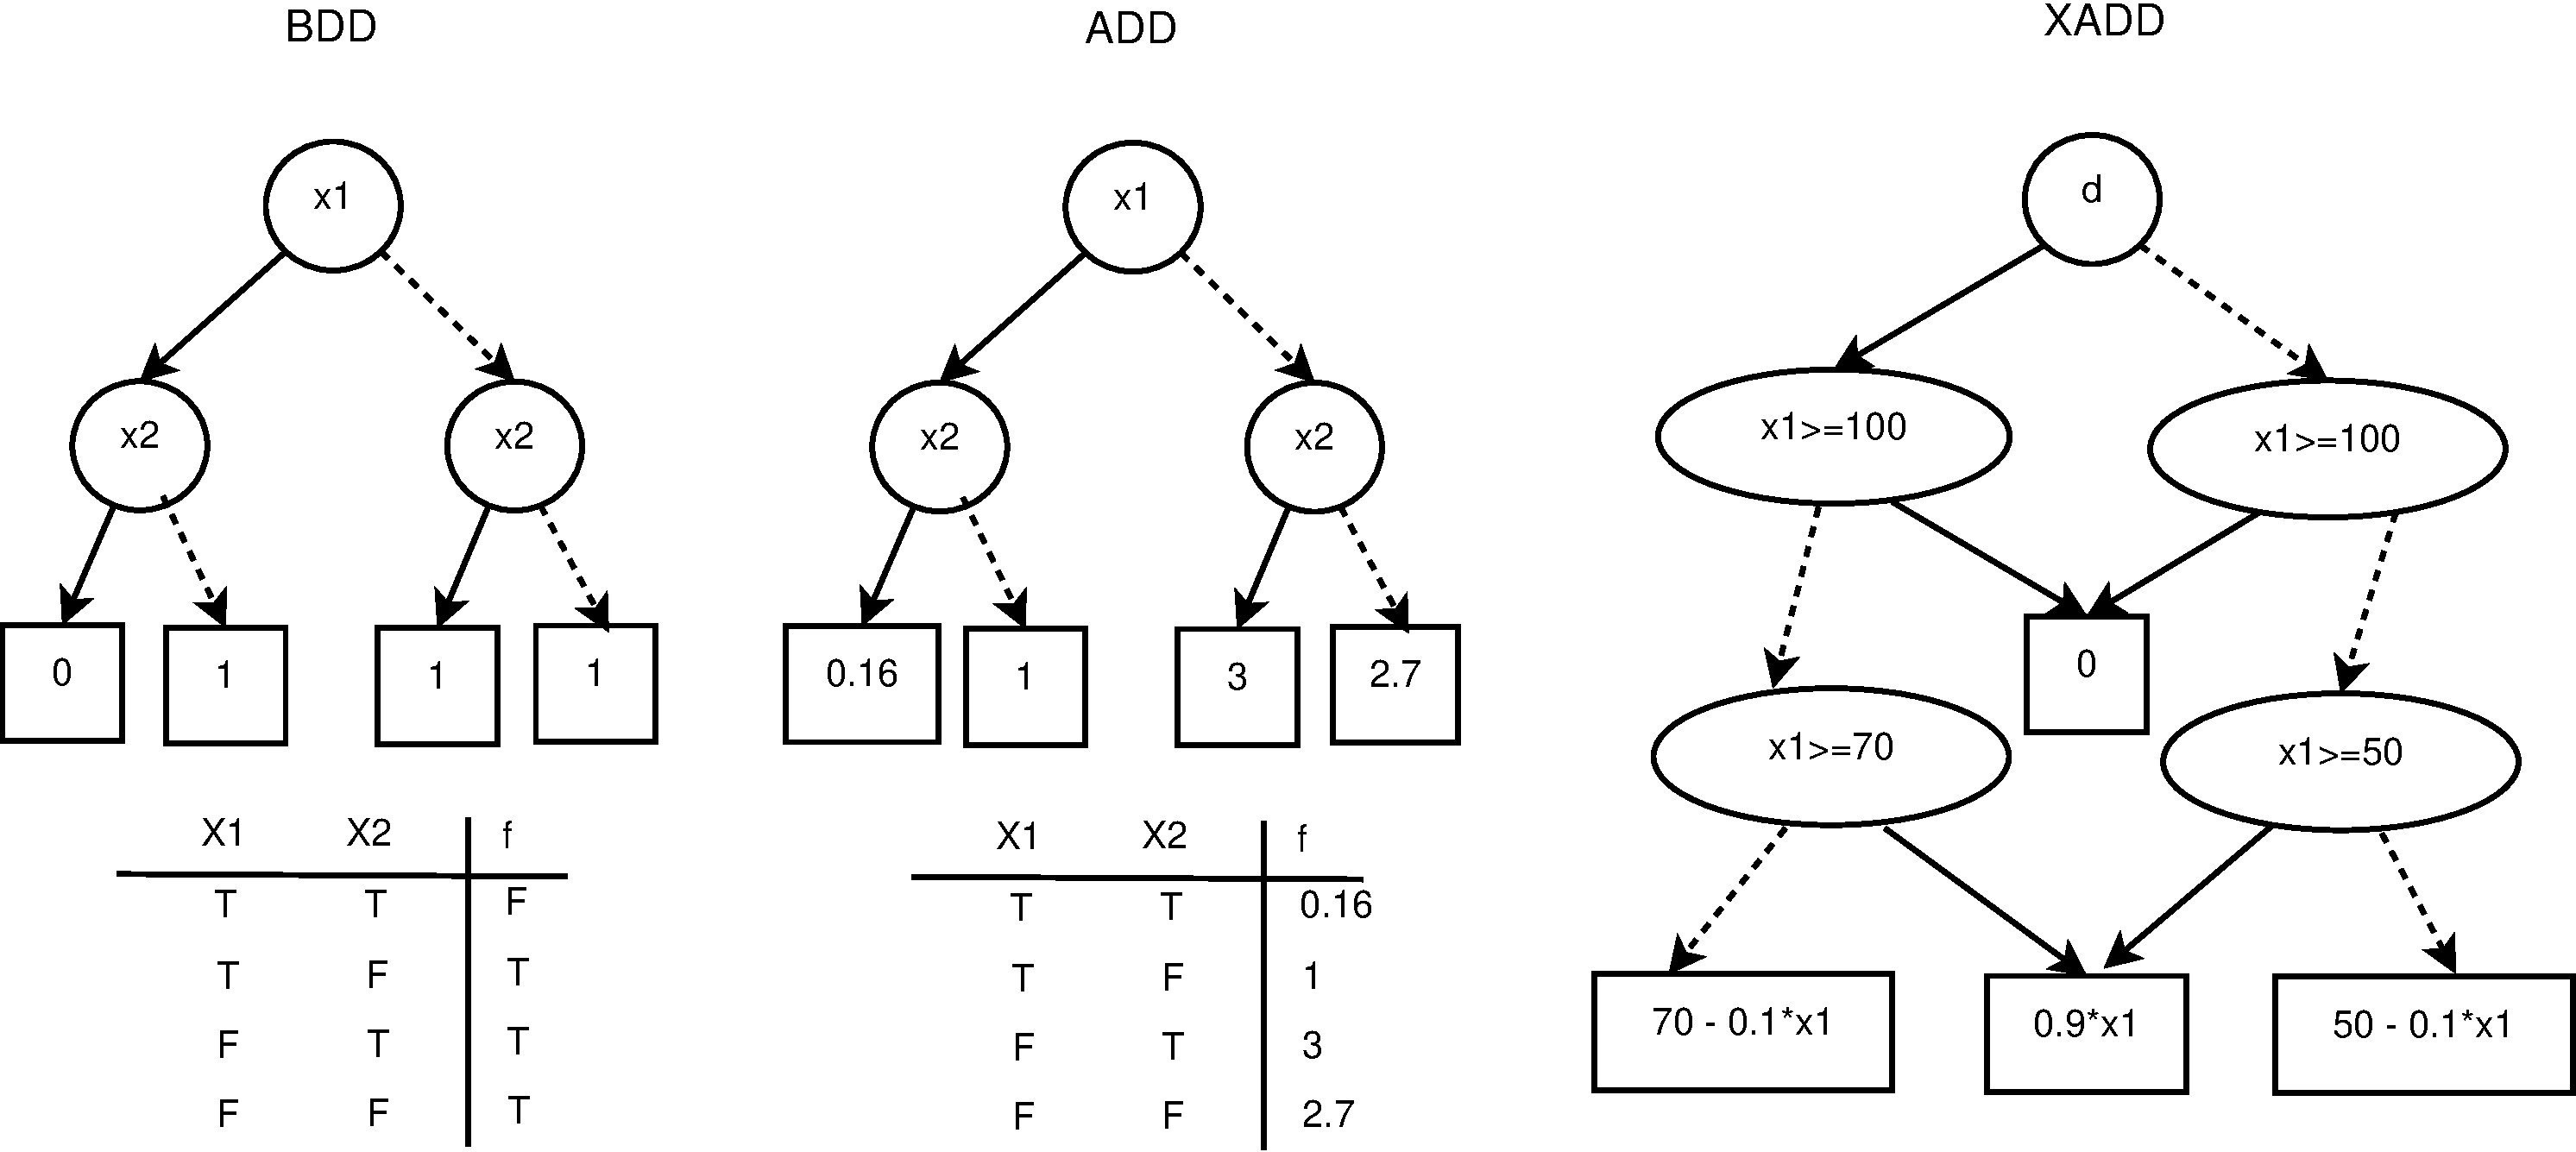
\includegraphics[width=0.8\textwidth]{pics/bdd_add_xadd.pdf}
\vspace{-1mm}

\caption{%\footnotesize
Comparison of three decision diagrams: {\it (left)} BDDs with boolean leaves and decisions representing $f(x_1,x_2) = x_1\bar{x_2}+\bar{x_1}$ as shown in the truth table; {\it (middle)} ADDs with  boolean decision nodes and real values at the leaves; {\it (right)} XADDs with polynomial leaves and decision nodes.}
\label{fig:bdd_add_xadd}
\end{figure}
%%%%%%%%%%%%%%%%%%%%%%%%%%%%%%%%%%%%%%%%%%%%%%%%%%%%%%%%%%%%%%%%%%%%%%%%%%

ADDs extend BDDs to allow real-valued ranges in the function representation ($\lbrace 0,1\rbrace^n \rightarrow \mathbb{R}$); they only differ from BDDs in the real-valued leaf nodes. There is a set of efficient operations for ADDs such as addition
($\oplus$), subtraction ($\ominus$), multiplication ($\otimes$),
division ($\oslash$), $\min(\cdot,\cdot)$ and $\max(\cdot,\cdot)$ (\cite{bahar93add}). Furthermore, BDDs and ADDs provide an efficient representation of CSI defined as the following: 
\begin{mydef}
The set of variables $A$ and $B$ are \emph{context-specifically independent} given the set of variables $C$ and the context $c \in C$, denoted by $A \perp B | (C=c)$, if the following holds: 
\begin{align}
\mathit{P}(A | B,C,c) = \mathit{P}(A|C,c) \hspace{2mm} whenever \hspace{2mm} \mathit{P}(B,C,c) >0. \label{def:csi}
\end{align}
\end{mydef}

%As a simple example of the CSI property, consider the ADD representation of Figure~\ref{fig:bdd_add_xadd} (middle). This ADD represents the transition probability of $\mathit{P}(X'_1| X_2, a_{move})$ where the probability of $X'_1$ only depends on $X_2, a_{move}$. However in the context of $a_{move} = \mathit{false}$, $X'_1$ is also independent from $X_2$ since the probability is always zero in this case, i.e. $\mathit{P}(X'_1| X_2, a_{move}) = \mathit{P}(X'_1|  a_{move} = \mathit{false})$. 

Parameterized ADD (PADD) is an extension of ADD that allows a compact representation of functions $\{0,1\}^{n} \rightarrow
\mathbb{E}$, where $\mathbb{E}$ is the space of expressions
parameterized by $\vec{p}$. For example, the ADD of Figure~\ref{fig:bdd_add_xadd} (middle) can be extended to a PADD to allow leaves such as $0.16p_1$ or $2.7+p_1$. PADDs are used as an efficient representation of factored MDPs with imprecise transitions (\cite{spuddip}). 

XADDs extend ADDs to allow representing functions with both boolean and continuous variables, i.e. $\{0,1\}^{m} \times \mathbb{R}^n \rightarrow \mathbb{R}$. Here decisions can be boolean variable tests or continuous inequalities and leaves can be defined as arbitrary continuous expressions. Similar to its predecessors XADDs are evaluated from root to leaf. 
We next formally define such XADDs with operations and algorithms required to support all case operations of SDP. Pruning algorithms are then introduced to make this representation even more efficient. We note that the formal definitions of our XADD are similar to that of PADD.

\subsection{Formal Definition and Operations}
An XADD is a function represented by a DAG on $\mathbb{R}$ with the domain $(\vec{b},\vec{x})$ where $b_i \in \{ 0,1 \}$ ($1 \leq i \leq m$) is boolean$\,$
and $x_j \in \left[ x_j^{min}, x_j^{max}\right]$ is continuous with $1 \leq j \leq n; x_j^{min}, x_j^{max} \in \mathbb{R}; x_j^{min}< x_j^{max}$.
According to Section~\ref{sec:caserep}, all functions can be represented using the case notation, therefore a case statement can be used to represent an XADD:
{%\footnotesize 
\begin{align}
f = 
\begin{cases}
  \phi_1(\vec{b},\vec{x}): & f_1 (\vec{x})\\ 
 \vdots&\vdots\\ 
  \phi_k(\vec{b},\vec{x}): & f_k(\vec{x}) \\ 
\end{cases} \label{eq:function_xadd}
\end{align}
}
here the $f_i$ are arbitrary expressions over $\vec{x}$ and $\phi_i(\vec{b},\vec{x})$ are logical formulae over $(\vec{b},\vec{x})$ and defined by arbitrary logical combinations ($\land,\lor,\neg$) of (a) boolean variables in $\vec{b}$ and (b) 
inequality relations ($\geq,>,\leq,<$) over continuous variables $\vec{x}$. 

In an XADD structure, each $f_i$ represents a leaf node and the $\phi_i(\vec{b},\vec{x})$ represent all decision node constraints leading to the leaf $f_i$. Also similar to decision trees, the DAG representation has a fixed ordering of decision tests from the root to a leaf where the low (l) or high (h) branch of each decision node determines the next node in the XADD. 

Similar to case statements that allow arbitrary functions, the above formulation represents a general XADD with arbitrary decision nodes and leaf expressions. However in this paper, we restrict our functions to linear decisions and linear leaf expressions. This allows us to prune inconsistent linear constraints using an LP-solver, resulting in a more compact XADD. Next we provide the mathematical definition of such \emph{linear XADDs} in the following: % Note that in the (or quadratic decisions that can be linearized). Also leaf expressions are assumed to be linear. 

\begin{mydef}(\textbf{Linear Leaf}):
A linear XADD leaf can be canonically defined using the set of continuous variables $\vec{x}$ and the set of constants $c_i$ as the following:
\begin{equation}
\mathit{linearLeaf} := c_0+\sum_{i} c_i x_i , 1 \leq i \leq n. 
\nonumber
\end{equation}
\end{mydef}

\begin{mydef}(\textbf{Linear XADD}):
Formally an XADD with linear decision and linear leaves is defined using the following BNF grammer: 
\begin{equation}
\nonumber
\begin{array}{lll}
F&::=&  \mathit{linearLeaf}  \hspace{1mm} \vert  \hspace{1mm} \mathrm{if} (\mathit{dec})\ \mathrm{then}\ F_h\ \mathrm{else}\ F_l \\
\mathit{dec} &::=& ( \mathit{linearLeaf} \leq 0)  \hspace{1mm}\vert \hspace{1mm}
 ( \mathit{linearLeaf} \geq 0) \vert \hspace{1mm} b\\
\mathit{linearLeaf} &::=&c_0+\sum_{i} c_i x_i\\
b&::=& 0|1.
\end{array}
\end{equation}
An XADD node $F$ is either a leaf node $\mathit{linearLeaf}$ with a linear expression value or a decision node $\mathit{dec}$ with two branches $F_h$ and $F_l$; both of the non-terminal type $F$. 

The decision node $\mathit{dec}$ can be a boolean decision test $b\in \lbrace 0,1 \rbrace$ or a linear inequality over continuous variables $\vec{x}$. Figure~\ref{fig:bdd_add_xadd} (right) represents an XADD consisting of leaf nodes such as node $0.9x$ or decision nodes such as nodes $b$ and $x \geq 100$. For our experiments, we also use univariate quadratic XADDs, that is XADDs with linear piecewise constraints (since the univariate quadratic constraints can be linearized) and univariate quadratic values. Thus the leaf node can also be in the form of $c_0+ c_1 x_j^2 + \sum_{i} c_i x_i (2 \leq i \leq n)$. All other definitions of a linear XADD can be applied to this XADD.
\end{mydef}

For such an XADD, if branch $F_h$ is taken, $\mathit{dec}$ is true and if $F_l$ is taken the negation of the decision node, i.e. $\neg \mathit{dec}$, is set to true. Formally we evaluate the XADD function according to variable assignments to $\mathit{dec}$ as defined below: \footnote {Note we assume continuous linear inequality. Thus if a function has the same values on a boundary point (equality), we allow only one of the $\leq, \geq$ at the boundary point. This continuous property allows us to replace $<$ ( $>$ ) with $\leq$($\geq$).} 

\begin{mydef}(\textbf{XADD evaluation}):
An XADD returns a real value given variable assignments $\rho \in \lbrace \lbrace0,1 \rbrace^m,\mathbb{R}^n \rbrace$ to $(\vec{b},\vec{x})$. Formally if $ Val(F,\rho)$ is the value of  XADD $F$ under the variable assignment $\rho$ then the full evaluation of $F$ is defined recursively as:
\begin{equation*}
f = Val(F,\rho) = \left\{
\begin{array}{lll}
\mathit{linearLeaf},  &\textrm{if } F=\mathit{linearLeaf}\\
\mathit{Val} (F_h,\rho), &\textrm{if } F = \mathit{dec} \wedge \hspace{2mm} \rho(\mathit{dec})=\mathit{true}\\
 \mathit{Val} (F_l,\rho), &\textrm{if } F = \mathit{dec} \wedge  \hspace{2mm} \rho(\mathit{dec})=\mathit{false}\\
\end{array} \right. 
\end{equation*}
Here $F=\mathit{dec}$ denotes that node $F$ is a decision node with the decision provided in $\mathit{dec}$.
This recursive definition reflects the structural
evaluation of $F$ starting at its root node and following
the branch at each decision node corresponding to the decisions taken
in $\mathit{dec}$. This process is continued until a leaf node is reached,
which then returns $Val(F,\rho)$. As an example, in Figure~\ref{fig:bdd_add_xadd} (right) an assignment of $\rho = \lbrace 1, 90\rbrace$ to $(b,x)$ yields $Val(F,\rho)=8.1$.
\end{mydef}

\subsubsection{XADD Minimization}

One issue with applying operations on the XADD (such operations are later introduced in Subsection~\ref{sec:xaddoperations}) is the potential growth in the number of XADD nodes. Therefore after applying any operation on the XADD, it should be checked for any sources of infeasibility so that inconsistent branches are removed and not expanded in later stages. Furthermore, there may be redundant structures in the XADD producing extra nodes. Using pruning algorithms which are presented in the next section, we search for infeasibilities and redundancies in the XADD. Before that, we need to provide a set of definitions required to explain such algorithms.
%%%%%%%%%%%%%%%%%%%%%%%%%%%%%%%%%%%%%%%%%%%%%%%%%%%%%%%%%%%%%%%%%%%%%%%%%%
\begin{figure}[t!]
\centering
%\subfigure{
%\hspace{-20mm}
%\vspace{-3mm}
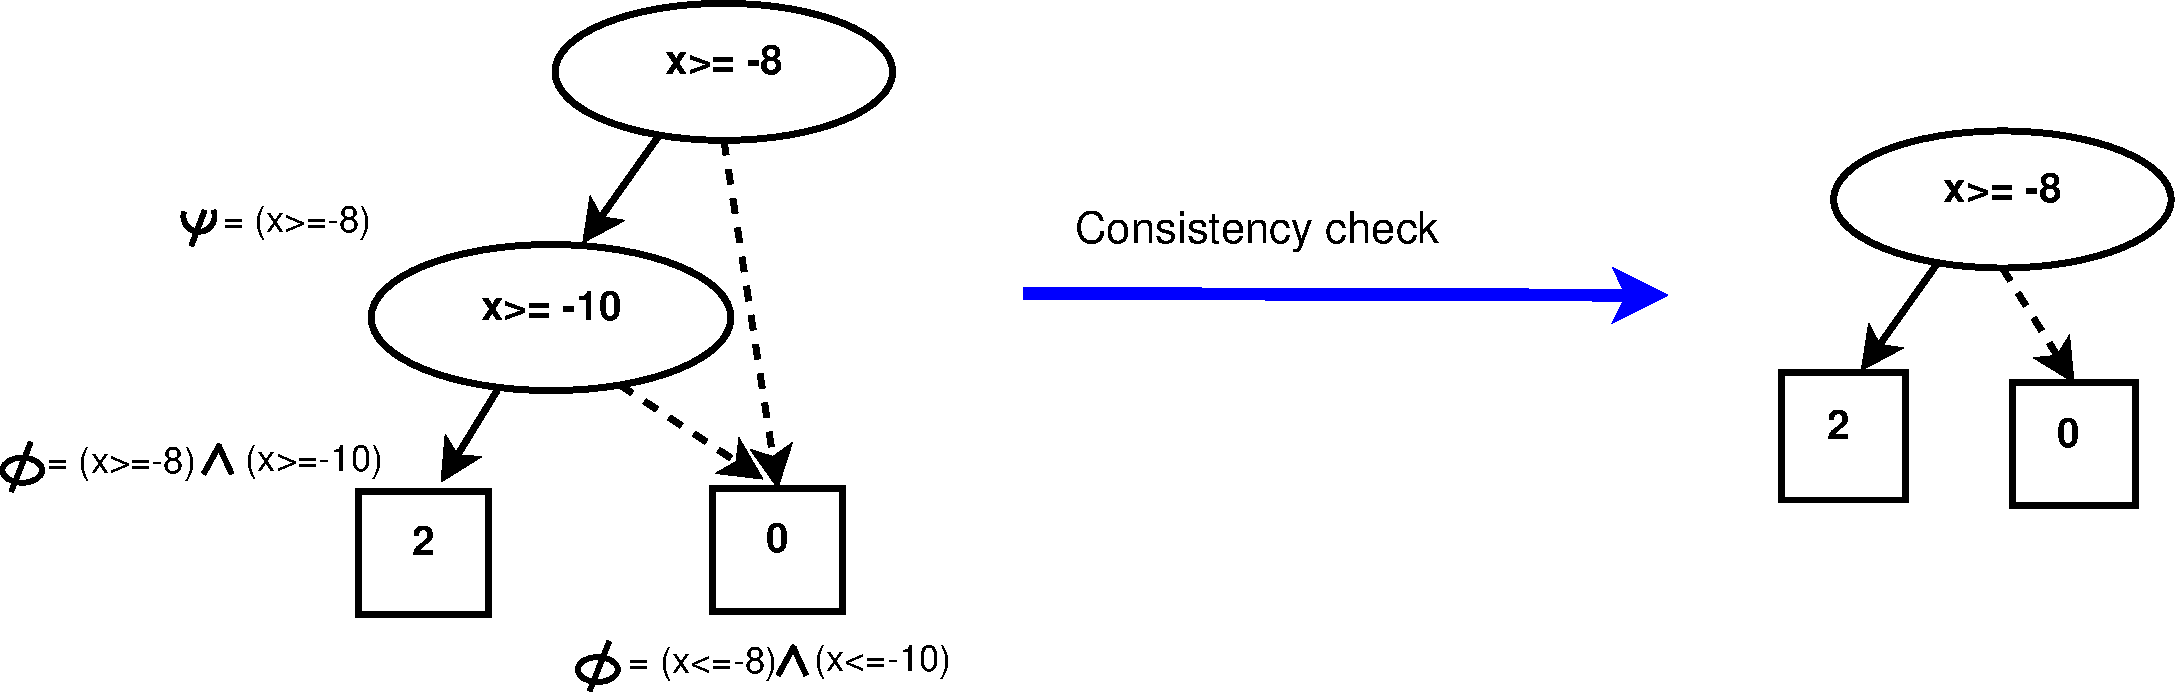
\includegraphics[width=0.9\textwidth]{pics/pruningC.pdf}
%\vspace{-3mm}
%\hspace{1mm}
%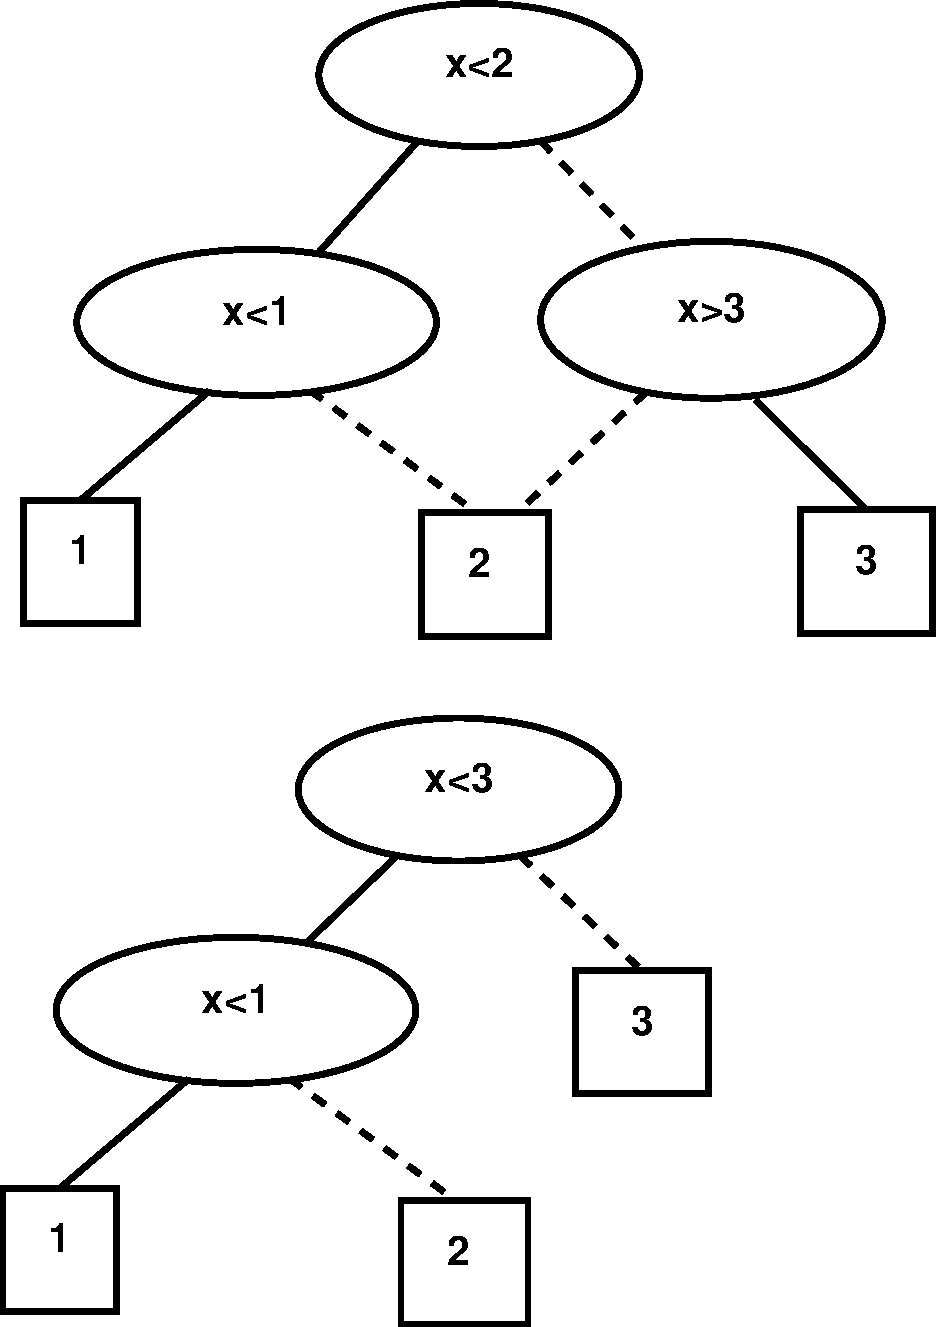
\includegraphics[width=0.18\textwidth]{xaddFig/counterexample.pdf}
\vspace{-2mm}
\caption{%\footnotesize 
{\it (left)} Path definitions on each node in the XADD with an inconsistent path $(x \geq -8) \wedge (x \geq -10 \models\perp)$; {\it (right)} Pruned XADD after removing unreachable node $x \geq -10$.}
\label{fig:consistent_graph}
%\vspace{-4mm}
\end{figure}
%%%%%%%%%%%%%%%%%%%%%%%%%%%%%%%%%%%%%%%%%%%%%%%%%%%%%%%%%%
\begin{mydef}(\textbf{Path}):
A path in an XADD $F$ is defined as the conjunction of decision tests and their value from root to node $i$, that is $P_j^i = \lbrace (dec_k, \rho(dec_k)\rbrace$ where $j$ denotes the path number. 
The path leading to node $F_i$ is defined by the conjunction of all decision nodes $F_k$ (and their assignments) occurring before $F_i$ in XADD $F$. The formula for such a path $P_1^i$ is represented below:

\begin{equation}
\psi_j^{i} := \bigwedge_{k=1}^{i-1}
\begin{cases}
\rho(\mathit{dec}_k) = \mathit{true}: & \mathit{dec}_k\\ 
\rho(\mathit{dec}_k) = \mathit{false}: & \neg \mathit{dec}_k \\ 
\end{cases}. \label{eq:path}%), (F_2,\rho(F_2)), \cdots, (F_i,\rho(F_i)) \rangle
\end{equation}
\end{mydef}

Recall the leaf node $F_i$ has the value $f_i$ in the case representation of Equation~\ref{eq:function_xadd}. We can now formally define a \emph{case partition} 
$\langle \phi_i(\vec{b},\vec{x}): f_i(\vec{x})\rangle$ using the path definition in~\ref{eq:path}: 

\begin{mydef}(\textbf{Case Partition}):
The disjunction of all paths $\psi^i$ from root to leaf node $F_i$, denoted by $\phi^i$, is defined below: 
\begin{equation}
\phi_j := \bigvee_{j=1}^{d} \psi_j^{i} \label{eq:casePartition}
\end{equation} 
where $1 \leq j \leq d$ is the number of paths $\psi_j^i$ leading to leaf node $F_i$.
\end{mydef}
Figures~\ref{fig:consistent_graph} and~\ref{fig:redundant_graph} show two XADDs with all $\psi$ and $\phi$ paths before applying pruning techniques. 
%%%%%%%%%%%%%%%%%%%%%%%%%%%%%%%%%%%%%%%%%%%%%%%%%%%%%%%%%%%%%%%%%%%%%%%%%%
\begin{figure}[t!]
\centering
%\subfigure{
%\hspace{-20mm}
%\vspace{-3mm}
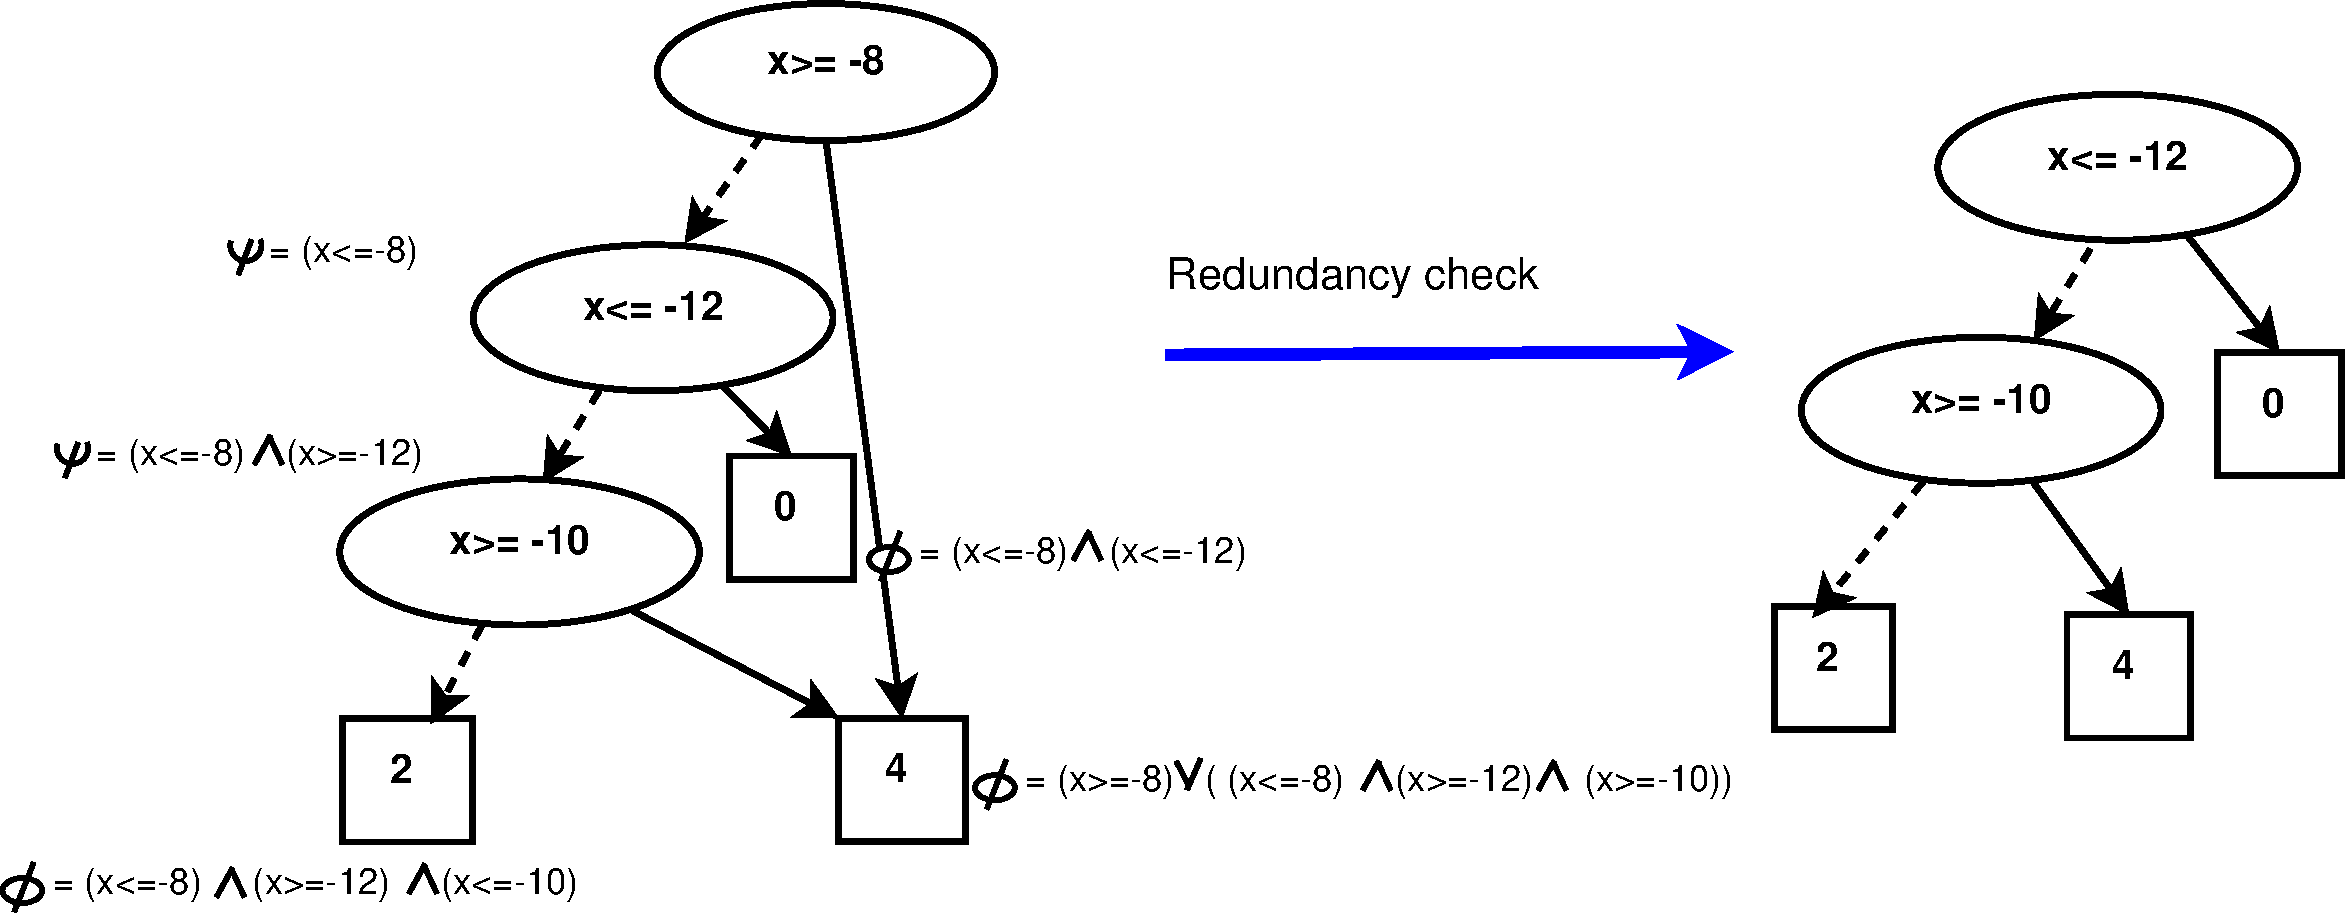
\includegraphics[width=0.9\textwidth]{pics/pruningR.pdf}
%\vspace{-3mm}
%\hspace{1mm}
%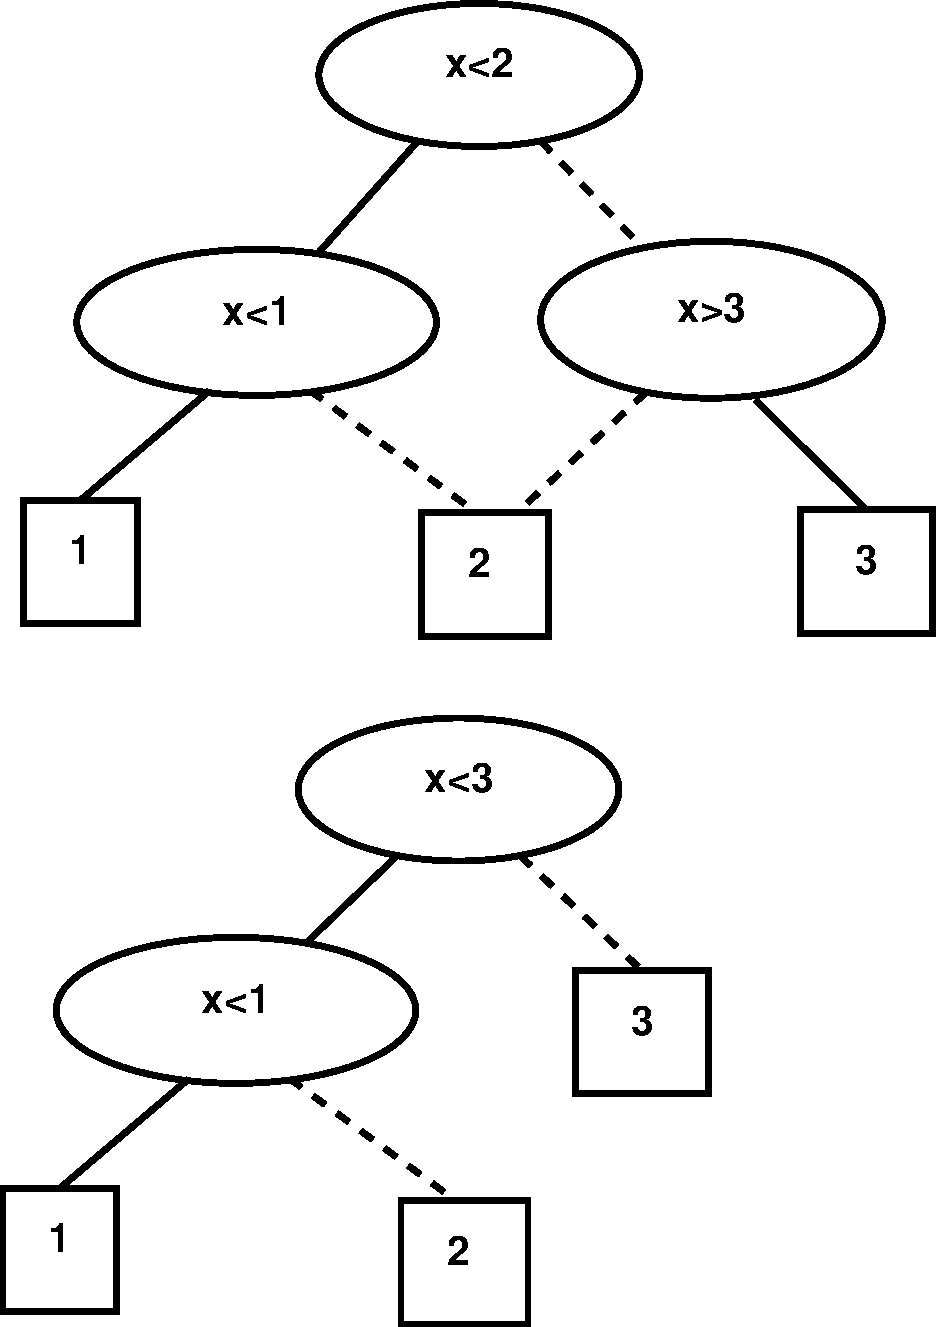
\includegraphics[width=0.18\textwidth]{xaddFig/counterexample.pdf}
\vspace{-2mm}
\caption{%\footnotesize 
{\it (left)} Path definitions on each node in the XADD with the redundant nodes of $x>=-8$; since it is redundant in the paths leading to leaf node $4$, that is:  $(x \geq -8) \vee ((x \leq -8)\wedge(x \geq -12)\wedge(x \geq -10)) \equiv (x \geq -12)\wedge(x \geq -10)$;{\it (right)} The pruned XADD without the redundant node.}
\label{fig:redundant_graph}
%\vspace{-4mm}
\end{figure}
%%%%%%%%%%%%%%%%%%%%%%%%%%%%%%%%%%%%%%%%%%%%%%%%%%%%%%%%%%
According to the definitions of~\ref{eq:path} and~\ref{eq:casePartition}, we can now define an inconsistent path as the following: 

\begin{mydef}(\textbf{Inconsistent path}):
A path $\psi_i$ in XADD $F$ is inconsistent if $\psi_i \models \perp$.
An unreachable node is the final decision node on this inconsistent path by any assignment to $(\vec{b},\vec{x})$. In the next section we describe how to prune such nodes from the XADD.
As an example, Figure~\ref{fig:consistent_graph} (left) has an inconsistent path on which $x \geq -10$ violates the previous constraint of $x\geq -8$, that is: $(x \geq -8) \wedge (x \geq -10 \models\perp$. The XADD never reaches beyond $x \geq -10$, making it an unreachable node.
\end{mydef}

Removing redundant nodes or branches from the XADD is a requirement for obtaining a compact XADD representation. Redundant low and high branches are easy to detect for any node and can be removed from an XADD using Algorithm \ref{algGetNode} presented in the next section. A redundant node occurs in an XADD where two nodes give the same function definition and removing one does not change any of the partitions of that function. As an example consider the left diagram of Figure~\ref{fig:redundant_graph}. Here removing node $x>=-8$ will not effect the function of final XADD as presented on the right side. The following provides a definition of redundancy in XADD nodes:  
\begin{mydef}(\textbf{Redundant node}):
A node $F_r$ in $\phi_j^i$ is redundant if removing its decision constraint $\mathit{dec}_r$ in any of the paths containing $F_r$ does not change this case partition. Upon removing a decision constraint either the $\mathit{true}$ or $\mathit{false}$ branch is taken. Therefore a boolean assignment to $\mathit{dec}_r$ in $\phi_j^i$ (i.e. that is the assignment of [$\rho(\mathit{dec}_r) \rightarrow \mathit{true}$] or [$\rho(\mathit{dec}_r) \rightarrow \mathit{false}$])
must equal the set of paths minus node $F_r$. 

Consider Figure~\ref{fig:redundant_graph} (left) at the leaf node with value $4$. The set of all paths for this node is equal to $\phi_4 = (x \geq -8) \vee ((x \leq -8)\wedge(x \geq -12)\wedge(x \geq -10))$ which is equal to $(x \geq -12)\wedge(x \geq -10)$; thus removing the redundant node of decision $(x \geq -8)$ results in the right-most figure.
\end{mydef}
%%%%%%%%%%%%%%%%%%%%%%%%%%%%%%%%%%%%%%%%%%%%%%%%%%%%%%%%%%%%%%%%%%%%%%%%%%%%
%\vspace{10mm}
\begin{figure}[t!]
\centering
%\subfigure{
%\hspace{-20mm}
%\vspace{-3mm}
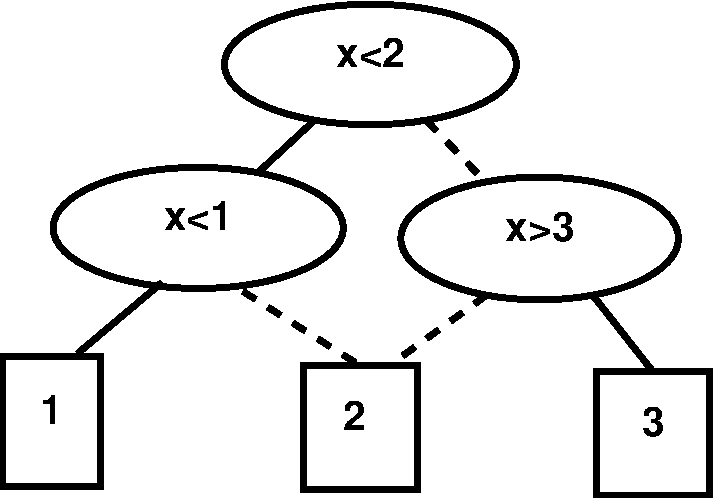
\includegraphics[width=0.25\textwidth]{pics/counterexample1.pdf} 
\hspace{20mm}
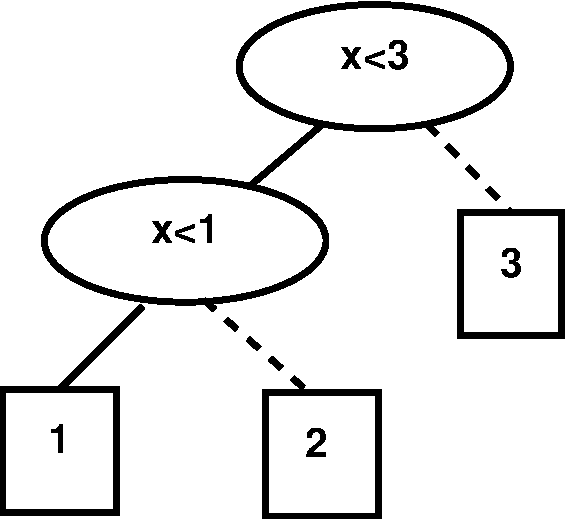
\includegraphics[width=0.20\textwidth]{pics/counterexample2.pdf} 
%\includegraphics[width=0.62\textwidth]{xaddFig/redundancy_proof.pdf}
\caption{%\footnotesize 
{\it (left)} A counterexample for an XADD that is not canonical after applying consistency and redundancy checking; {\it (right)}  The true value of the true XADD which can not be derived from the left diagram.} %{\it (right)} Example of removing the redundant node $i$ which must result in an equal XADD from root up to node $i$ branched on the true or false branch of $dec_i$. }
\label{fig:canonical}
%\vspace{-6mm}
\end{figure}
%%%%%%%%%%%%%%%%%%%%%%%%%%%%%%%%%%%%%%%%%%%%%%%%%%%%%%%%%%%%%%%
%%%added after taking canonical proof out
It seems that using the two mentioned pruning techniques of inconsistency and redundancy checking removes all sources of infeasibility and therefore proof of canonicity is straightforward. Indeed for BDDs and ADDs proof of canonicity can be defined using the reduced diagrams (\cite{bryant}). 
As we defined reduced XADDs are derived from the result of the applying redundant branch pruning. Furthermore two pruning techniques of inconsistent path checking and redundant node pruning are applied to the final result of all XADDs. However unlike BDDs and ADDs a canonical XADD may not be produced after such pruning approaches. As a counterexample consider the simple XADD in the top left diagram of Figure~\ref{fig:canonical} where the values as below: 
\begin{align*}
	\begin{cases}
		x \leq 1 :& 1  \\
		x \geq 3 :&3\\
		1<x<3 :& 2\\
	\end{cases}
\end{align*}
As the values suggest, there is no need to branch on $x<2$ in this function, i.e. it can be removed from the tree. According to the implication checks in both pruning techniques, this XADD is not inconsistent and further it can not be removed using the redundant technique which replaces a redundant node with one of its branches. To remove the node, a \emph{reordering} of the decision nodes is required which will effect the structure of the tree, changing it to a new XADD. For this reason, although consistency and redundancy checking takes care of most unwanted branches, there is no guarantee that a given XADD is minimal after applying the two pruning techniques. The right diagram of Figure~\ref{fig:canonical} is the true value this XADD holds which is a different XADD. Thus a challenging open problem is the proof of XADD minimality with respect to a reordering for linear decision nodes. 

In the next section we use the definitions of inconsistency and redundancy to provide efficient algorithms to prune XADDs. 

\subsection{XADD Algorithms}
\label{sec:pruningAlg}
%%%%%%%%%%%%%%%%%%%%%%%%%%%%%%%%%%%%%%%%%%%%%%%%%%%%%%%%%%%%%%%%%
\incmargin{.5em}
\begin{algorithm}[t!]
\SetKwInOut{Input}{input}
\SetKwInOut{Output}{output}
\dontprintsemicolon
\Begin{
   //redundant branches\\
   \If{$F_l = F_h$}
   {
      \Return{$F_l$}\;
   }
   //check if the node exists previously\\
   \If{$\langle \mathit{dec}, F_h, F_l \rangle \rightarrow \mathit{id}$ is not
   in NodeCache}
   {id\ = new unallocated id\;  
    insert $\langle \mathit{dec}, F_h, F_l \rangle \rightarrow \mathit{id}$ in NodeCache\;
   }
   \Return{id}\;
}
\caption{{\sc GetNode}($\mathit{dec}, F_h, F_l$) $\longrightarrow \langle F_r \rangle$\label{algGetNode}}
\end{algorithm}
\decmargin{.5em}
%%%%%%%%%%%%%%%%%%%%%%%%%%%%%%%%%%%%%%%%%%%%%%%%%%%%%%%%%%%%%%%%
Before defining our pruning algorithms, we first describe how a reduced XADD can be constructed from an arbitrary ordered decision diagram represented by $\lbrace 0,1 \rbrace^m \times \mathbb{R}^{n} \rightarrow \mathbb{R}$.

The helper function \emph{getNode} in Algorithm \ref{algGetNode} is used in all future algorithms. This algorithm returns a compact representation of a single internal decision node. It checks for branch redundancy so that no node has identical children on the high and low branch. If a redundant branch is found, it simply returns one of the children nodes in lines 3--4. Otherwise this function must build a new node with a unique id. Each new id is stored in a  \emph{NodeCache} table and lines 6--8 shows that before adding a new node, the cache is checked for an existing node with the same properties. 

Algorithm \emph{ReduceXADD} allows the construction of a compact XADD representation for a given XADD. This algorithm recursively constructs a reduced XADD from the bottom up. 
If the root node input to the algorithm is a leaf node, the algorithm returns the canonical form of $F$ in lines 4--5. Note that for a linear expression in the leaf, the canonical form is $c_0+\sum_{i} c_i x_i , 0 \leq i \leq n$, however for arbitrary functions finding a canonical form may be time consuming or intractable. 

If the root node input to the algorithm is a decision node then lines 7--13 are executed. A decision node is represented as $\langle \mathit{dec}, F_h, F_l \rangle$, where $\mathit{dec}$ is the variable name, and $F_h$ and $F_l$ are the id for high and low branches respectively. The algorithm recursively computes the reduced XADDs of the low and high branch. It then uses the \emph{GetNode} function in Algorithm~\ref{algGetNode} to remove any redundant branch. 
%Paths are checked for inconsistency in line 12 which performs the forthcoming Algorithm~\ref{algPrune} and the $\mathit{true}$ parameter also allows checking for redundant nodes. 
Reduced XADDs rooted at $F_r$ are then stored in the \emph{ReduceCache} table. \emph{ReduceCache} ensures that each node is visited once and a unique reduced node is generated in the final diagram. Thus \emph{ReduceXADD} has linear running time according to the number of nodes in $F_r$.
%%%%%%%%%%%%%%%%%%%%%%%%%%%%%%%%%%%%%%%%%%%%%%%%%%%%%%%%%%%%%%%%%
\incmargin{.5em}
\linesnumbered
\begin{algorithm}[t!]
\SetKwFunction{getNode}{{\sc GetNode}}
\SetKwFunction{reduce}{{\sc ReduceXADD}}
\SetKwFunction{redundant}{{\sc PruneRedundancy}}
\SetKwInOut{Input}{input}
\SetKwInOut{Output}{output}
\dontprintsemicolon
%\Input{$F$ (root node id for an arbitrary ordered decision diagram)}
%\Output{$F_r$ (root node id for reduced XADD)}
%\BlankLine
\Begin{
   //F is root node id for an arbitrary ordered decision diagram\\
   //$F_r$ is root node id for a reduced XADD\\
   \If{F is terminal node}
   {
   \Return{canonical terminal node for $F$}\;
   }
   //else reduce decision node $\mathit{dec}$\\
   \If{$F \rightarrow F_r$ is not in ReduceCache}
   {
    $F_h$ = \reduce{$F_h$}\;
    $F_l$ = \reduce{$F_l$}\;
    //get a canonical internal node id\\
    $F_r$ = \getNode{$\mathit{dec}$, $F_h$, $F_l$}\;
    %$F_r = $ \redundant{$F$, $\psi$,$\mathit{true}$}\;
    insert $F \rightarrow F_r$ in ReduceCache\;
   } 
   \Return{$F_r$}\;
}
\caption{{\sc ReduceXADD}($F$) $\longrightarrow$ $\langle F_r \rangle$ \label{algReduceXADD}}
\end{algorithm}
\decmargin{.5em}
%%%%%%%%%%%%%%%%%%%%%%%%%%%%%%%%%%%%%%%%%%%%%%%%%%%%%%%%%%%%%%%%%

Given a reduced XADD with no redundant branches, we further prune inconsistent paths and redundant nodes in the following sections.
%%%%%%%%%%%%%%%%%%%%%%%%%%%%%%%%%%%%%%%%%%%%%%%%%%%%%%%%%%%%%%%%
\incmargin{.5em}
\linesnumbered
\begin{algorithm}[t!]
\SetKwFunction{getNode}{{\sc GetNode}}
\SetKwFunction{testImplied}{{\sc TestImplied}}
\SetKwFunction{prune}{{\sc PruneInconsistent}}
\SetKwFunction{redundant}{{\sc IsRedundant}}
\SetKwInOut{Input}{input}
\SetKwInOut{Output}{output}
\dontprintsemicolon
%\Output{$F_r$ (root node id for a consistent XADD)}
\BlankLine
\Begin{
    //$F$ is the root node represented as ($\mathit{dec},F_l,F_r$)\\
    %//$\psi$ is the set of decision constraints\\
   \If{$F$ is terminal node}
   {
    \Return{canonical terminal node for $F$}\;
   }
   //if $F$ is a boolean decision, no inconsistency checking possible for $F$\\
   \If {$F \in \lbrace 0,1 \rbrace^m$}
   {
    $low =$  \prune{$F_l$, $\psi$}\;
    $high =$  \prune{$F_h$, $\psi$}\;	
    \Return  {\getNode{$\mathit{dec},high,low$}}\; 
   }
   //else $F$ is a linear decision check if  $\psi\models\perp$\\
   
    	 \If{\testImplied{$\psi$,$\mathit{dec}$}}
    			{ \Return { \prune{$F_h$, $\psi$}}\;}
    	 \If{\testImplied{$\psi$,$\neg\mathit{dec}$}}
    			{\Return { \prune{$F_l$, $\psi$}}\;}
  //result of TestImplied was false\\
	
     $\psi \longleftarrow \left[ \psi,\neg \mathit{dec} \right]$\;
    $low=$  \prune{$F_l$, $\psi$}\;
    $\psi \longleftarrow  \psi \setminus \neg \mathit{dec} $\;
     $\psi \longleftarrow \left[ \psi,\mathit{dec} \right]$\;
    $high=$  \prune{$F_h$, $\psi$}\;	 
    $\psi \longleftarrow \psi \setminus \mathit{dec} $\;
     \If {$\mathit{testRedundant}$}
    {
	 //check if high branch is implied in the low branch\\
     $\psi \longleftarrow \left[ \psi,\mathit{dec} \right]$\;
     $\mathit{isRedundant} = $\redundant{$\psi$,$low$, $high$}\;
      $\psi \longleftarrow \psi \setminus \mathit{dec} $\;
     \If {$\mathit{isRedundant}$}
    {\Return{$low$}\;}     
	//is low branch implied in the high branch for the negation of $\mathit{dec}$\\
	 $\psi \longleftarrow \left[ \psi,\neg \mathit{dec} \right]$\;
     $\mathit{isRedundant} = $\redundant{$\psi$,$high$, $low$}\;
    $\psi \longleftarrow  \psi \setminus \neg \mathit{dec} $\;
   \If {$\mathit{isRedundant}$}
    {\Return{$high$}\;}     
	}     
    
    \Return{$F_r=$ \getNode{$\mathit{dec},high,low$}}\;
}
\caption{{\sc PruneInconsistent}($F$, $\psi$,$\mathit{testRedundant}$) $\longrightarrow$ $\langle F_r \rangle$ \label{algPrune}}
\end{algorithm}
\decmargin{.5em}
%%%%%%%%%%%%%%%%%%%%%%%%%%%%%%%%%%%%%%%%%%%%%%%%%%%%%%%%%%%%%%%%%
\subsubsection{Inconsistency Pruning Algorithm}
Given an XADD $F$ with potential inconsistent paths and the set of decision constraints on a path $\psi$, the output of \emph{PruneInconsistent} (Algorithm~\ref{algPrune}) is a reduced XADD with canonical leaves, linear decisions and no unreachable nodes. Similar to Algorithm \emph{ReduceXADD}, this algorithm is of a recursive bottom-up nature. 

Lines 3--4 returns a canonical linear expression at the leaf if $F$ is a terminal node. Since $F$ does not require path consistency checking at a boolean decision node, lines 6--9 recursively calls inconsistency pruning on the low and high branches. The final result is returned using Algorithm~\ref{algGetNode}.

If the two mentioned conditions are false, then the current node of $F$ is a linear decision node. Here we check if the decision constraint of this node ($\mathit{dec}$) is consistent with the previous constraints on path $\psi$. 
Lines 11 and 13 use the \emph{TestImplied} function which performs the following steps. The input to this algorithm is the path $\psi$ and current decision node constraint $\mathit{dec}$. 
\begin{itemize}
\item Check if the implication result of $\psi$ exists in an \emph{Implications} cache. This cache stores paths $\psi$ that are inconsistent. If there is a previous result which already contains the new decision constraint $\mathit{dec}$ then return $\mathit{true}$.
\item Similarly check the \emph{non-Implications} cache for consistent path $\psi$. If there is a previous result which already contains the new decision constraint $\mathit{dec}$ then return $\mathit{false}$.
\item If there is no cache hit, then the negation of $\mathit{dec}$ is added to the path: $\psi \longleftarrow \left[ \psi, \neg \mathit{dec} \right]$. This allows us to check for the infeasibility property.
\item The LP-solver is called on the set of decision constraints in $\psi$. The result of the LP-solver determines infeasibility with respect to the new decision added to $\psi$, which is implementing inconsistency checking. 
\item The path $\psi$ is stored in its related cache according to the result of the LP-solver (i.e. $\mathit{true}$ or $\mathit{false}$). If the result is inconsistent then $\psi$ is added to \emph{Implications}, else it is added to \emph{non-Implications}.
\item The negation of $\mathit{dec}$ is removed from the path: $\psi \longleftarrow \psi \setminus \neg \mathit{dec}$.
\item The result of the LP-solver is returned as the output of this function.
\end{itemize}
Line 11 checks for the high branch of $F$ that is adding the true assignment of $\mathit{dec}$. If $\mathit{true}$ is returned from \emph{TestImplied}, then the high branch is inconsistent. As a result this algorithm returns the child at the high branch as the result of this pruning in line 12. Similarly in line 13 the low branch is checked with  $\neg \mathit{dec}$ and if $\mathit{true}$ is returned then the low branch is inconsistent and line 14 is returned.

In case the current decision node is not on an inconsistent path, both low and high branches need to be checked for inconsistency. Lines 17--19 add the decision constraint for the low branch $\neg \mathit{dec}$ to $\psi$ and call \emph{PruneInconsistent} for $F_l$ and removes this constraint after this call. Lines 20--22 perform the same for the high branch ($F_h$). 

At this stage the current subtree with the computed low and high branches does not contain any inconsistent paths. Thus if the boolean indicator to check for redundancy $\mathit{testRedundant}$ is set to $\mathit{false}$ then this algorithm returns a reduced node computed using \emph{GetNode} in line 37. However as we explain in the next section, for full pruning (i.e. $\mathit{testRedundant}= \mathit{true}$) all redundant nodes must be pruned.
%%%%%%%%%%%%%%%%%%%%%%%%%%%%%%%%%%%%%%%%%%%%%%%%%%%%%%%%%%%%%%%%%
\incmargin{.5em}
\linesnumbered
\begin{algorithm}[t!]
\SetKwFunction{getNode}{{\sc GetNode}}
\SetKwFunction{testImplied}{{\sc TestImplied}}
\SetKwFunction{prune}{{\sc IsRedundant}}
\SetKwInOut{Input}{input}
\SetKwInOut{Output}{output}
\dontprintsemicolon
%\Input{$X$ (root node id for a consistent XADD), $KB$ (child-parent implications), $F$ (formulas for each node)}
\BlankLine
\Begin{
	//both branches are terminal nodes, redundant if high=low\\
   \If{$\mathit{subtree} = \mathit{goal}$}
   {
    \Return{$\mathit{true}$}\;
   }
   \If{$\mathit{subtree}$ is non-terminal node}
   {
   	   \If{$\mathit{goal}$ is non-terminal node}
       {
    	   //node is not redundant if the goal occurs before subtree\\
    	   \If{$\mathit{subtree} \geq \mathit{goal}$}
    	    {
   				 \Return{$\mathit{false}$}\;
   			}
       }
       	// check if $\mathit{subtree} \models \mathit{goal}$\\
        \If{\testImplied{$\psi$,$\neg \mathit{subtree}_{\mathit{dec}}$}}
    			{ \Return { \prune{$\psi$,$\mathit{subtree}_l$ ,$\mathit{goal}$}}\;}
    	 \If{\testImplied{$\psi$,$\mathit{subtree}_{\mathit{dec}}$}}
    			{\Return { \prune{$\psi$,$\mathit{subtree}_h$ ,$\mathit{goal}$}}\;}
      
      //result of TestImplied was false\\
     $\psi \longleftarrow \left[ \psi,\neg \mathit{subtree}_{\mathit{dec}}\right]$\;
    $\mathit{isImplied}=$  \prune{$\psi$,$\mathit{subtree}_l$ ,$\mathit{goal}$}\;
    $\psi \longleftarrow  \psi \setminus \neg \mathit{subtree}_{\mathit{dec}} $\;
    //if the low branch does not imply goal, the node is not redundant\\
     \If{$\neg \mathit{isImplied}$}
    	    {
   				 \Return{$\mathit{false}$}\;
   			}
     $\psi \longleftarrow \left[ \psi,\mathit{subtree}_{\mathit{dec}} \right]$\;
    $\mathit{isImplied}=$  \prune{$\psi$,$\mathit{subtree}_h$ ,$\mathit{goal}$}\;
    $\psi \longleftarrow \psi \setminus \mathit{subtree}_{\mathit{dec}} $\;	
    \Return{$\mathit{isImplied}$}\;		
   }
   \Return{$\mathit{false}$}\;
}
\caption{{\sc IsRedundant}($\psi$, $\mathit{subtree}$, $\mathit{goal}$) $\longrightarrow$ $\langle F_r \rangle$ \label{algRedundant}}
\end{algorithm}
\decmargin{.5em}
%%%%%%%%%%%%%%%%%%%%%%%%%%%%%%%%%%%%%%%%%%%%%%%%%%%%%%%%%%%%%%%%%
\subsubsection{Redundancy Pruning Algorithm}

Lines 22--34 of Algorithm~\ref{algPrune} removes any redundant nodes from the subtree rooted at $\langle \mathit{dec}, low, high \rangle$ where $low$ and $high$ are the subtrees after inconsistent pruning. To check for redundancy, the decision constraint of the current subtree is added to $\psi$ and a call is made to Algorithm~\ref{algRedundant}. Intuitively \emph{IsRedundant} checks to see whether a $\mathit{subtree}$ can replace another subtree $\mathit{goal}$ without changing the XADD function. 

Initially lines 3--4 check if  $\mathit{subtree}$ and $\mathit{goal}$ are terminal nodes and equal, in this case the $\mathit{goal}$ is redundant and can be replaced by $\mathit{subtree}$, therefore the algorithm returns $\mathit{true}$. If the nodes are non-equal terminal nodes then $\mathit{goal}$ is not redundant and line 28 returns $\mathit{false}$. Next lines 6--9 check if both nodes are decision nodes but the $\mathit{goal}$ node appears before the $\mathit{subtree}$ in the variable ordering of the XADD, in which case the $\mathit{goal}$ subtree can not be redundant. 

If neither of the above cases occur, the algorithm must check whether $\mathit{subtree} \models \mathit{goal}$ using the  \emph{TestImplied} function. Lines 11--15 call \emph{TestImplied} for the decision constraint of the root node of $\mathit{subtree}$. If  \emph{TestImplied} returns $\mathit{true}$ for the false value of the decision node (i.e. $\mathit{subtree}_{\mathit{dec}}$), then the algorithm returns the redundancy check for the low child of the $\mathit{subtree}$. For the true value of $\mathit{subtree}_{\mathit{dec}}$ a recursive call to \emph{IsRedundant} is performed with the high child. This process ensures that the entire subtree is traversed and all children of the subtree also imply the $\mathit{goal}$. 

Similar to Algorithm~\ref{algPrune}, if the result of \emph{TestImplied} is false, both low and high branches need to be checked for redundancy. Lines 18--20 adds the decision constraint for the low branch $\neg \mathit{subtree}_{\mathit{dec}}$ to $\psi$ and calls \emph{IsRedundant} for $\mathit{subtree}_l$ and removes this constraint after this call. If any of the children along the way do not imply $\mathit{goal}$, then $\mathit{goal}$ can not be considered redundant as line 22--23 illustrates. 
Lines 24--27 perform the same for the high branch $\mathit{subtree}_h$ and returns the result of \emph{IsRedundant}.

Returning back to Algorithm~\ref{algPrune}, line 26 removes the current decision constraint from $\psi$ and checks for redundant nodes returned from Algorithm~\ref{algRedundant}. If the algorithm has returned $\mathit{true}$ then the low branch is sufficient to represent this subtree, as the node in the high branch is redundant. Figure~\ref{fig:redundant_graph}(right) shows that the node $x\geq -8$ in the left figure is redundant and can be removed from the diagram. 

A similar approach is then performed in lines 29--34 to check if the $low$ branch is implied in the $high$ branch given the decision constraint is $\mathit{false}$. In this case the $high$ branch is returned instead of the node rooted at $\mathit{dec}$. This concludes the pruning algorithm for removing any redundant node from the XADD $F$. 

Next we present the main XADD operations required for SDP algorithms.

\subsection{XADD Operations}
\label{sec:xaddoperations}
In this section we review the symbolic operations required to perform SDP using the XADD structure. This is mainly categorized into unary and binary operations.   
\subsubsection{Unary XADD Operations}
%%%%%%%%%%%%%%%%%%%%%%%%%%%%%%%%%%%%%%%%%%%%%%%%%%%%%%%%%%%%%%%%%%%%%%%%%%%%
%\vspace{10mm}
\begin{figure}[t!]
\centering
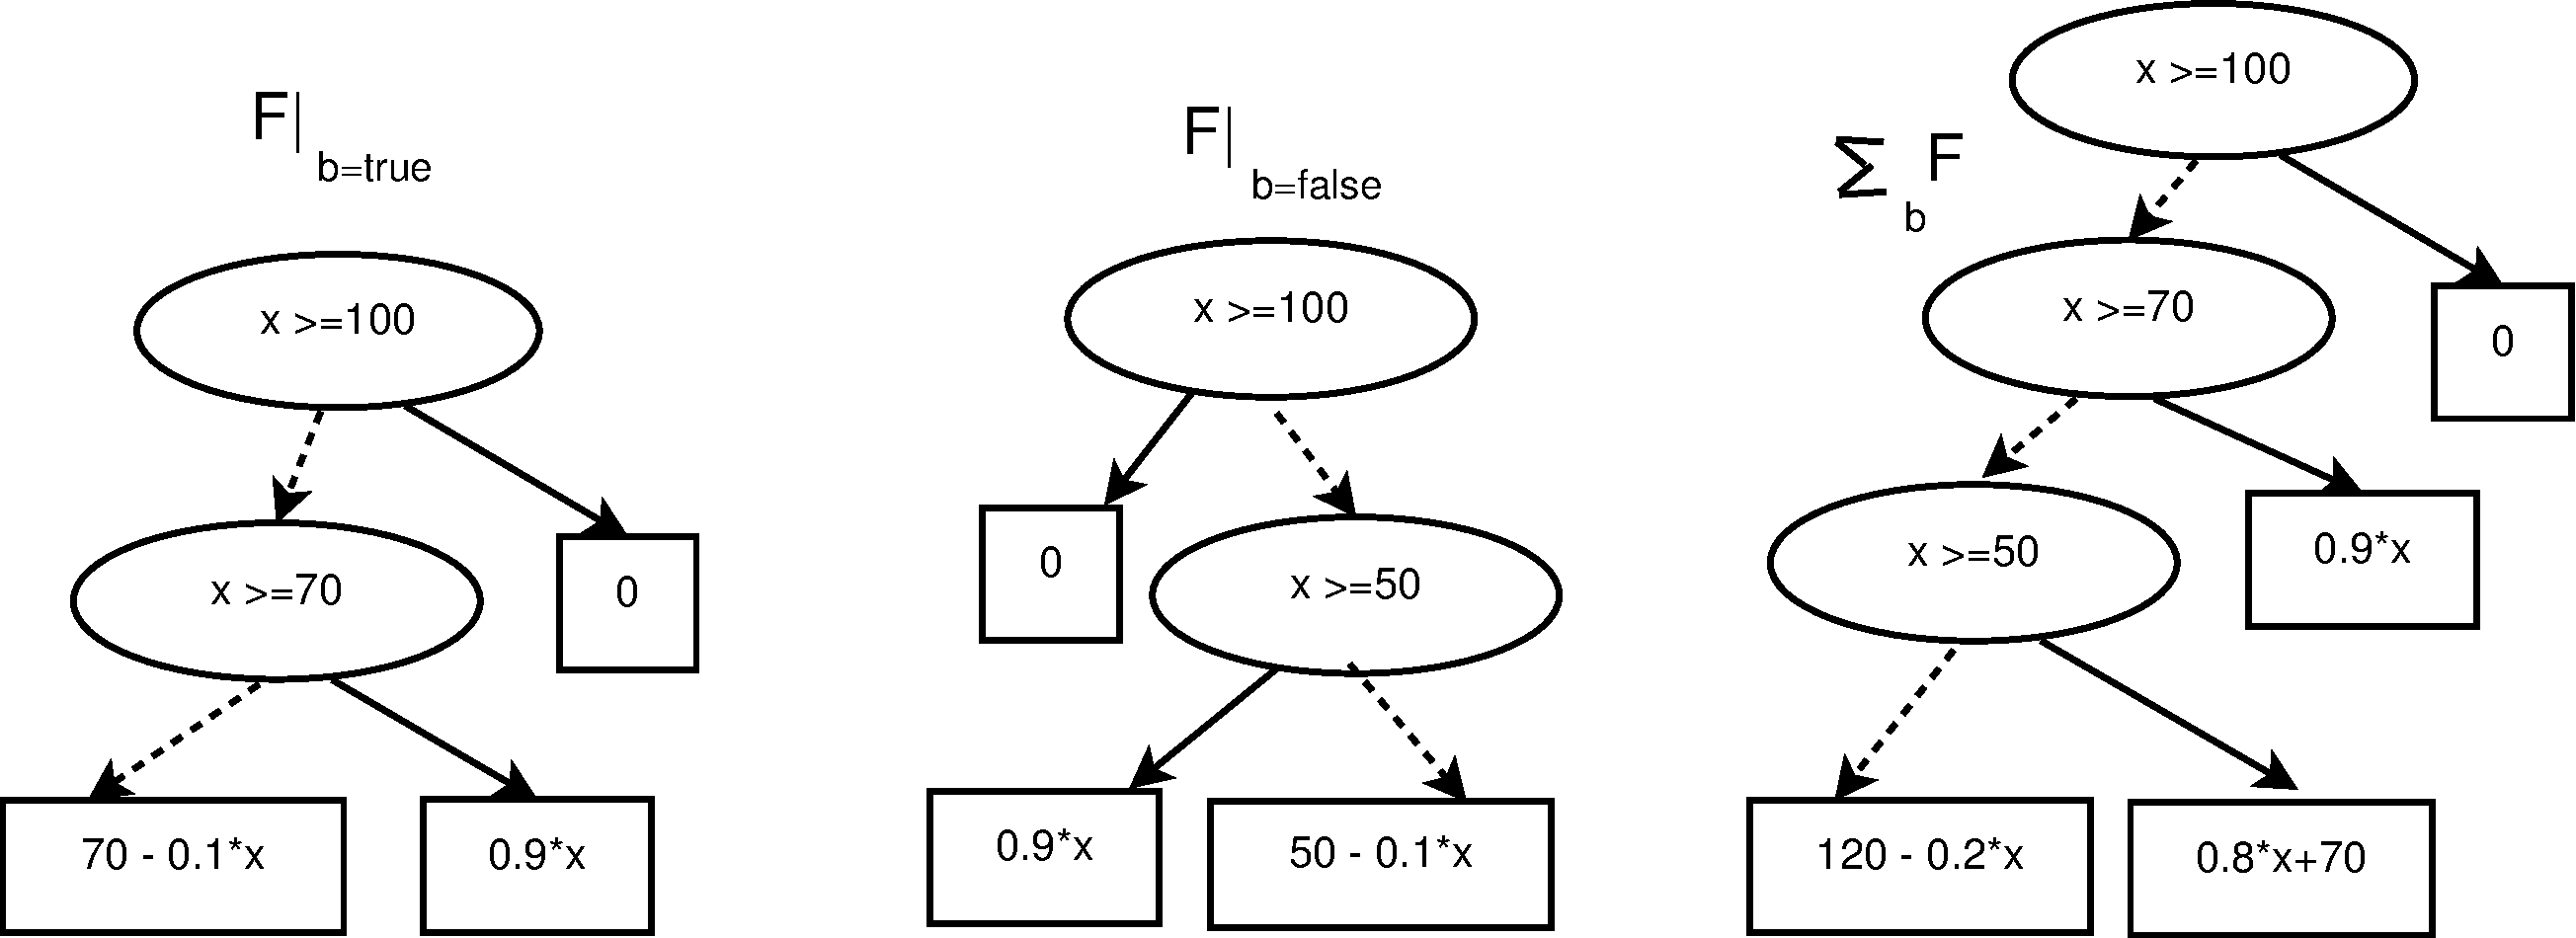
\includegraphics[width=0.85\textwidth]{pics/restriction.pdf}
%\vspace{-2mm}

\caption{%\footnotesize 
{\it (left)} Example of restriction operation $F|_{b=true}$ and $F|_{b=false}$ on the XADD of Figure~\ref{fig:bdd_add_xadd}(right) for the binary variable $b$. {\it (right)} The resulting XADD after marginalization $\sum_{b}F$.}
\label{fig:restrict}
%\vspace{-6mm}
\end{figure}
%%%%%%%%%%%%%%%%%%%%%%%%%%%%%%%%%%%%%%%%%%%%%%%%%%%%%%%%%%%%%%%
%%%%%%%%%%%%%%%%%%%%%%%%%%%%%%%%%%%%%%%%%%%%%%%%%%%%%%%%%%%%%%%%%
\incmargin{0.5em}
\linesnumbered
\begin{algorithm}[t!]
\SetKwFunction{getCanonicalNode}{{\sc GetCanonicalNode}}
\SetKwFunction{reduce}{{\sc Reorder}}
\SetKwInOut{Input}{input}
\SetKwInOut{Output}{output}
\dontprintsemicolon

%\Input{$F$ (root node for possibly unordered XADD)}
%\Output{$F_r$ (root node for an ordered XADD)}
\BlankLine
\Begin{
   \If{F is terminal node}
   {
   \Return{canonical terminal node of $F$}\;
   }
   \If{$F \rightarrow F_r$ is not in ReorderCache}
   {
    $F_{\mathit{true}}$ = \reduce{$F_{\mathit{true}}$} $\otimes \; \mathbb{I}[\mathit{dec}]$ \;
    $F_{\mathit{false}}$ = \reduce{$F_{\mathit{false}}$} $\otimes \; \mathbb{I}[\neg \mathit{dec}]$\;
    $F_r = F_{\mathit{true}} \oplus F_{\mathit{false}}$\;
    insert $F \rightarrow F_r$ in ReorderCache\;
   } 
   \Return{$F_r$}\;
}
\caption{{\sc Reorder}($F$) $\longrightarrow$ $\langle F_r \rangle$ \label{alg:reorder}}
\end{algorithm}
\decmargin{0.5em}
%%%%%%%%%%%%%%%%%%%%%%%%%%%%%%%%%%%%%%%%%%%%%%%%%%%%%%%%%%%%%%%%%
According to the previous section on unary operations required in SDP, scalar multiplication $c.f$ and negation $- f$ on a function can simply be represented as an XADD. Negation of XADD $F$ is equal to performing a binary operation of $0 \ominus F$ explained in the next section. Furthermore restriction, substitution and integration of the $\delta$ function are also unary operations that can be applied to XADDs are explained below.  

Restriction of a variable $b$ in $F$ to some formula $\phi$ is performed by appending $\phi$ to each of the decision nodes (using logical $\wedge$) while leaves are not affected. For a binary variable, restriction is equal to taking the true or false branch that is ($F|_{b_i=true}$) or ($F|_{b_i=false}$). 
This operation can also be used for $\textit{marginalizing}$ boolean variables; $\sum_{b_i}$ eliminates variable $b_i$ from $F$  by computing the sum of functions restricted to \emph{true} or \emph{false} value of $b_i$, i.e. $F|_{b_i=true} \oplus \ F|_{b_i=false}$. The mentioned restriction operation uses $\oplus$ which is a binary operation handled in Algorithm~\ref{algApply}. Figure~\ref{fig:restrict} demonstrates restriction of $F|_{b}$ and the right diagram shows the marginalization of $\sum_{b}F$. 

Marginalizing a continuous variable $x$ is performed using the integration of the $\delta$-function on variable $x$. Specifically in SDP we require computing $\int_{x} \delta [ x - g(\vec{x})]fdx$ which triggers the substitution $f \lbrace x/ g(\vec{x})\rbrace$ on $f$ as defined next. Note that the XADD representation is used for both functions $f$ and $g$.
 
Substitution for a given XADD $F$ is performed by applying the set of variables and their substitutions to each case statement such that $\phi_i\sigma: f_i\sigma$. The substitution operand effects both leaves and decision nodes and changes them according to the variable substitute. 
Decisions may become unordered when substituted. A reorder algorithm has to be applied to the result of the substitution operand. As Algorithm~\ref{alg:reorder} shows, we recursively apply the binary operations of $\otimes$ and $\oplus$ to decision nodes for reordering the XADD after a substitution. Similar to other XADD algorithm a \emph{ReorderCache} is used to prevent unnecessary reordering. 

%%%%%%%%%%%%%%%%%%%%%%%%%%%%%%%%%%%%%%%%%%%%%%%%%%%%%%%%%%%%%%%%%
\incmargin{0.5em}
\linesnumbered
\begin{algorithm}[t!]
\dontprintsemicolon
\SetKwFunction{getRoots}{{\sc GetRoots}}
\SetKwFunction{reduce}{{\sc ReduceLinearize}}
\SetKwInOut{Input}{input}
\SetKwInOut{Output}{output}

%\Input{$F$ (root node id for an arbitrary ordered decision diagram)}
%\Output{$F_r$ (root node id for linearized XADD)}
\BlankLine
\Begin{
   \If{F is terminal node}
   {
   \Return{canonical terminal node of $F$}\;
   }
    \If{$F \rightarrow F_r$ is not in LinearCache}
   {
   //use recursion to reduce sub diagrams\\
    $F_h$ = \reduce{$F_h$}\;
    $F_l$ = \reduce{$F_l$}\;
    //get a linearized internal node id\\
    $F_r$ = \getRoots{$\mathit{dec}$, $F_h$, $F_l$}\;
    insert $F \rightarrow F_r$ in LinearCache\;
   } 
   \Return{$F_r$}\;
}
\caption{{\sc ReduceLinearize}($F$)$\longrightarrow$ $\langle F_r \rangle$  \label{algLinearize}}
\end{algorithm}
\decmargin{.5em}
%%%%%%%%%%%%%%%%%%%%%%%%%%%%%%%%%%%%%%%%%%%%%%%%%%%%%%%%%%%%%%%%%	
%%%%%%%%%%%%%%%%%%%%%%%%%%%%%%%%%%%%%%%%%%%%%%%%%%%%%%%%%%%%%%%%%
\incmargin{0.5em}
\linesnumbered
\begin{algorithm}[t!]
\SetKwInOut{Input}{input}
\SetKwInOut{Output}{output}
\dontprintsemicolon
%\Input{$F_1$ (root node id for operand 1),\\
%$F_2$ (root node id for operand 2)}
%\Output{$var$ (selected variable to branch)}
\Begin{
   //select the decision to branch based on the order\\
   \eIf{$F_1$ is a non-terminal node}
    {
        \eIf{$F_2$ is a non-terminal node}
         {
	    \eIf{$\mathit{dec}_1$ comes before $\mathit{dec}_2$}
	    {
                $\mathit{dec}=\mathit{dec}_1$\;
	    }
	    {
	        $\mathit{dec}=\mathit{dec}_2$\;
	    }
         }
         {
           $\mathit{dec}=\mathit{dec}_1$\;
         }
    }
    {
     $\mathit{dec}=\mathit{dec}_2$\;
    }
   \Return{$\mathit{dec}$}\;
}
\caption{{\sc ChooseEarliestDec}($F_1,F_2$) $\longrightarrow$ $\langle \mathit{dec} \rangle$ \label{algChooseDecBranch}}
\end{algorithm}
\decmargin{0.5em}
%%%%%%%%%%%%%%%%%%%%%%%%%%%%%%%%%%%%%%%%%%%%%%%%%%%%%%%%%%%%%%%%%

%%%%%%%%%%%%%%%%%%%%%%%%%%%%%%%%%%%%%%%%%%%%%%%%%%%%%%%%%%%%%%%%%%%%%%%%%%%
\begin{table}[!h]
%\vspace{5mm}
\begin{center}
    \begin{tabular}{|l|l|l|}
	 \hline
	 Case number&Case operation & Return \\ \hline \hline
1&         $F_1\ \mathit{op}\ F_2; F_1=\mathit{Poly}_1; F_2=\mathit{Poly}_2$ & $\mathit{Poly}_1\ \mathit{op}\ \mathit{Poly}_2$ \\
	 \hline
2&          $F_1  \oplus F_2; F_2=0$ & $F_1$\\
	 \hline
3&          $F_1  \oplus F_2; F_1=0$ & $F_2$\\
	 \hline
4&         $F_1  \ominus F_2; F_2=0$ & $F_1$\\
	 \hline
5&         $F_1  \otimes F_2; F_2=1$ & $F_1$\\
	 \hline
6&          $F_1  \otimes F_2; F_1=1$ & $F_2$\\
	 \hline
7&         $F_1  \otimes F_2; F_2=0$ & 0\\
	 \hline
8&          $F_1  \otimes F_2; F_1=0$ &0\\
	 \hline
9&          $F_1  \oplus \infty $ & $\infty$\\
	 \hline
10&          $F_1  \otimes \infty ; F_1 \neq 0$ & $\infty$\\
	 \hline
11&          $\max (F_1  , +\infty)$ & $\infty$\\
	 \hline
12&          $\max (F_1, -\infty)$ & $F_1$\\
	 \hline
13&          $\min (F_1  , +\infty)$ & $F_1$\\
	 \hline
14&          $\min (F_1, -\infty)$ & $-\infty$\\
	 \hline
15&          $\max (F_1  , F_2)$ &\hspace{3mm} 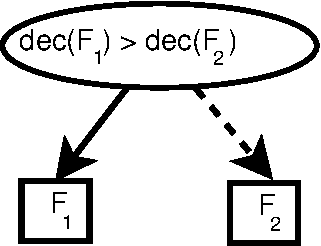
\includegraphics[width=0.1\textwidth]{pics/max_result.pdf}\\
	 \hline
16&          $\min (F_1, F_2)$ &\hspace{3mm}  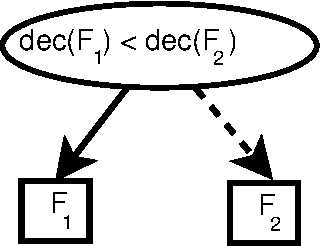
\includegraphics[width=0.1\textwidth]{pics/min_result.pdf}\\
	 \hline
17&	  other& $\mathit{null}$\\
         \hline
    \end{tabular}
  \caption{Input case and result for the method \emph{ComputeResult}
  for binary operations  $\oplus$,  $\ominus$ and $\otimes$ for XADDs.
  %\footnote{Note that for lines 9--12 the zero case should be tested first.}
  }
  \label{tab:ComputeResultXADD}
\end{center}
\end{table}
The other operation required for CA-HMDPs is a continuous maximization over continuous action parameters. As we see in the next section this maximization can be performed symbolically but often produces non-linear inequalities at the decision nodes. This does not effect our symbolic solution theoretically but in practice to prune the resulting XADD using an LP-solver, we require linear decisions. 

The linearize algorithm (in Algorithm~\ref{algLinearize}) is of a recursive nature similar to other XADD algorithms with a \emph{LinearCache} to avoid linearizing the same node. For each node in the XADD starting at the root node, the algorithm linearizes the decision node using \emph{GetRoots} to find the roots of the non-linear function. The algorithm then returns the linear decision nodes. By iterating on the low and high branches of the decision node, all nodes of $F$ are traversed.
%%%%%%%%%%%%%%%%%%%%%%%%%%%%%%%%%%%%%%%%%%%%%%%%%%%%%%%%%%%%%%%%%%%%%%%%%%
%\vspace{10mm}
%\begin{figure}[t!]
%%\centering
%%\subfigure{
%\hspace{-20mm}
%\vspace{-15mm}
%\includegraphics[width=1.27\textwidth]{Figures1/diagrams/reorder.pdf}
%\vspace{-40mm}
%
%\caption{\footnotesize reordering substitute and max.}
%\vspace{-8mm}
%\end{figure}
%%%%%%%%%%%%%%%%%%%%%%%%%%%%%%%%%%%%%%%%%%%%%%%%%%%%%%%%%%%%%%%%%%%%%%%%%%

\subsubsection{Binary XADD Operations}

For \emph{all} binary operations, the function \emph{Apply}($F_1,F_2,\mathit{op}$) (Algorithm \ref{algApply}) computes the resulting XADD. 
%Table \ref{tab:ComputeResultXADD} which is implemented as a function \emph{ComputeResult} defines the result of XADD operations in special cases to avoid unnecessary computation in \emph{Apply}.
%Any operation with two XADDs, $F_1$ and $F_2$, results in a new canonical XADD $F_r$, with eventually a new root node $F^{var}_r$ and two new sub-diagrams $F_h$ and $F_l$.
Two reduced XADD operands $F_1$ and $F_2$ and a binary operator $\mathit{op} \in \{ \oplus, \ominus, \otimes , \max , \min \} $ are the input to the \emph{Apply} algorithm . The output result is a reduced XADD after applying the binary operation. 

Briefly if the result of this algorithm is a quick computation of Table \emph{ComputeResultXADD} it can be immediately returned. Otherwise it checks the \emph{ApplyCache} for any previously stored apply result.  If there is not a cache hit, the earliest decision in the ordering to branch is chosen according to Algorithm~\ref{algChooseDecBranch}. Two recursive \emph{Apply} calls are then made on the branches of this decision to compute $F_l$ and $F_h$. Finally \emph{GetNode} checks for any redundancy before storing it in the cache and returning the resulting XADD. 

Specifically this algorithm can be described using the following steps:

%%%%%%%%%%%%%%%%%%%%%%%%%%%%%%%%%%%%%%%%%%%%%%%%%%%%%%%%%%%%%%%%%
\incmargin{0.5em}
\linesnumbered
\begin{algorithm}[t!]
\SetKwFunction{computeResult}{{\sc ComputeResult}}
\SetKwFunction{Reorder}{{\sc Reorder}}
\SetKwFunction{apply}{Apply} \SetKwFunction{getNode}{{\sc GetNode}}
\SetKwFunction{chooseEarliestDec}{{\sc ChooseEarliestDec}}
\SetKwInOut{Input}{input} \SetKwInOut{Output}{output}
\dontprintsemicolon
%\Input{$F_1$ (root node id for operand 1),\\
%$F_2$ (root node id for operand 2),\\
%$\mathit{op}$ (binary operator, $\mathit{op} \in \{
%\oplus, \ominus, \otimes \}$)}
%\Output{$F_r$ (root node id for the resulting reduced XADD)}
\Begin{
   //check if the result can be immediately computed\\
   \If{\computeResult{$F_1,F_2,\mathit{op}$} $\rightarrow F_r \neq \mathit{null}$}
      {
      \Return{$F_r$}\;
      }
   //check if we previously computed the same operation\\
   \If{$\langle F_1,F_2,\mathit{op}\rangle \rightarrow F_r$ is not in \emph{ApplyCache}}
   {
      //choose decision to branch\\
      $\mathit{dec} =$ \chooseEarliestDec{$F_1,F_2$}\; 
   //set up nodes for recursion\\
   \eIf{$F_1$ is non-terminal $\wedge\ \mathit{dec}=\mathit{dec}_1$}
   {
    $F_l^{v1}=F_{1,l}$\;
    $F_h^{v1}=F_{1,h}$\; 
   }
   {
     $F_{l,h}^{v1}=F_{1}$\;
   }
   \eIf{$F_2$ is non-terminal $\wedge\ \mathit{dec}=\mathit{dec}_2$}
   {
     $F_l^{v2}=F_{2,l}$\;
     $F_h^{v2}=F_{2,h}$\; 
   }
   {
     $F_{l,h}^{v2}=F_{2}$\;
   }
   //use recursion to compute true and false branches for resulting XADD\\
   $F_l=$ \apply{$F_l^{v1},F_l^{v2},\mathit{op}$}\;    
   $F_h=$ \apply{$F_h^{v1},F_h^{v2},\mathit{op}$}\; 
   $F_r=$ \getNode{$\mathit{dec},F_h,F_l$}\;
    //Use Algorithm~\ref{alg:reorder} to reorder decisions\\
   $F_r=$ \Reorder{$F_r$}\;
   //save the result to reuse in the future\\
   insert $\langle F_1,F_2,\mathit{op}\rangle \rightarrow F_r$ into ApplyCache\;
   }
   \Return{$F_r$}\;
}
\caption{{\sc Apply}($F_1,F_2,\mathit{op}$) $\longrightarrow$ $\langle F_r \rangle$ \label{algApply}}
\end{algorithm}
\decmargin{0.5em}
%%%%%%%%%%%%%%%%%%%%%%%%%%%%%%%%%%%%%%%%%%%%%%%%%%%%%%%%%%%%%%%%%

\textbf{Terminal computation}: 
The function \emph{ComputeResult} in line 3 determines if the result of a computation can be immediately computed without recursion. The entries denote a number of pruning optimizations that immediately return a node without recursion. For the discrete maximization (minimization) operation (entries 11--16) , for every two leaf nodes $f$ and $g$ an additional decision node $f > g$ ($f < g$) is introduced to represent the maximum(minimum). This may cause out-of-order decisions reordered by Algorithm~\ref{alg:reorder}. 

\textbf{Caching}:
If the result of 	\emph{ComputeResult} is empty, in the next step we check the \emph{ApplyCache} of line 6 for any previously computed operation using this set of operands and operations. To increase the chance of a match, all items stored in a cache are reduced XADDs.

\textbf{Recursive computation}:
If a call to Apply is unable to immediately compute a result or reuse a previously cached computation, we must recursively compute the result. If both operands are constant terminal nodes the function \emph{ComputeResult} takes care of the result and for the rest of the cases one of the following conditions applies: 
\begin{itemize}
\item $F_1$ or $F_2$ is a constant terminal node or $\mathit{dec}_1\neq \mathit{dec}_2 $: The high and low branch of the operand chosen by \emph{ChooseEarliestDec} (here $F_2$) is applied with the other operand $F_1$. The result of these two \emph{Apply} functions are used with the constraint decision node of $\mathit{dec}_2$ for a reduced result:
\begin{align*}
F_h &= Apply (F_1 , F_{2,h},op) \\
F_l &= Apply (F_1 , F_{2,l},op)  \\
F_r &= GetNode (\mathit{dec}_2 , F_h,F_l) 
\end{align*}
\item $F_1$ and $F_2$ are constant nodes and $\mathit{dec}_1=\mathit{dec}_2 $: Since the decision constraints are equal, the final result is a decision with the constraint of $\mathit{dec}_1 (=\mathit{dec}_2)$ and the high branch is calling \emph{Apply} on the high branches of $F_1$ and $F_2$ and the low branch is defined as the result of the \emph{Apply} function on the low branches:
\begin{align*}
F_h &= Apply (F_{1,h} , F_{2,h},op)  \\
F_l &= Apply (F_{1,l} , F_{2,l},op)  \\
F_r &= GetNode (\mathit{dec}_1 , F_h,F_l) 
\end{align*}
\end{itemize}
Finally for the high and low branch of the final computation, two recursive calls are made to \emph{Apply} and the result is a reduced XADD returned by \emph{GetNode} where the decisions are ordered by \emph{Reorder}. 

\subsection{XADD representation for continuous maximization}

The operation of continuous maximization can also be defined in this structure.
Each XADD path from root to
leaf node is treated as a single case partition with conjunctive constraints.  
$\max_y$ is performed at each leaf subject to these constraints
and all path $\max_y$'s are then accumulated via the $\casemax$
operation to obtain the final result.

A single step of this algorithm is presented in Figure~\ref{fig:xadd_max}. This example is more complex compared to the CAIC partition mentioned above since it has to consider the function root XADD as well as the upper and lower bounds. The input to this illustrated step is the leaf node obtained after the regression step of Algorithm \ref{alg:regress} and decisions leading to this leaf (high or low branches).  The XADD representation is used to represent all intermediate results and also the final result. 
%%%%%%%%%%%%%%%%%%%%%%%%%%%%%%%%%%%%%%%%%%%%%%%%%%%%%%%%%%%%%%%%%%%%%%%%%%
%\vspace{10mm}
\begin{figure}[t!]
%\centering
%\subfigure{
%\hspace{-20mm}
%\vspace{-15mm}
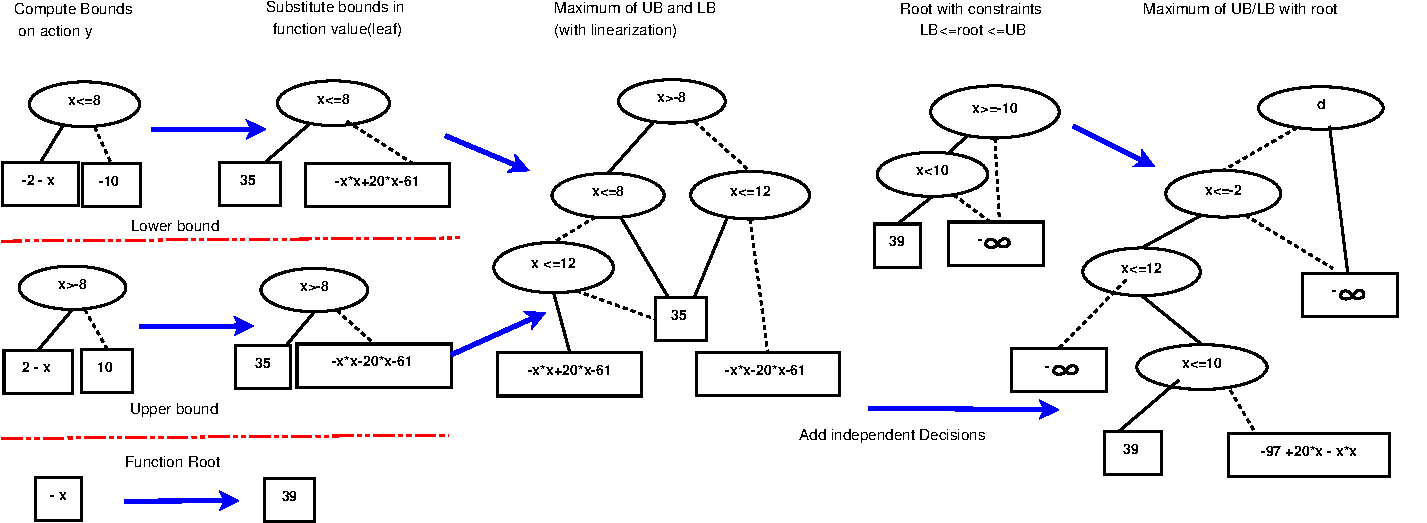
\includegraphics[width=0.97 \textwidth]{pics/maximum_cont_action4.pdf}
%\vspace{-40mm}

\caption{%\footnotesize 
One step of Continuous Maximization algorithm using XADDs for partition:
$\phi_i ( x,d,y ) \equiv \neg d \wedge ( x>2 ) \wedge ( -10 < y < 10) \wedge ( -2 < x+y < 2 )$  
and value $f_i ( x,y ) = 39- y^2 -x^2 - 2a \times x$.}
%The upper and lower bounds of action $y$ and the root is represented by XADDs and substituted inside the leaf node. The maximum of the upper and lower bound is then represented after linearizing the result. The final result takes the maximum of this and the root considering the constraints and independent decisions.}
\label{fig:xadd_max}
\end{figure}
%%%%%%%%%%%%%%%%%%%%%%%%%%%%%%%%%%%%%%%%%%%%%%%%%%%%%%%%%%%%%%%%%%%%%%%%%%

Having defined the efficient representation of XADDs, next we show results from implementing the SVI algorithms using this structure.

\section{Experimental Results} \label{results}

We implemented two versions of our proposed SVI algorithms using XADDs
--- one with the discrete setting and one with the continuous setting. 
% we compare that does not prune nodes of the XADD and another that uses a linear programming solver to prune unreachable nodes (for problems with linear XADDs) and then performs a satisfiability check to prune redundant paths  --- and tested these algorithms on different problems.

For CA-HMDPs we evaluated SVI on a didactic nonlinear
\MarsRover\ example and two problems from Operations Research (OR) \InventoryControl\ defined in the introduction and \WaterReservoir  all of which are described below. For comparison purposes the DA-HMDPs example domains are discretized by their action space. \footnote{All Java source code and a human/machine readable file format for all domains needed to reproduce
the results in this paper can be found online at
\texttt{http://code.google.com/p/xadd-inference}.}

\subsection{Domains}

\paragraph{\InventoryControl}
The inventory problem mentioned in the introduction is revisited to compare 1-item, 2-item and 3-item inventories for both deterministic and stochastic customer demands. 
\paragraph{\MarsRover}
A \MarsRover state consists of its continuous position $x$ along a given route.  In a given time step, the rover may move a continuous distance $y \in [-10,10]$.  The rover receives its greatest reward for taking a picture at $x=0$, which quadratically decreases to zero at the boundaries of the range $x \in [-2,2]$.  The rover will
automatically take a picture when it starts a time step within the range $x \in [-2,2]$ and it only receives this reward once.

Using boolean variable $b \in \{0,1\}$ to indicate if the picture has
already been taken ($b=1$), $x'$ and $b'$ to denote 
post-action state, and $R$ to denote reward, we 
express the \MarsRover\ CA-HMDP using piecewise dynamics and reward:
%\vspace{-4mm}
\begin{align*} 
\hspace{-2.8mm} P(b'\sq=\sq1|x,b) & = 
\begin{cases}
b \lor (x \geq -2 \land x \leq 2): & \sqm 1.0\\
\neg b \land (x < -2 \lor x > 2):  & \sqm 0.0
\end{cases}  \\
\hspace{-2.8mm} P(x'|x,y) & = \delta \left( x' - \begin{cases}
y \geq -10 \land y \leq 10 : & \hspace{-2mm} x + y \\
y < -10 \lor y > 10 : & \hspace{-2mm} x
\end{cases}
\right)  \\
\hspace{-2.8mm} R(x,b) & = \begin{cases}
\neg b \land x \geq -2 \land x \leq 2 : & 4 - x^2 \\
b \lor x < -2 \lor x > 2 : & 0
\end{cases} 
\end{align*}
%%%%%%%%%%%%%%%%%%%%%%%%%%%%%%%%%%%%%%%%%%%%%%%%%%%%%%%%%%%%%%%%%%%%%%%%%%
\begin{figure}[t!]
%\centering
\begin{minipage}[b]{0.48\linewidth}
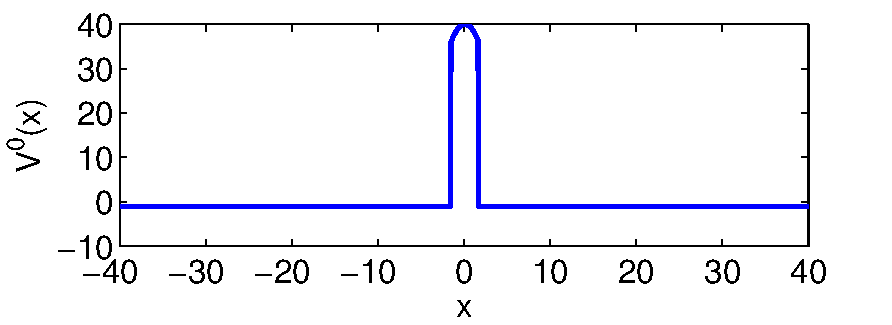
\includegraphics[width=0.9\textwidth]{pics/v1_2d.pdf}\\
%\vspace{-2mm}
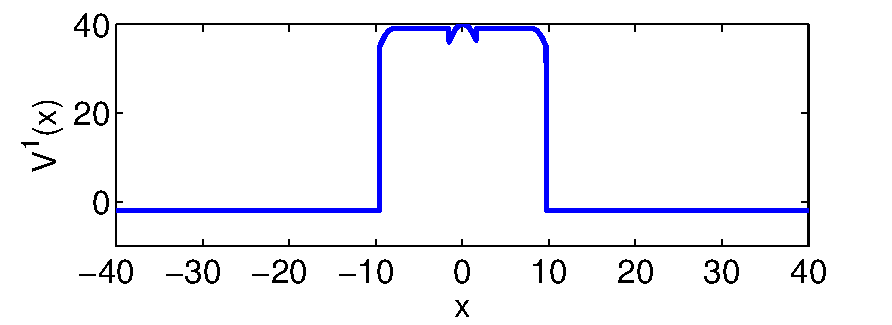
\includegraphics[width=0.9\textwidth]{pics/v2_2d.pdf}\\
%\vspace{-2mm}
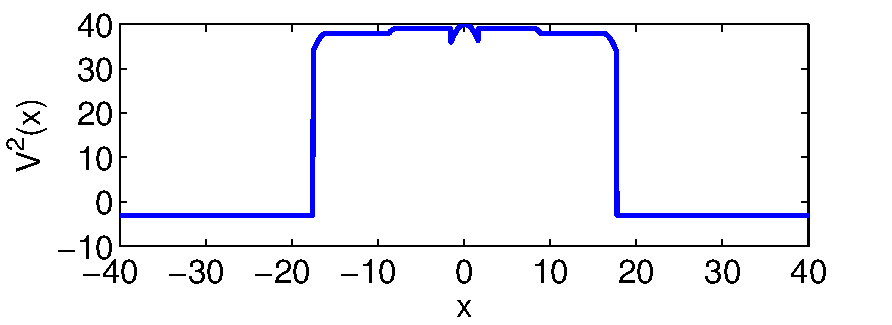
\includegraphics[width=0.9\textwidth]{pics/v3_2d.pdf}
%\vspace{-3mm}

%\parbox{2.8in}{
\caption{\footnotesize Optimal sum of rewards (value) 
$V^t(x)$ for $b = 0 \, 
(\false)$ for time horizons (i.e., decision stages remaining) $t=0$,
$t=1$, and $t=2$ on the \textsc{Continuous Action}  \MarsRover\ problem.  For $x \in [-2,2]$, the
rover automatically takes a picture and receives a reward quadratic in
$x$.  We initialized $V^0(x,b) = R(x,b)$; for $V^1(x)$, the rover achieves
non-zero value up to $x = \pm 12$ and for 
$V^2(x)$, up to $x = \pm 22$.}
\label{fig:opt_graph}

\end{minipage}
%\end{figure}
%%%%%%%%%%%%%%%%%%%%%%%%%%%%%%%%%%%%%%%%%%%%%%%%%%%%%%%%%%%%%%%%%%%%%%%%%%
%%%%%%%%%%%%%%%%%%%%%%%%%%%%%%%%%%%%%%%%%%%%%%%%%%%%%%%%%%%%%%%%%%%%%%%%%%
%\begin{figure}[t!]
%\centering
%\subfigure{
%\hspace{-1mm}
\begin{minipage}[b]{0.48\linewidth}
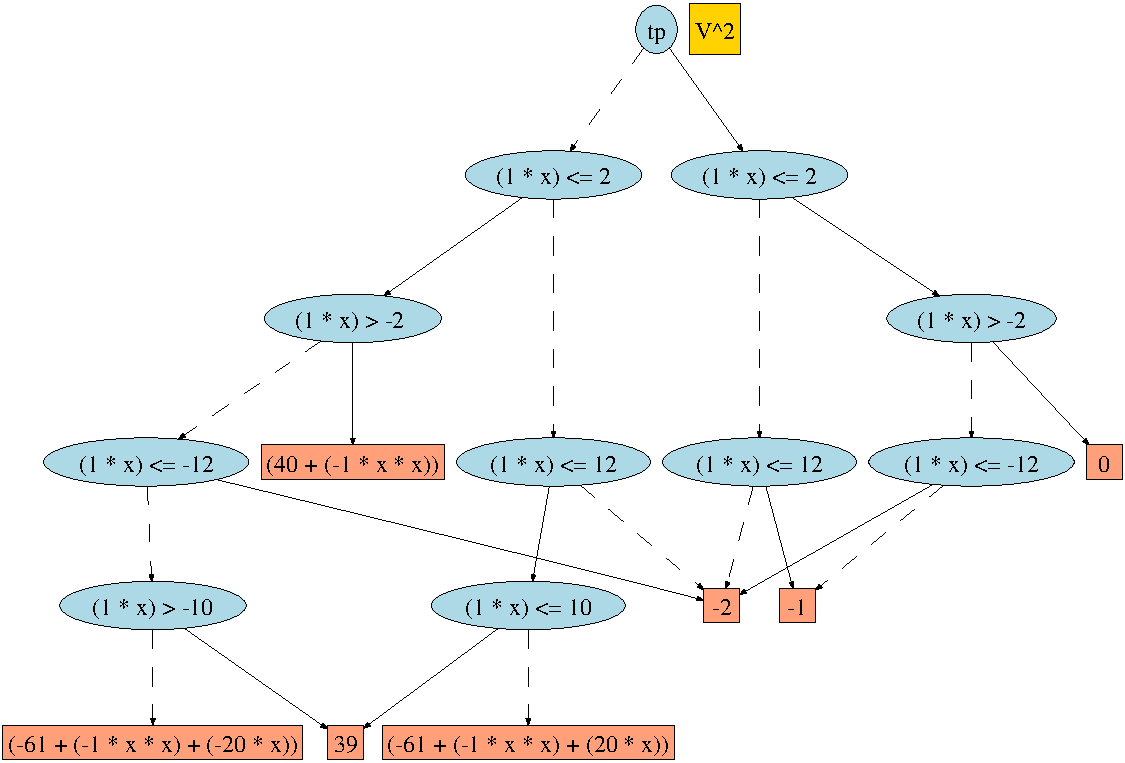
\includegraphics[width=1\textwidth]{pics/roverdot.pdf}
\vspace{6mm}

\caption{\footnotesize Optimal value function $V^2(x)$ for the
\textsc{Continuous Action}  \MarsRover\ problem represented as an (XADD) equal to the second diagram on the left. 
To evaluate
$V^2(x)$ for any state $x$, one simply traverses the diagram in a
decision-tree like fashion until a leaf is reached where the
non-parenthetical expression provides the \emph{optimal value} and the
parenthetical expression provides the \emph{optimal policy} 
($y = \pi^{*,2}(x)$) to achieve value $V^2(x)$.}
\label{fig:opt_val_pol}
\vspace{-5mm}
\end{minipage}
%\vspace{-5mm}
\end{figure}
%%%%%%%%%%%%%%%%%%%%%%%%%%%%%%%%%%%%%%%%%%%%%%%%%%%%%%%%%%%%%%%%%%%%%%%%%%
The maximum long-term \emph{value} $V$ from a given state in \MarsRover\ 
is defined as a function of state variables:
{\footnotesize
%\begin{tabular}{l}
%$
\begin{align*}
V = \begin{cases}
\neg \mathit{take\-pic}_1 \land \mathit{take\-pic}_2 \land (4 -x^2 -y^2\geq 0) \land 
(5 - x^2 - y^2\geq 0) : & 4 -x^2 -y^2 \\
\mathit{take\-pic}_1 \land \neg \mathit{take\-pic}_2 \land (2 -x^2 -y^2\geq 0) \land 
(3 - x^2 - y^2\geq 0) : & 2 -x^2 -y^2 \\
\neg \mathit{take\-pic}_1 \land \mathit{take\-pic}_2 \land (4 -x^2 -y^2\geq 0) \land 
(5 - x^2 - y^2\leq 0) : & -1 \\
\mathit{take\-pic}_1 \land \neg \mathit{take\-pic}_2 \land (2 -x^2 -y^2\geq 0) \land 
(3 - x^2 - y^2\leq 0) : & -1 \\
else &: 0 \\
\end{cases} 
%$
%\end{tabular}
\end{align*}
}
The value function is piecewise and non-linear, and contains non-rectangular decision
boundaries like $4 -x^2 -y^2\geq 0$. Figure~\ref{fig:opt_val_pol} presents the  0-, 1-, and 2-step time horizon solution for this problem. Despite the intuitive and simple nature of this result, we are unaware of prior methods that can produce such exact solutions. 

\paragraph{\WaterReservoir} 
Reservoir management is well-studied in
the OR literature \cite{Mahootchi2009,Yeh1985}.  The key continuous decision is how
much elapsed time $e$ to
\emph{drain} (or \emph{not drain}) each reservoir to maximize
electricity revenue over the decision-stage horizon while avoiding
reservoir overflow and underflow.  Cast as a CA-HMDP, we 
believe SVI provides the first approach capable of deriving
an exact closed-form non-myopic optimal policy
for all levels.

We examine a 2-reservoir problem with
respective levels $(l_1,l_2)\in [0,\infty]^2$ with reward penalties for 
overflow and underflow and a reward gain linear in the elapsed time $e$ for
electricity generated in periods when the $\mathit{drain}(e)$ action
drains water from $l_2$ to $l_1$ (the other action is 
$\mathit{no}$-$\mathit{drain}(e)$); we assume deterministic rainfall
replenishment and present the reward function as:  

\vspace{-4mm}
{\footnotesize
\begin{align*}
R & = \begin{cases}
((50-200*e) \leq l_1 \leq (4500-200*e)) \wedge ((50+100*e) \leq l_2 \leq (4500+100*e)) %\\ \hspace{4mm} \vspace{3mm} 
&:e\\
((50+300*e) \leq l_1 \leq (4500+300*e)) \wedge ((50-400*e) \leq l_2 \leq (4500-400*e)) %\\ \hspace{4mm} \vspace{3mm} 
&:0\\
\text{\normalsize otherwise} &: -\infty \\
\end{cases}
\end{align*}}
The transition function for levels of the $\mathit{drain}$ action is defined below. Note that for the $\mathit{no}$-$\mathit{drain}$ action, the $\mathit{500 * e}$ term is not involved.
{%\footnotesize 
\begin{align*}
l_1' & =(400 * e + l_1 -700 * e + 500 * e) \\
l_2'& =(400 * e + l_2 - 500 * e) \\
\end{align*}}

Similar to the discrete version of the \InventoryControl problem in the introduction, the DA-HMDP setting for these two problems defines discrete actions by partitioning the action space of each domain into $i$ number of slices. For example the \MarsRover\ problem with 2 actions which are the lower and upper bounds on $a$ ($a_1=-10, a_2 = 10$) and the transition and reward functions are defined according to these constant values.
We now provide the empirical results obtained from implementing our algorithms.

\subsection{Results}

For both the \textsc{Discrete Action} and \textsc{Continuous Action} \MarsRover\ domains, 
we have run experiments to evaluate our SDP solution 
in terms of time and space cost while varying the horizon and problem size.

%%%%%%%%%%%%%%%%%%%%%%%%%%%%%%%%%%%%%%%%%%%%%%%%%%%%%%%%%%%%%%%%%%%%%%%%%%
\begin{figure*}[t]
\centering
%\subfigure{
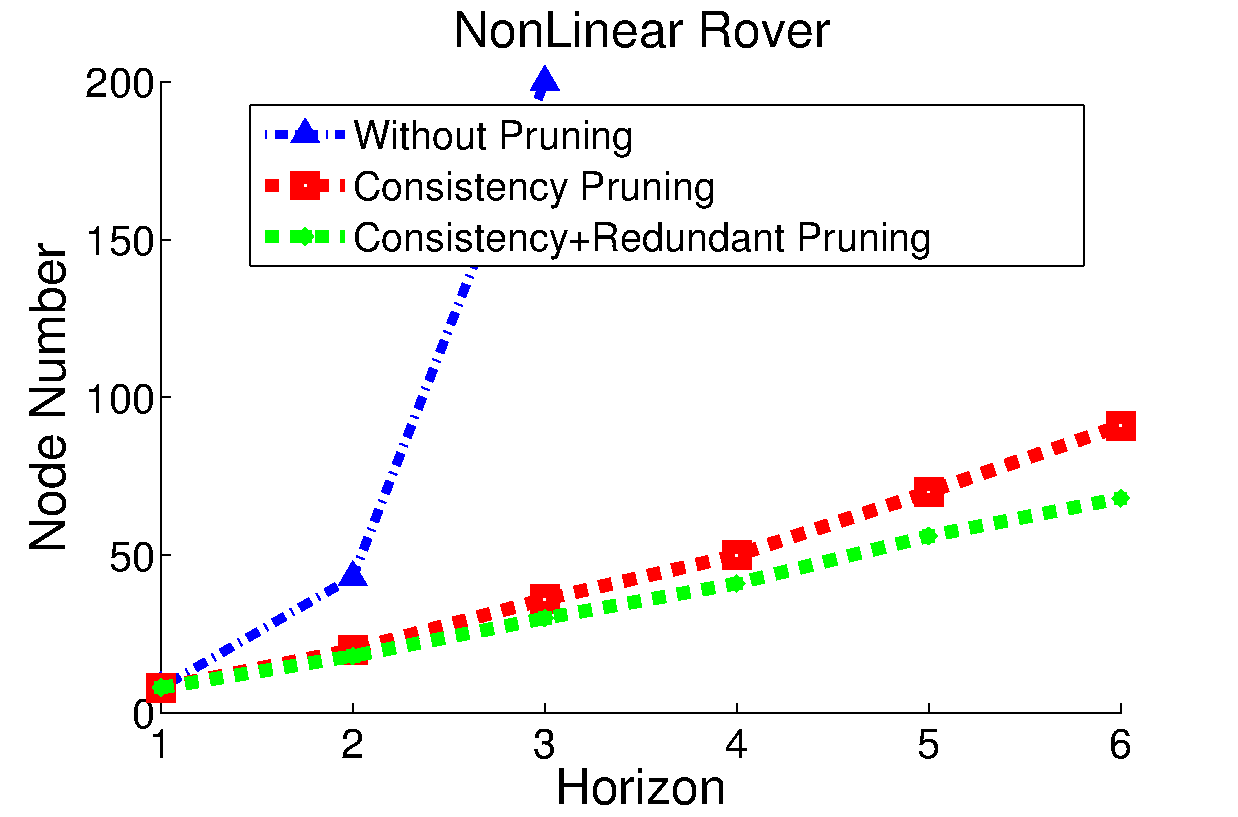
\includegraphics[width=0.45\textwidth]{pics/contRoverNode2.pdf}
%\hspace{5mm}
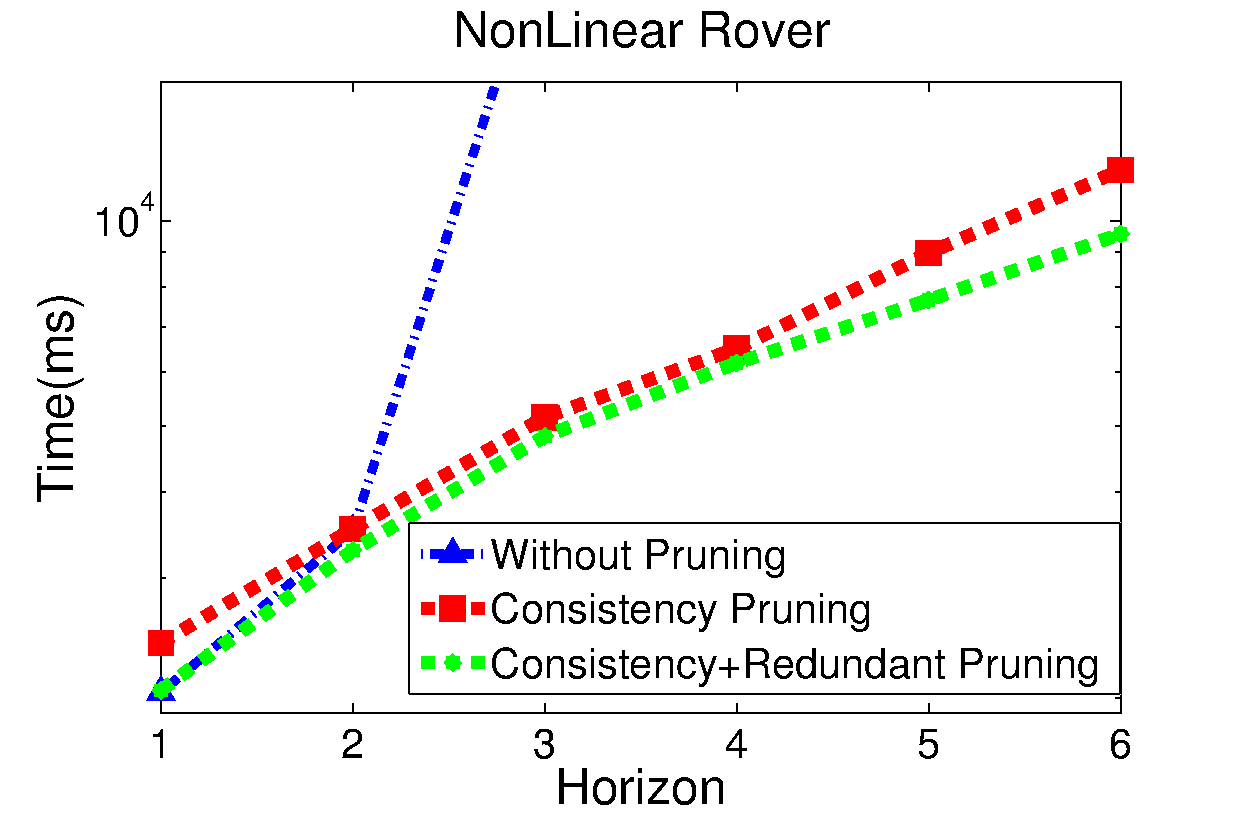
\includegraphics[width=0.45\textwidth]{pics/contRoverTime2.pdf}
%}
\vspace{-3mm}
\caption{%\footnotesize 
Space (\# XADD nodes in value function) and
time for different iterations (horizons) of SDP on Nonlinear \textsc{Continuous Action}  \MarsRover\ with 4 different results based on pruning techniques. Results are shown for  the XADD 
 with no pruning technique, with only consistency checking (using LP-solver) and with both the consistency and redundancy checking with a numerical precision heuristic.} %does it need more explaining? 
\label{fig:roverTS}
\end{figure*}
%%%%%%%%%%%%%%%%%%%%%%%%%%%%%%%%%%%%%%%%%%%%%%%%%%%%%%%%%%%%%%%%%%%%%%%%%%

%%%%%%%%%%%%%%%%%%%%%%%%%%%%%%%%%%%%%%%%%%%%%%%%%%%%%%%%%%%%%%%%%%%%%%%%%%
%figure5 : time-iteration and space-iteraton for 1d-2d-noPrune inventory
\begin{figure}[tbp!]
\vspace{2mm}
\centering
%\subfigure{
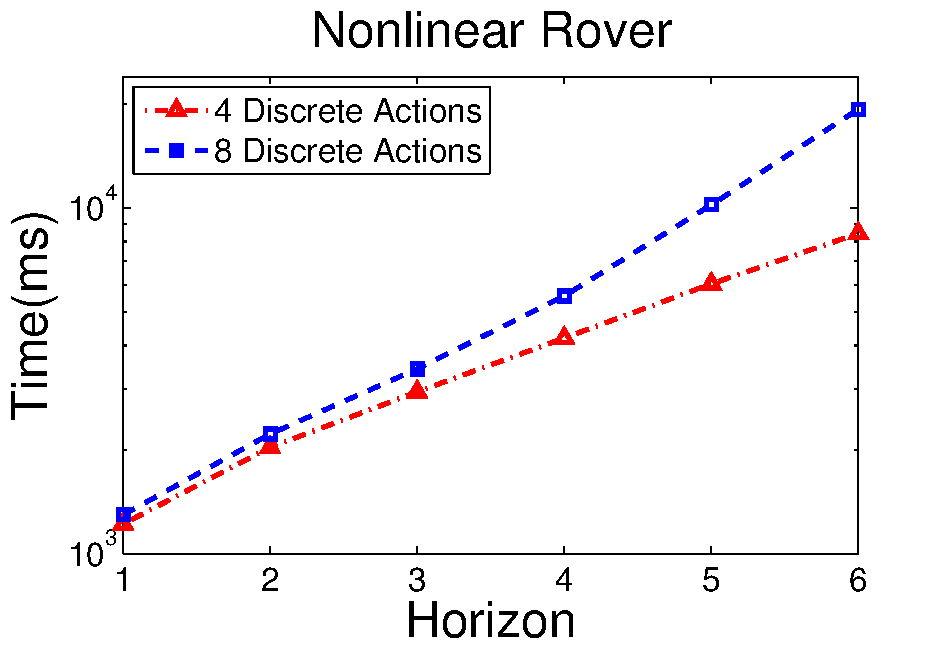
\includegraphics[width=0.45\textwidth]{pics/DisRoverNode.pdf}
\hspace{2mm}
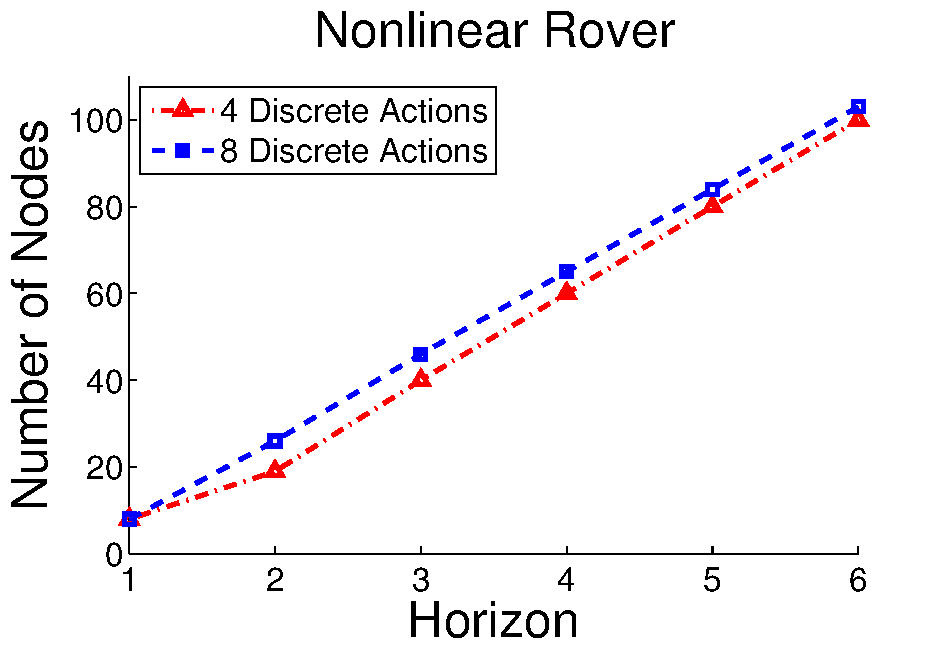
\includegraphics[width=0.45\textwidth]{pics/DisRoverTime.pdf}
%}
\vspace{-2mm}
\caption{%\footnotesize 
Space and elapsed time vs. horizon for a fixed discretization of 4 and 8 for the \MarsRover domain. This demonstrates how the number of nodes and time increases for each horizon. 
}
\label{fig:roverDisTS}
\vspace{-1mm}
\end{figure}
%%%%%%%%%%%%%%%%%%%%%%%%%%%%%%%%%%%%%%%%%%%%%%%%%%%%%%%%%%%%%%%%%%%%%%%%%%

For the \textsc{Continuous Action} \MarsRover problem, we present the time and space analysis in Figure~\ref{fig:roverTS}. Here three evaluations are performed based on the pruning algorithms of Section~\ref{sec:pruningAlg}. We note that without the inconsistency checking of Algorithm~\ref{algPrune}, SDP can not go beyond the third iteration as it produces many inconsistent nodes. The comparison is performed with consistency pruning and redundancy checking. The full pruning experiment also uses a numerical heuristic that omits similar branches. %With the full pruning of Algorithm~\ref{algRedundant} less than 10 \% node reduction is achieved but due to the calls made to the SAT-Solver the time increases to more than 10 times of that of the heuristic pruning. 
However even with the heuristic approach very little node reduction can be gained from redundancy pruning. This suggests that in some domains using redundancy pruning in not efficient and should be omitted from the final results. 
Hence we will present results for the \WaterReservoir and \InventoryControl problem with only consistency pruning. 

Next we present the analysis of the \textsc{Discrete Action} \MarsRover\ domains. Figure~\ref{fig:roverDisTS} shows how time and space costs of different horizons increases for a fixed action discretization of 4 and 8.
Note that one of the caveats of using a discrete setting is defining the actual discrete actions. In the continuous setting an action is defined between a large high and low range (e.g $a \in$ [$-1000000,1000000$]) allowing the SDP algorithm to choose the best possible action among all the answers. However for a discrete setting, choosing the range to discretize the action becomes very important. As an example in the rover description, allowing actions to be far from the center (e.g. $a \in$ [$-20,20$]) does not result in a converged solution. Finding this range is one of the drawbacks of using a discrete setting. 
%%%%%%%%%%%%%%%%%%%%%%%%%%%%%%%%%%%%%%%%%%%%%%%%%%%%%%%%%%%%%%%%%%%%%%%%%%
%figure5 : time-iteration and space-iteraton for 1d-2d-noPrune inventory
\begin{figure}[tbp!]
\vspace{-2mm}
\centering
%\subfigure{
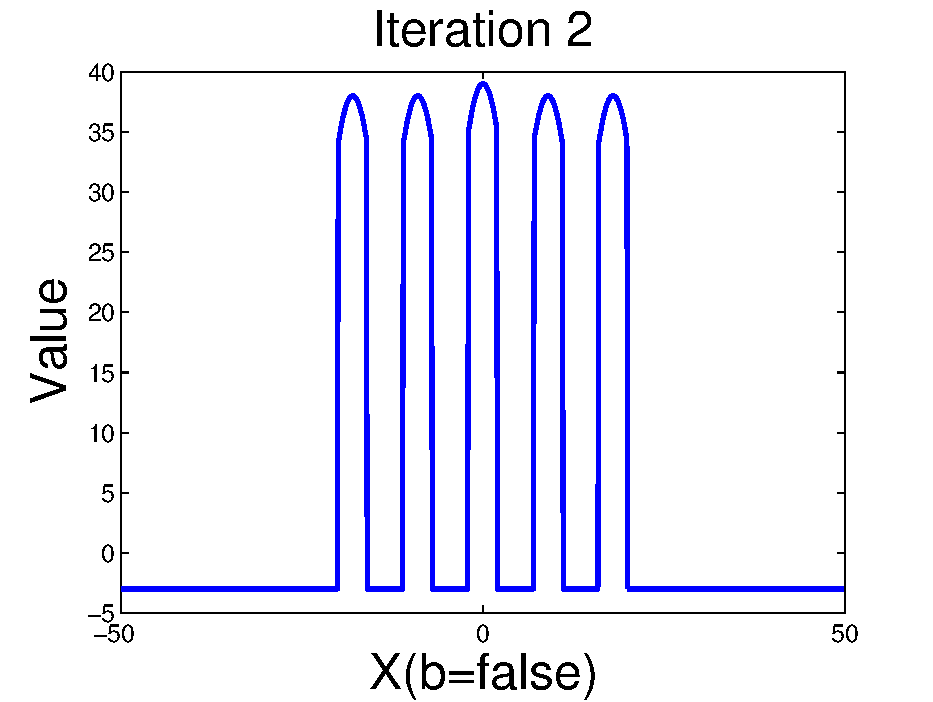
\includegraphics[width=0.18\textwidth]{pics/rover2.pdf}
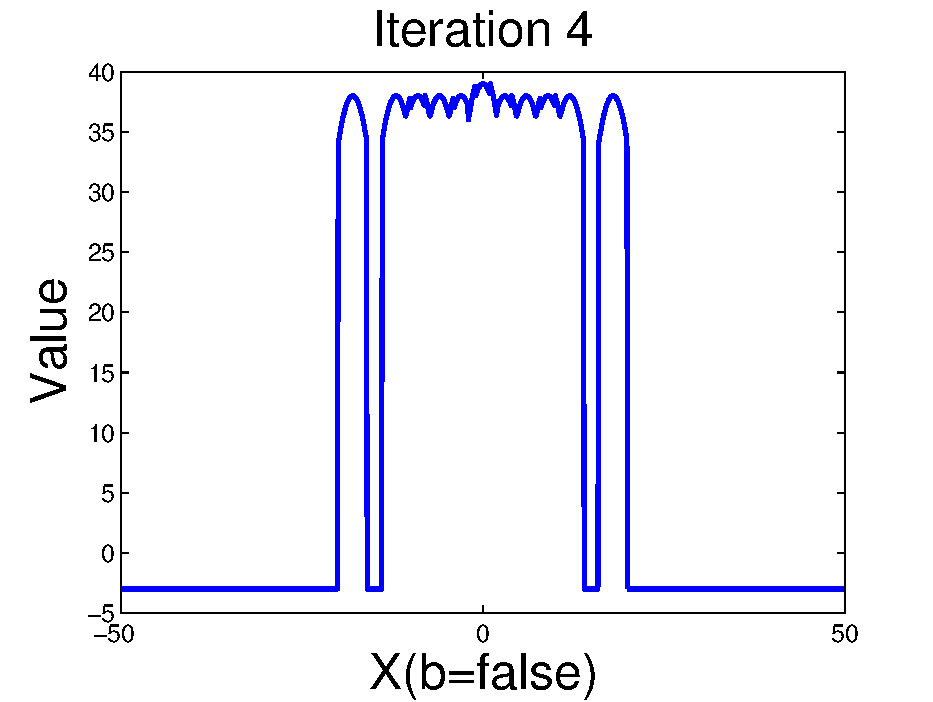
\includegraphics[width=0.18\textwidth]{pics/rover4.pdf}
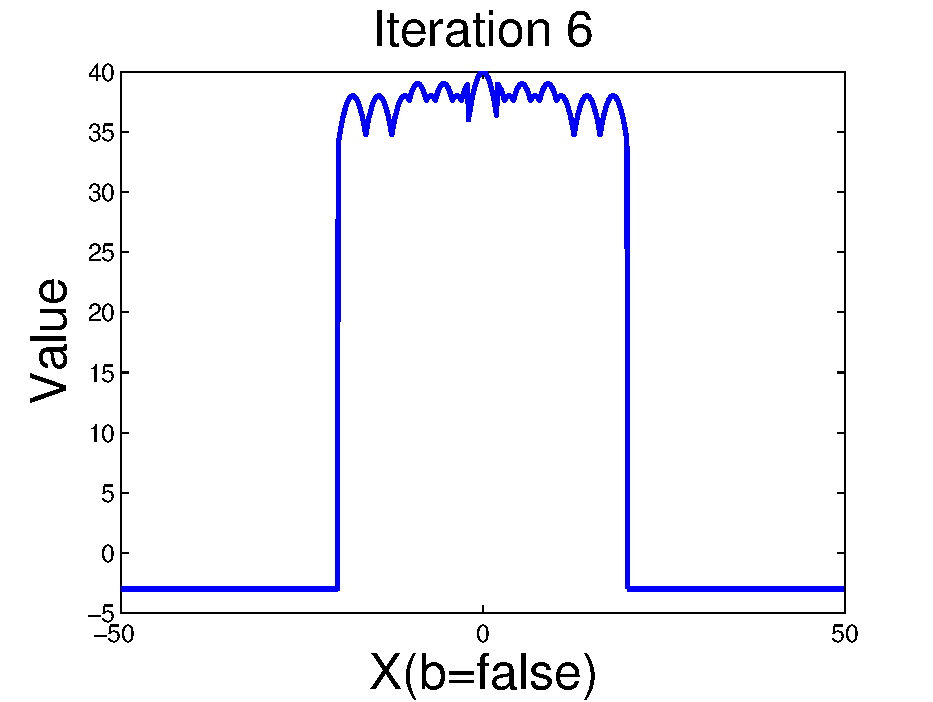
\includegraphics[width=0.18\textwidth]{pics/rover6.pdf}
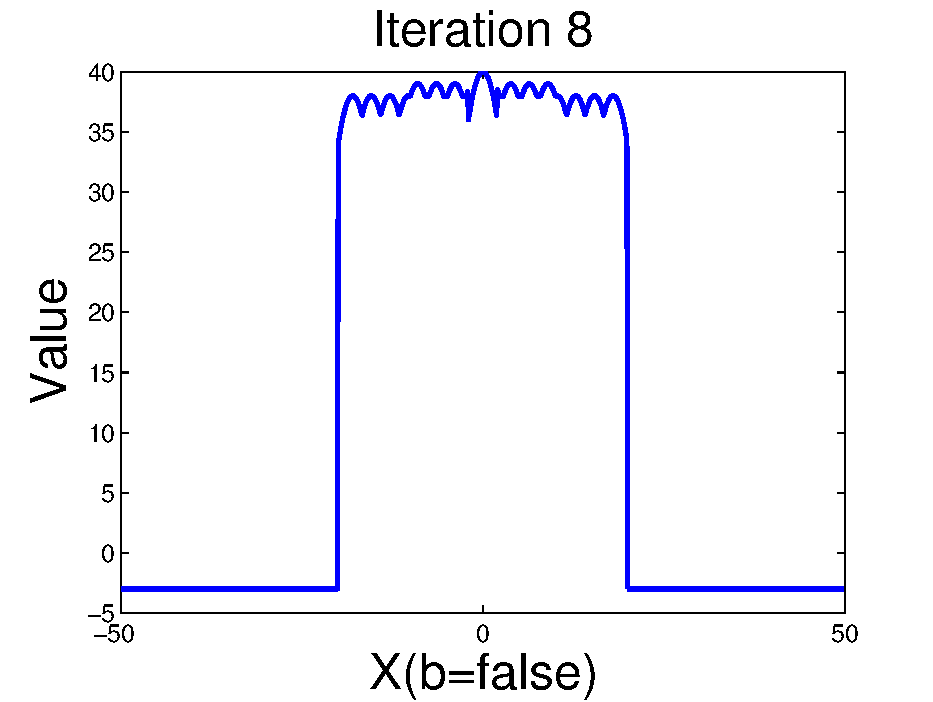
\includegraphics[width=0.18\textwidth]{pics/rover8.pdf}
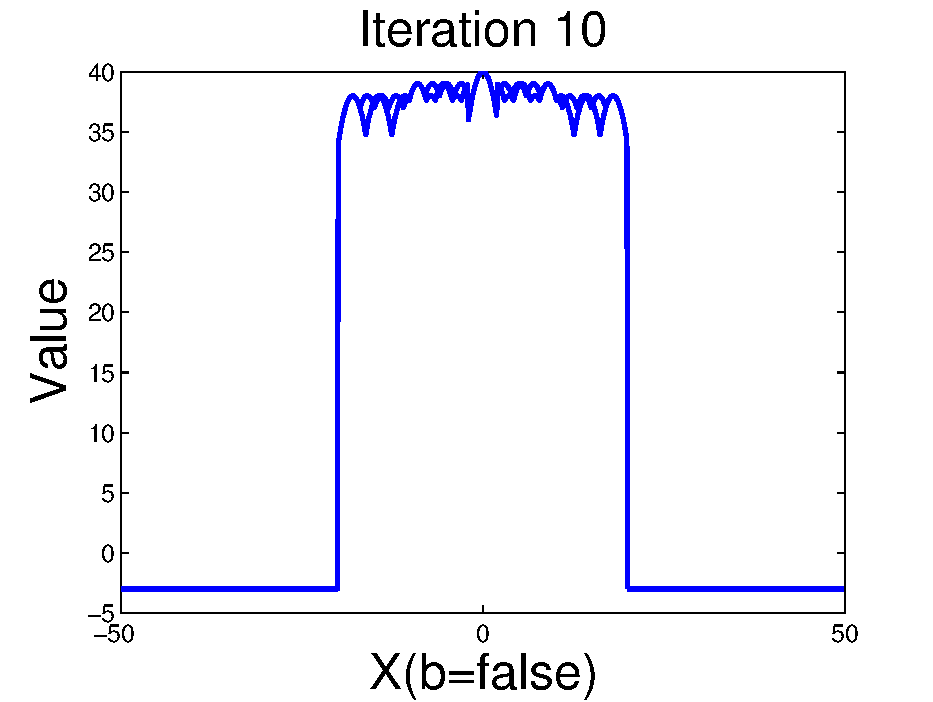
\includegraphics[width=0.18\textwidth]{pics/rover10.pdf}

%}
\vspace{-2mm}
\caption{%\footnotesize 
$V^3$ for different number of \textsc{Discrete Actions} in the \MarsRover\ problem. As the number of discrete actions increases, the value function more closely resembles the continuous action value of $V^3$ (defined in Figure ~\ref{fig:opt_val_pol}).
}
\label{fig:rover_discrete}
\vspace{-1mm}
\end{figure}
%%%%%%%%%%%%%%%%%%%%%%%%%%%%%%%%%%%%%%%%%%%%%%%%%%%%%%%%%%%%%%%%%%%%%%%%%%

On the other hand, the level of discretization within this range is also very important. To show this visually Figure~\ref{fig:rover_discrete} shows the results of the third iteration for 6 different discretizations compared to the continuous result. This figure proves the need to finely partition the action space within the predefined range. However as Figure~\ref{fig:roverDisSize} demonstrates, increasing the number of discrete action (for the fixed horizon of 3), leads to increasing time and space costs. Here results of different level of discretization is similar for the \WaterReservoir problem.

%%%%%%%%%%%%%%%%%%%%%%%%%%%%%%%%%%%%%%%%%%%%%%%%%%%%%%%%%%%%%%%%%%%%%%%%%%
%figure5 : time-iteration and space-iteraton for 1d-2d-noPrune inventory
\begin{figure}[tbp!]
\vspace{-2mm}
\centering
%\subfigure{
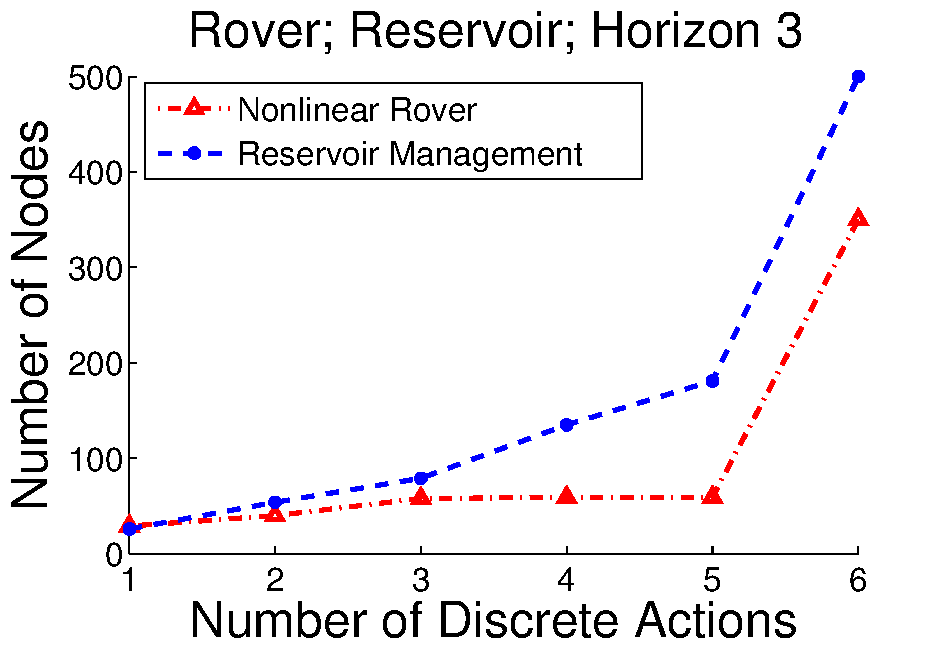
\includegraphics[width=0.45\textwidth]{pics/disRovResNode2.pdf}
\hspace{2mm}
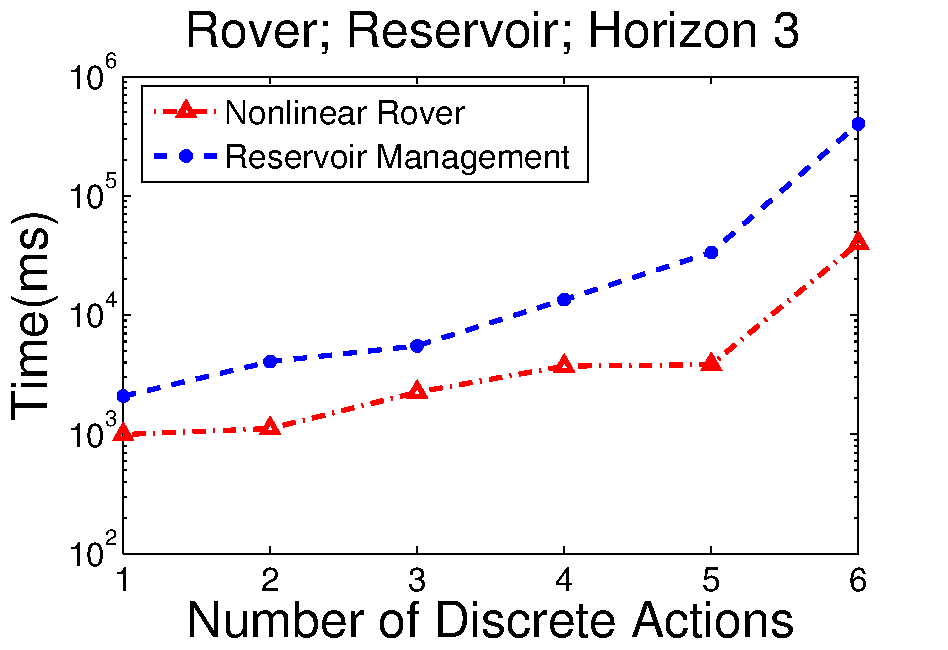
\includegraphics[width=0.45\textwidth]{pics/disRovResTime2.pdf}
%}
\vspace{-2mm}
\caption{%\footnotesize 
Space and elapsed time vs. horizon for a fixed horizon of 3 and different problem sizes for the \textsc{Discrete Action} \MarsRover\ and the \WaterReservoir. 
}
\label{fig:roverDisSize}
\vspace{-5mm}
\end{figure}
%%%%%%%%%%%%%%%%%%%%%%%%%%%%%%%%%%%%%%%%%%%%%%%%%%%%%%%%%%%%%%%%%%%%%%%%%%

%%%%%%%%%%%%%%%%%%%%%%%%%%%%%%%%%%%%%%%%%%%%%%%%%%%%%%%%%%%%%%%%%%%%%%%%%%
%figure5 : time-iteration and space-iteraton for 1d-2d-noPrune inventory
\begin{figure}[tbp!]
\vspace{2mm}
\centering
%\subfigure{
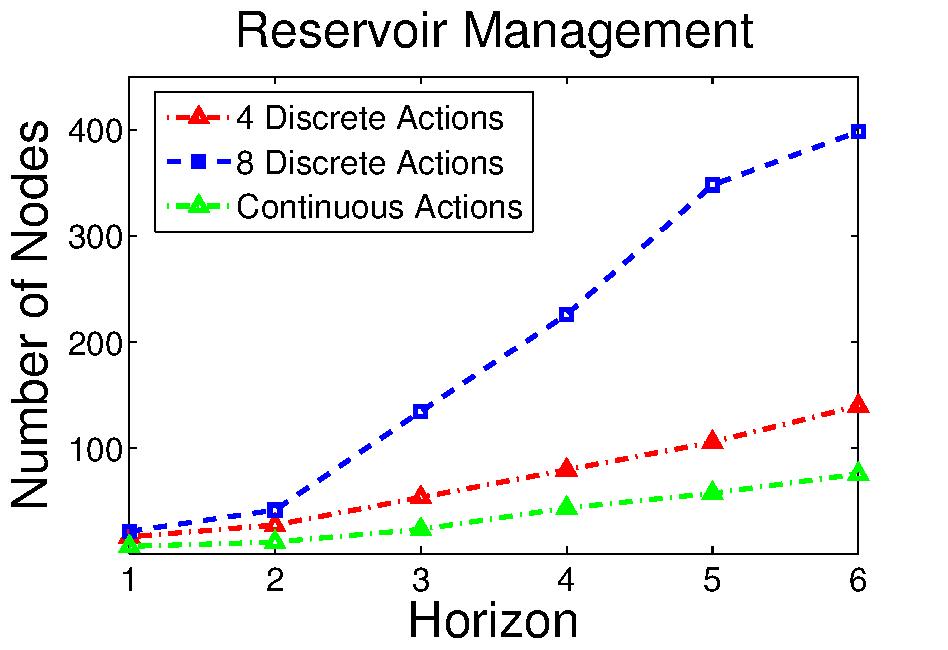
\includegraphics[width=0.45\textwidth]{pics/DisResNode2.pdf}
\hspace{2mm}
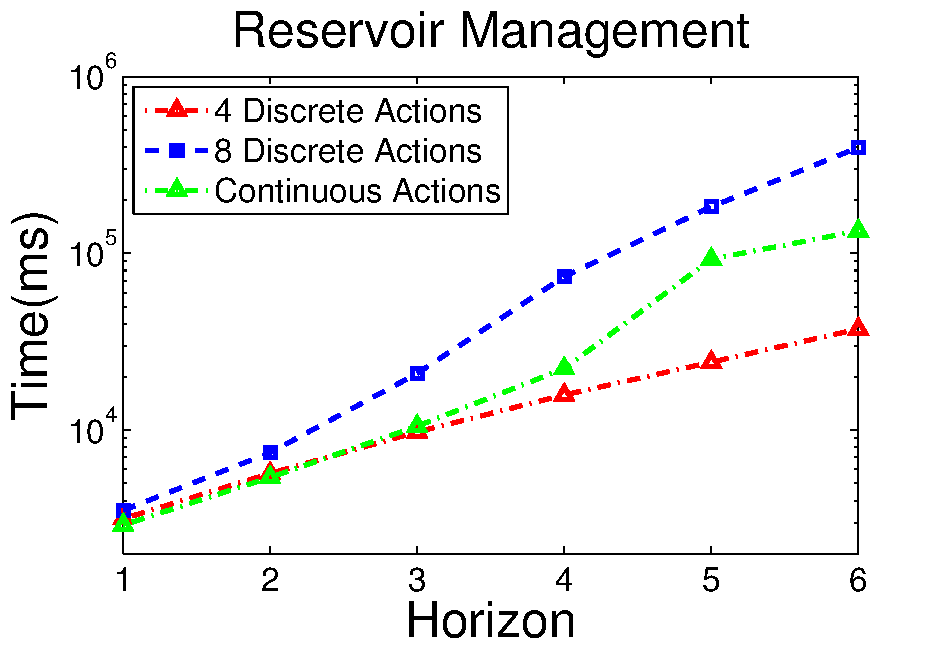
\includegraphics[width=0.45\textwidth]{pics/DisResTime2.pdf}
%}
\vspace{-2mm}
\caption{%\footnotesize 
Space and elapsed time vs. horizon for a fixed discritization of 4 and 8 for the discrete action \WaterReservoir. To compare the time and space of continuous action \WaterReservoir is given. }
\label{fig:resDisTS}
\vspace{-5mm}
\end{figure}
%%%%%%%%%%%%%%%%%%%%%%%%%%%%%%%%%%%%%%%%%%%%%%%%%%%%%%%%%%%%%%%%%%%%%%%%%%

Figure~\ref{fig:resDisTS} presents the time and number of nodes for different horizons for 4 and 8 discrete actions compared to the continuous actions in the \WaterReservoir domain. Although in the first two iterations the time and space of the discrete action setting are similar, however for higher horizons more time and space is required in the 8 discrete action case. The number of nodes are lower for the continuous case compared to both discretizations but the time elapsed is higher than the 4-discrete actions due to the complexity of the continuous action maximization.

%%%%%%%%%%%%%%%%%%%%%%%%%%%%%%%%%%%%%%%%%%%%%%%%%%%%%%%%%%%%%%%%%%%%%%%%%%
\begin{figure*}[tbp!]
%\vspace{-1mm}
\centering
\vspace{10mm}
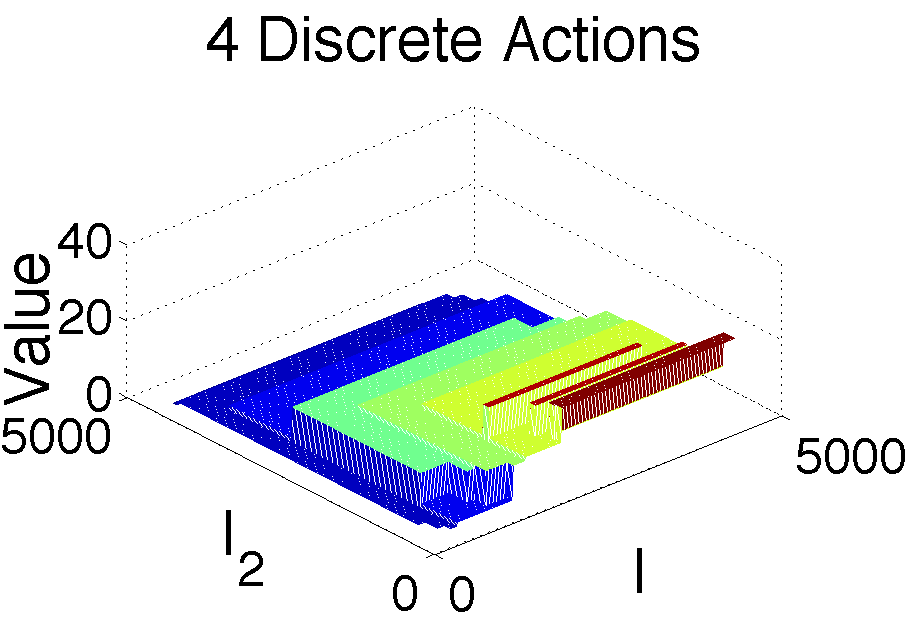
\includegraphics[width=0.48\textwidth]{pics/res3d4.pdf} 
\hspace{2mm}
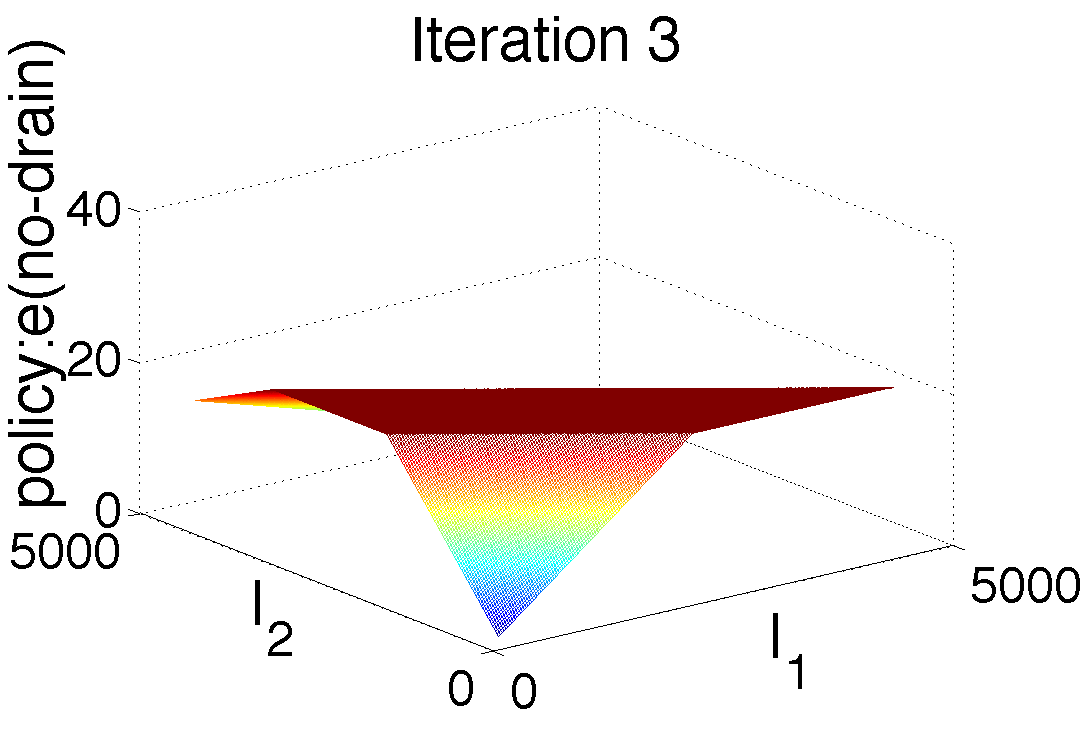
\includegraphics[width=0.48\textwidth]{pics/q3.pdf}
\vspace{10mm}
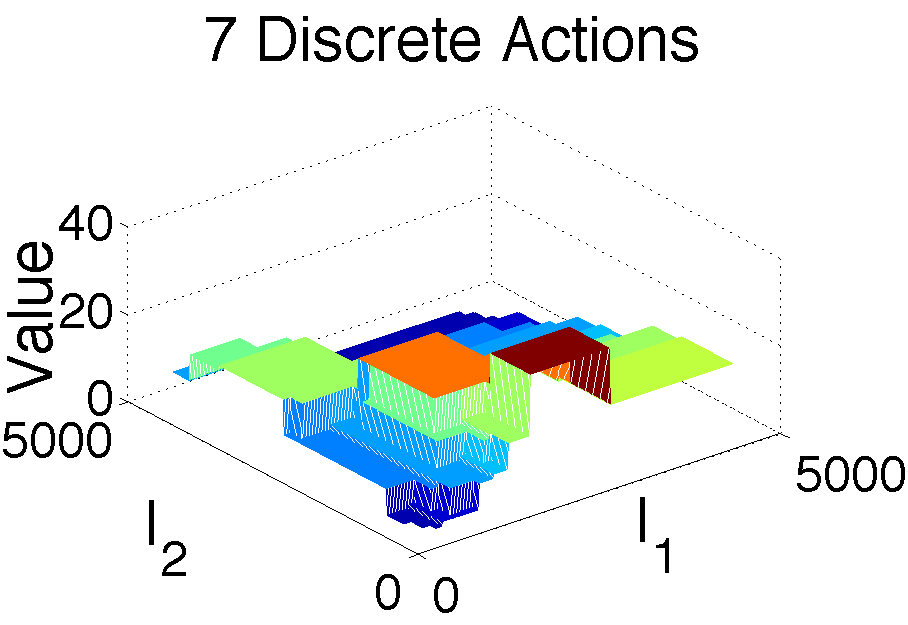
\includegraphics[width=0.48\textwidth]{pics/res3d7.pdf}
\hspace{2mm}
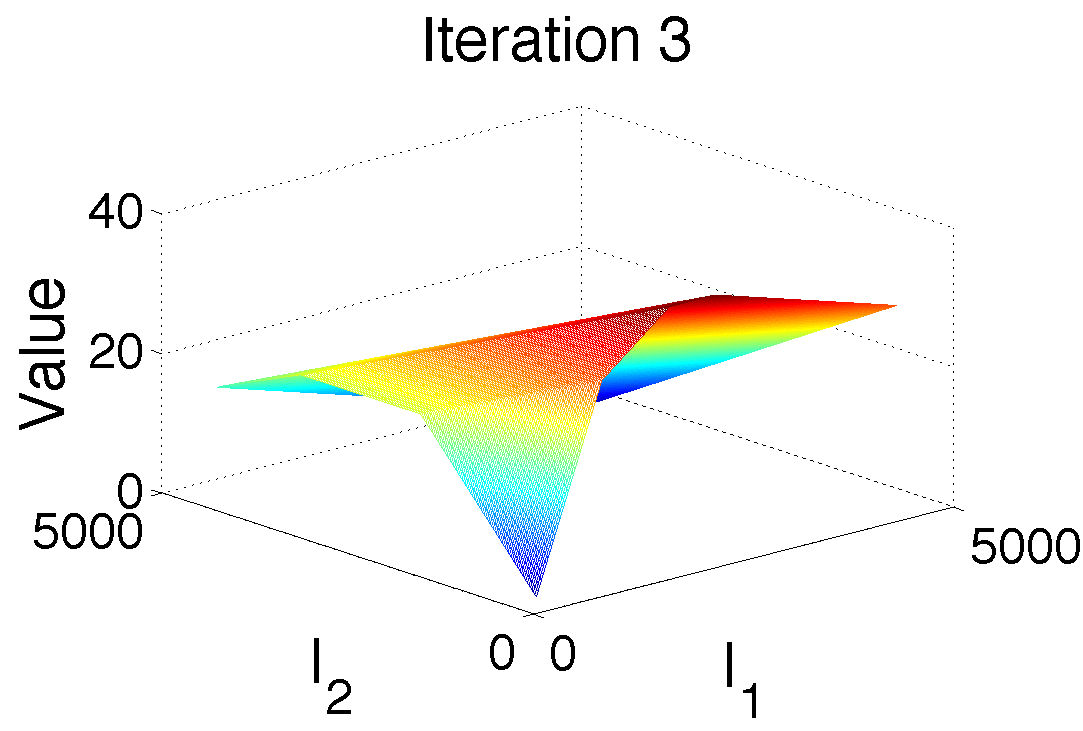
\includegraphics[width=0.48\textwidth]{pics/v3.pdf}
\vspace{10mm}
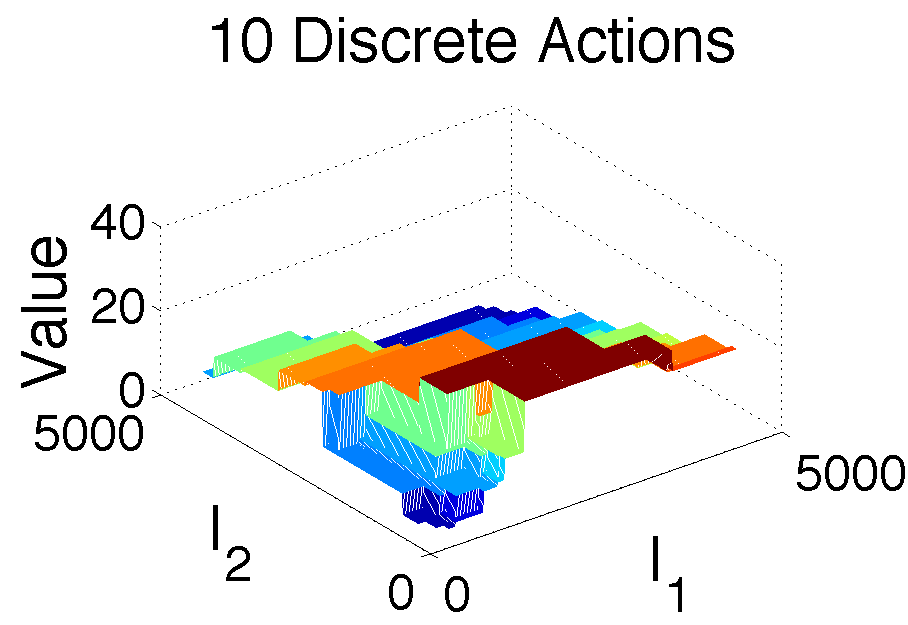
\includegraphics[width=0.48\textwidth]{pics/res3d10.pdf}
\hspace{2mm}
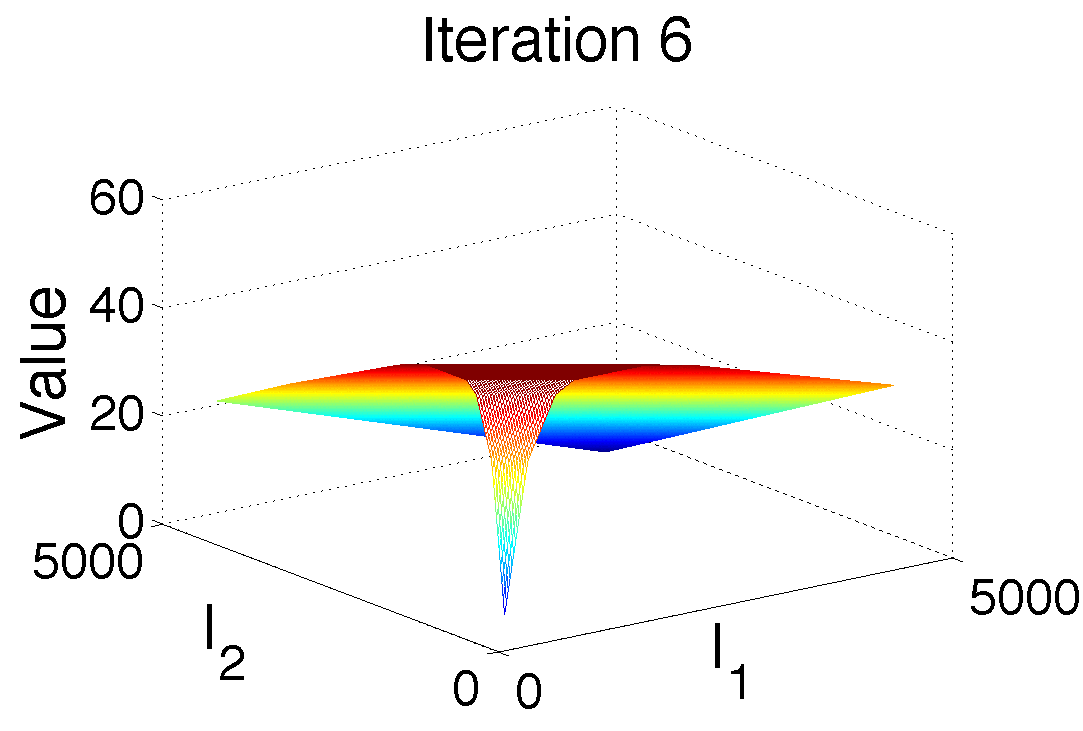
\includegraphics[width=0.48\textwidth]{pics/v6.pdf}
%\vspace{-3mm}
\caption{%\footnotesize 
Results for the \textsc{Discrete Action} and \textsc{Continuous Action} of the \WaterReservoir problem. {\it (left)} 4, 7 and 10 \textsc{Discrete Actions} of the \WaterReservoir problem for different water levels in iteration $V^3$. Each discretization draws the value closer to that of the continuous action \WaterReservoir on the right. {\it (right)} Policy $\mathit{no}$-$\mathit{drain}(e)=\pi^{3,*}(l_1,l_2)$ 
showing on the z-axis the elapsed time $e$ that should be executed 
for $\mathit{no}$-$\mathit{drain}$ conditioned on the states; followed by $V^3(l_1,l_2)$ and $V^6(l_1,l_2)$.
}
\label{fig:discreteplots}
%\vspace{-1mm}
\end{figure*}
%%%%%%%%%%%%%%%%%%%%%%%%%%%%%%%%%%%%%%%%%%%%%%%%%%%%%%%%%%%%%%%%%%%%%%%%%%
Figure~\ref{fig:discreteplots} (left) demonstrates three levels of discretization in the \WaterReservoir problem. The top left figure assumes 4 discrete actions, the middle figure has 7 actions and the bottom figure uses 10 discrete actions. The value of the third iteration is represented for all figures w.r.t. water levels $l_1$ and $l_2$. The figures suggest that finer grain discretization results in better results, closer to that of the continuous action value in middle right figure. 

Furthermore Figure~\ref{fig:discreteplots} (right) plots the  
the optimal closed-form policy at $h=3$: the solution interleaves $\mathit{drain}(e)$ and $\mathit{no}$-$\mathit{drain}(e)$ where even horizons are the latter.
Here we see that we avoid draining for the longest elapsed time $e$ 
when $l_2$ is low (wait for rain to replenish) and $l_1$ is high (draining
water into it could overflow it).  $V^3(l_1,l_2)$ and $V^6(l_1,l_2)$
show the progression of convergence from horizon $h=3$ to $h=6$ ---
low levels of $l_1$ and $l_2$ allow the system to generate electricity
for the longest total elapsed time over 6 decision stages. 

In Figure~\ref{fig:invC}, we provide a time and space analysis of
deterministic- and stochastic-demand (resp. DD and SD) variants of the
SCIC and MJCIC problem for up to three items (the same scale of
problems often studied in the OR literature); for each number of items
$n \in \{ 1,2,3 \}$ the state (inventory levels) is $\vec{x} \in
[0,\infty]^n$ and the action (reorder amounts) is $\vec{y} \in
[0,\infty]^n$.  Orders are made at one month intervals and we solve
for a horizon up to $h=6$ months.  
%Here we see that linear feasibility checking/pruning in the XADD is crucial -- we cannot solve beyond $h=2$ without it for 1 item!  
While solving for larger numbers of
items and SD (rather than DD) both increase time and space, 
the solutions quickly reach quiescence indicating structural
convergence.

Figure~\ref{fig:invD6} represents the time and space for the deterministic \textsc{Discrete Action} \InventoryControl for a discretization of 6 actions and different inventory items for up to $h=6$ horizons. While the number of items affects both time and space, even for 6 discrete actions the 3-item inventory will have exponential time and space for the second horizon onwards. The reason is behind the high dimensions, for a 3-item inventory of 6 discrete actions, a total of $6 \times 6 \times 6$ actions are required!
%%%%%%%%%%%%%%%%%%%%%%%%%%%%%%%%%%%%%%%%%%%%%%%%%%%%%%%%%%%%%%%%%%%%%%%%%%
%figure5 : time-iteration and space-iteraton for 1d-2d-noPrune inventory
\begin{figure}[tbp!]
\vspace{-2mm}
\centering
%\subfigure{
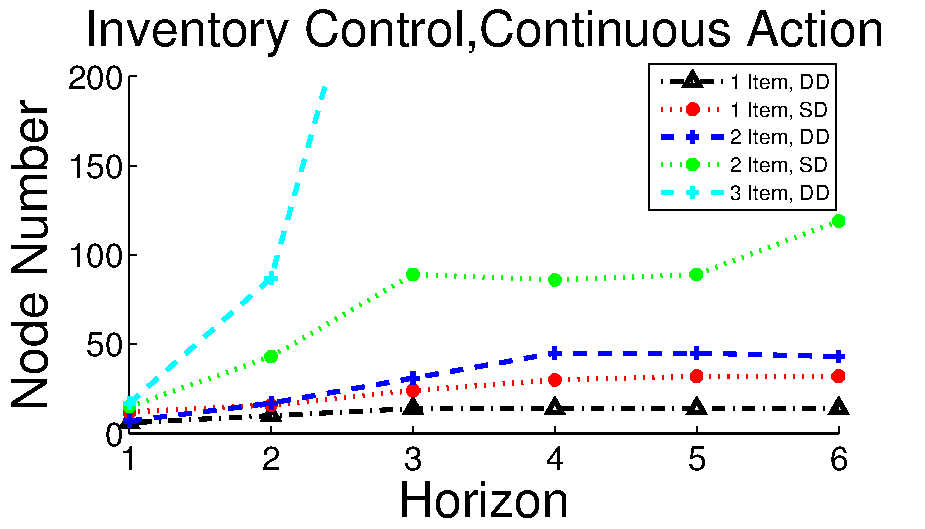
\includegraphics[width=0.45\textwidth]{pics/invCNode.pdf}
\hspace{2mm}
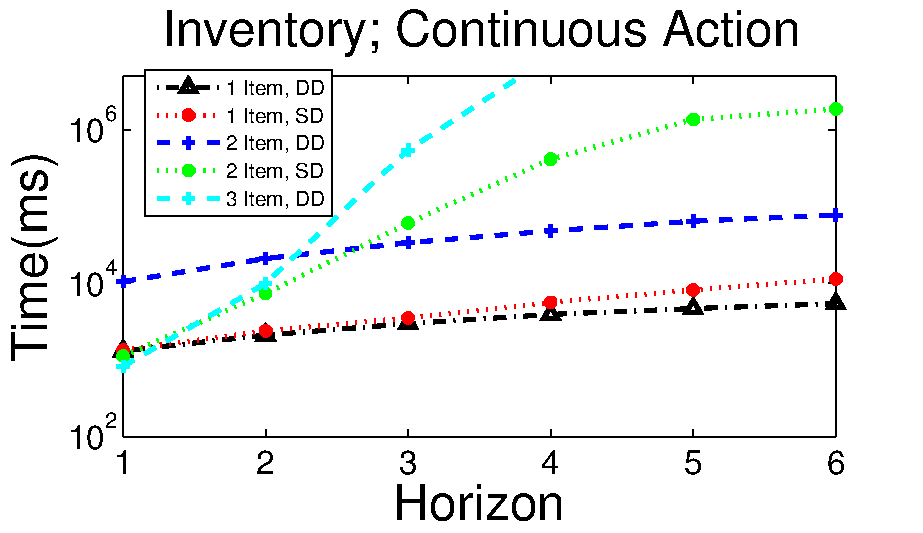
\includegraphics[width=0.45\textwidth]{pics/invCTime.pdf}
%}
\vspace{-2mm}
\caption{%\footnotesize 
\textsc{Continuous Action} \InventoryControl: space and time vs. horizon.
% comparing 
%1,2 or 3 States and actions (SA) with Deterministic (DD) 
%or Stochastic (SD) demand and no-pruning}.
}
\label{fig:invC}
\vspace{-2mm}
\end{figure}
%%%%%%%%%%%%%%%%%%%%%%%%%%%%%%%%%%%%%%%%%%%%%%%%%%%%%%%%%%%%%%%%%%%%%%%%%%
%%%%%%%%%%%%%%%%%%%%%%%%%%%%%%%%%%%%%%%%%%%%%%%%%%%%%%%%%%%%%%%%%%%%%%%%%%
%figure5 : time-iteration and space-iteraton for 1d-2d-noPrune inventory
\begin{figure}[tbp!]
\vspace{-2mm}
\centering
%\subfigure{
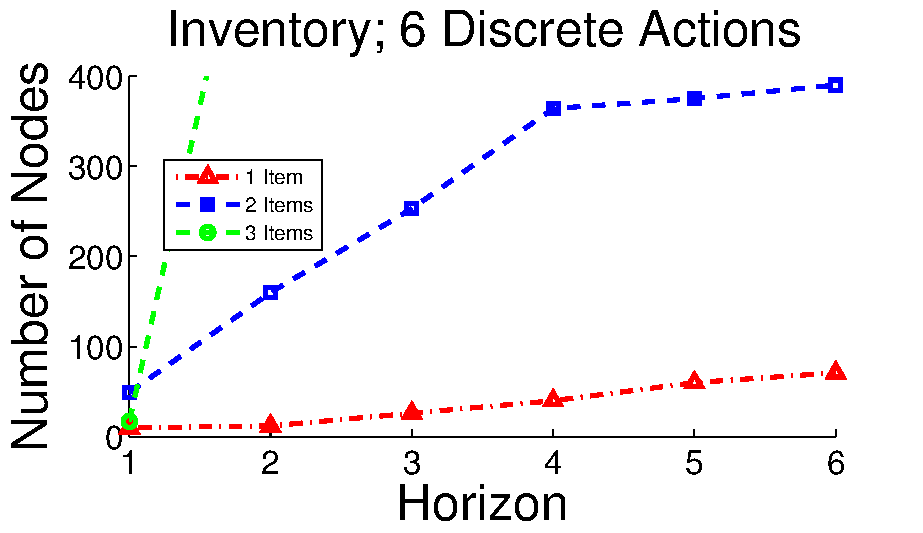
\includegraphics[width=0.45\textwidth]{pics/invD6Node.pdf}
\hspace{2mm}
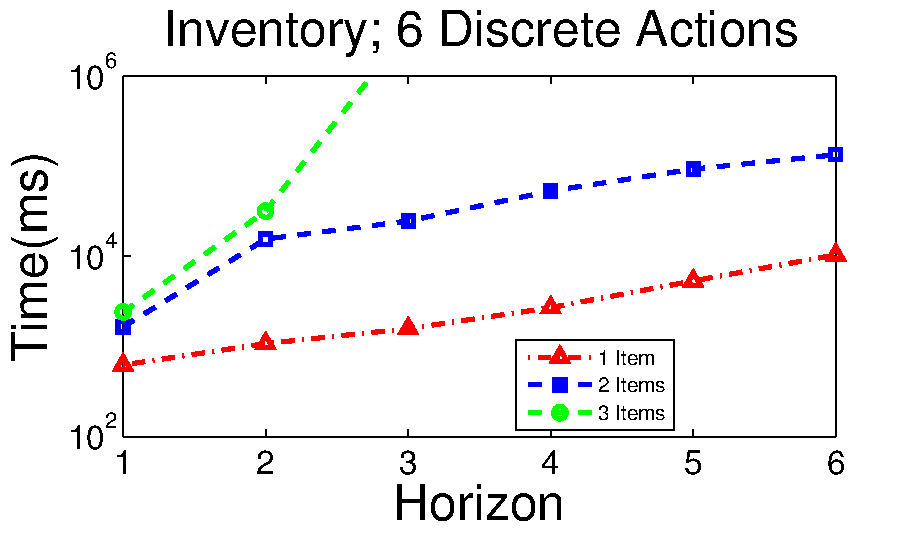
\includegraphics[width=0.45\textwidth]{pics/invD6Time.pdf}
%}
\vspace{-2mm}
\caption{%\footnotesize 
\textsc{Discrete Action} \InventoryControl: Space and time vs. horizon for 6 discrete actions. Results are shown for various continuous items in the inventory.
% comparing 
%1,2 or 3 States and actions (SA) with Deterministic (DD) 
%or Stochastic (SD) demand and no-pruning}.
}
\label{fig:invD6}
\vspace{-2mm}
\end{figure}
%%%%%%%%%%%%%%%%%%%%%%%%%%%%%%%%%%%%%%%%%%%%%%%%%%%%%%%%%%%%%%%%%%%%%%%%%%
%%%%%%%%%%%%%%%%%%%%%%%%%%%%%%%%%%%%%%%%%%%%%%%%%%%%%%%%%%%%%%%%%%%%%%%%%%
%figure5 : time-iteration and space-iteraton for 1d-2d-noPrune inventory
\begin{figure}[tbp!]
\vspace{-2mm}
\centering
%\subfigure{
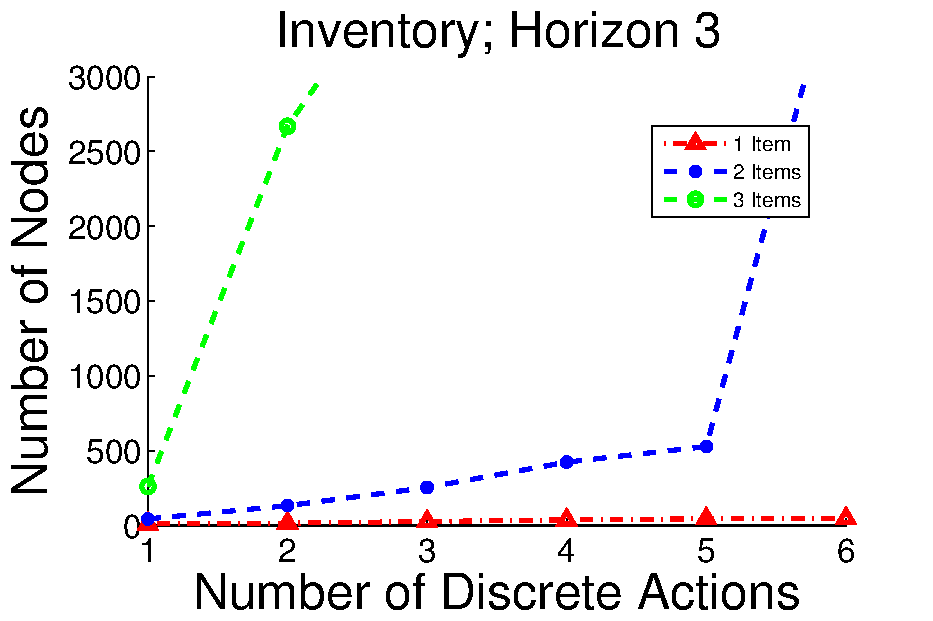
\includegraphics[width=0.45\textwidth]{pics/invH3Node.pdf}
\hspace{2mm}
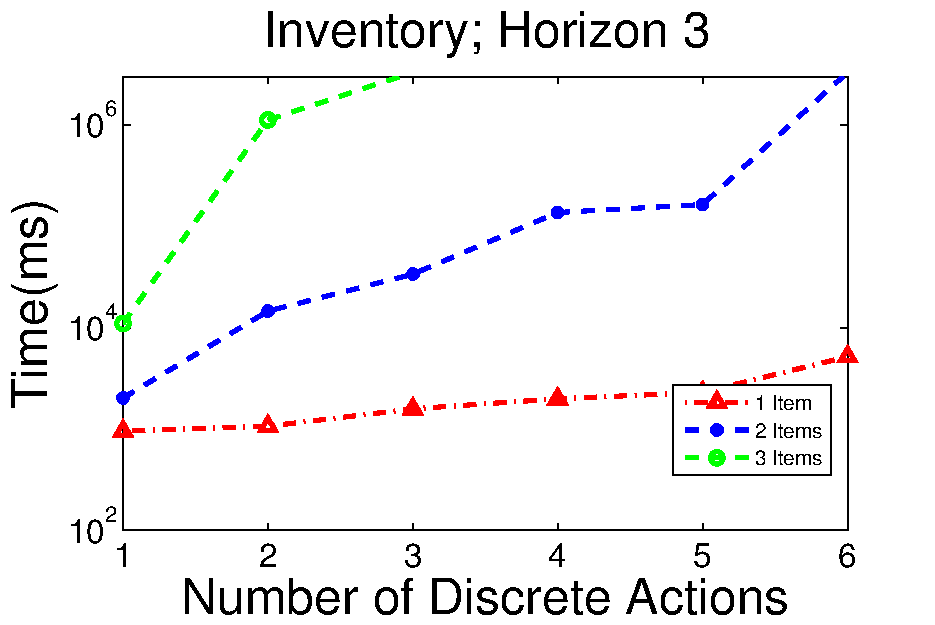
\includegraphics[width=0.45\textwidth]{pics/invH3Time.pdf}
%}
\vspace{-2mm}
\caption{%\footnotesize 
Space and elapsed time vs. horizon for a fixed horizon of 3 and different problem sizes for the \textsc{Discrete Action} \InventoryControl. 
% comparing 
%1,2 or 3 States and actions (SA) with Deterministic (DD) 
%or Stochastic (SD) demand and no-pruning}.
}
\label{fig:invH3}
\vspace{-2mm}
\end{figure}
%%%%%%%%%%%%%%%%%%%%%%%%%%%%%%%%%%%%%%%%%%%%%%%%%%%%%%%%%%%%%%%%%%%%%%%%%%

Figure~\ref{fig:invH3} illustrates the effect of different number of action discretizations for the \InventoryControl. Time and space are presented for the fixed horizon of $h=3$ and for inventory items of $1,2$ and $3$. For a 1-item inventory, as the number of discrete actions increases, the time and space grows almost linearly. However for there is an exponential blow-up of the number of nodes for the 2-item inventory beyond 5 discrete actions while the time increases dramatically. Similar to the previous experiment, the 3-item inventory problem does not scale for more than two discrete actions due to the complexity in the action space. As a result of comparing the continuous and discrete action setting for the 2-item \InventoryControl problem, the advantage of the continuous action H-MDPs is obvious. 

Finally the key point evident in the results is the fact that scaling to higher dimensions requires large amounts of memory and time. This may be achievable using faster hardware, however a more efficient solution is to scale our XADD framework.

\section{Related Work}

The most relevant vein of related work for DA-HMDPs is that of \cite{feng04} and \cite{li05} which can perform exact dynamic programming on
HMDPs with rectangular piecewise linear reward and transition functions
that are delta functions.  While SDP can solve these same problems,
it removes both the rectangularity and piecewise restrictions on the
reward and value functions, while retaining exactness.  
Heuristic search approaches with formal guarantees 
like HAO* \cite{hao09} are an attractive future extension of SDP;
in fact HAO* currently uses the method of \cite{feng04}, which could
be directly replaced with SDP.  While \cite{penberthy94} has considered
general piecewise functions with linear boundaries (and in fact,
we borrow our linear pruning approach from this paper), this work
only applied to fully deterministic settings, not HMDPs.

Other work has analyzed limited HMDPS having only one continuous
state variable.  Clearly rectangular restrictions are meaningless with
only one continuous variable, so it is not surprising that more
progress has been made in this restricted setting.  One continuous
variable can be useful for optimal solutions to time-dependent MDPs 
(TMDPs) \cite{boyan01}.  Or phase transitions can be used to 
arbitrarily approximate one-dimensional continuous distributions
leading to a bounded approximation approach for arbitrary single continuous
variable HMDPs \cite{phase07}.  
While this work cannot handle arbitrary stochastic
noise in its continuous distribution, it does exactly solve HMDPs
with multiple continuous state dimensions.

There are a number of general HMDP approximation
approaches that use approximate linear programming \cite{kveton06}
or sampling in a reinforcement learning style approach \cite{munos02}.
In general, while approximation methods are quite promising in
practice for HMDPS, the objective of this paper was to push
the boundaries of \emph{exact} solutions; however, in some sense, 
we believe that more expressive exact solutions may also inform
better approximations, e.g., by allowing the use of data structures
with non-rectangular piecewise partitions that allow higher fidelity
approximations.

%As for continuous actions and states, there has been prior work on approximate solutions to continuous state MDPs \cite{munos02,phase07} and even continuous state and action
%MDPs \cite{kveton06}, which might inform future approximate extensions
%of this work.  
As for CA-HMDPs, there has been prior work in control theory. The field of linear-quadratic Gaussian (LQG) control \cite{lqgc} which use linear dynamics with continuous actions, Gaussian noise, and quadratic
reward is most closely related.  However, these exact solutions do
not extend to discrete and continuous systems with \emph{piecewise}
dynamics or reward.
%Perhaps the most practical extension
%for future work would to combine SDP with the initial state focused
%dynamic programming techniques \cite{hao09} to increase exact solution
%efficiency when the initial state is known.
%
%While it should be theoretically possible to relax some of the 
%constraints of our setting to nonlinear dynamics or more general
%nonlinear rewards, we have carefully chosen our restrictions 
%to ensure \emph{linear piecewise boundaries}, which permit the use
%of fast linear feasibility checkers (for XADD pruning) that has proved
%critical for efficiency in problems like \InventoryControl.  Hence we
%believe this work carefully balances the tradeoff between expressivity
%and computational efficiency.  
Combining this work with initial state focused techniques \cite{hao09}
and focused approximations that exploit optimal value
structure \cite{apricodd} or further
afield \cite{munos02,kveton06,phase07} are promising directions for
future work.
% more future work for continuous actions? 


\section{Concluding Remarks}

In this paper, we introduced a new symbolic approach to solving continuous problems in HMDPs exactly. In the case of discrete actions and continuous states, using arbitrary
reward functions and expressive nonlinear transition functions far exceeds the exact solutions possible with existing HMDP
solvers.  
As for continuous states and actions, a key contribution is that of \emph{symbolic constrained
optimization} to solve the continuous action maximization problem. We
believe this is the first work to propose optimal closed-form
solutions to MDPs with \emph{multivariate} continuous state \emph{and}
actions, discrete noise, \emph{piecewise} linear dynamics, and
\emph{piecewise} linear (or restricted \emph{piecewise} quadratic)
reward; further, we believe our experimental results are the first
exact solutions to these problems to provide a closed-form optimal
policy for all (continuous) states.

While our method is not scalable for 100's of items, it still represents
the first general exact solution methods for capacitated multi-inventory control problems. 
And although a linear or quadratic reward is quite limited but it has appeared useful for single continuous resource or continuous time problems such as the water reservoir problem. 

In an effort to make SDP practical, we also introduced
the novel XADD data structure for representing arbitrary piecewise
symbolic value functions and we addressed the complications that
SDP induces for XADDs, such as the need for reordering and pruning the decision
nodes after some operations.  All of these are substantial contributions
that have contributed to a new level of expressiveness for HMDPS
that can be exactly solved.

There are a number of avenues for future research.  First off, it is
important examine what generalizations of the transition function used
in this work would still permit closed-form exact solutions.  In terms
of better scalability, one avenue would explore the use of initial
state focused heuristic search-based value iteration like
HAO* \cite{hao09} that can be readily adapted to use SDP.  Another
avenue of research would be to adapt the lazy approximation approach
of \cite{li05} to approximate HMDP value functions as piecewise
linear XADDs with linear boundaries that may allow for better
approximations than current representations that rely on rectangular
piecewise functions.  Along the same lines, ideas from
APRICODD \cite{apricodd} for bounded approximation of discrete ADD
value functions by merging leaves could be generalized to XADDs.
Altogether the advances made by this work open up a number of
potential novel research paths that we believe may help make
rapid progress in the field of decision-theoretic planning
with discrete and continuous state.

With the current solution for continuous states and actions, we can apply our methods to real-world data from the Inventory literature with more exact transitions and rewards. Fully stochastic distributions are required for these problems which is a major future direction by in-cooperating a noise parameter in the models. 
Also we have looked into value iteration for both problems, solving the symbolic policy iteration algorithm for problems with simple policies can prove to be effective in certain domains. 
The other promising direction is to extend the current exact solution for non-linear functions and solving polynomial equations using computational geometric techniques. 

\section*{Acknowledgements}

%\appendix

\vskip 0.2in
\bibliography{exactsdp}
\bibliographystyle{theapa}

\end{document}